\documentclass[12pt,oneside]{book}
\pagestyle{headings}

% Note that the line below could be modified to suit a
% particular system since the "geometry" package behaves
% differently in Unix, Windows and Mac, especially for the
% top margins.
% Adjust the parameter "top" (measuring the height of the
% space allocated to a header) and "headsep" (measuring
% the distance from the bottom of the header to the
% first line of text.
\usepackage[top=1.3in,left=1.5in,bottom=1in,right=1in,headsep=0.5in]{geometry}

\usepackage{setspace}
\onehalfspacing
%\doublespacing

% Headers and footers for thesis
\usepackage{fancyhdr}

\markboth{}{}
\newcommand\startchapter[1]{\chapter{#1}\thispagestyle{myheadings}}
\newcommand\startappendix[1]{\chapter{#1}\thispagestyle{myheadings}}
\newcommand\startfirstchapter[1]{\chapter{#1}}

% Manual addition of section to Table of Contents
\newcommand\TOCadd[1]{\newpage\phantomsection\addcontentsline{toc}{chapter}{#1}}

% Float Customization
\renewcommand{\floatpagefraction}{0.01}

% Customization of Tables of Contents and List of Figures/Tables
\usepackage{tocloft}
\renewcommand\cfttabpresnum{Table\ }
\renewcommand\cfttabnumwidth{0.75in}
\renewcommand\cftfigpresnum{Figure\ }
\renewcommand\cftfignumwidth{0.80in}
\newcommand{\HRule}{\rule{\linewidth}{0.5mm}}


% Long Table and decimal aligned columns
\usepackage{dcolumn}
\usepackage{longtable}

% Mathematics support
\usepackage{amsmath}
\usepackage{amsthm}
\usepackage{amssymb}


% Text Control
\usepackage{xspace}
\usepackage{textcase}

% Graphics
\usepackage{wasysym}
\usepackage{graphics}
\usepackage{graphicx}
\usepackage{float}
\usepackage{subcaption}

% Algorithm
\usepackage{algorithm}
\usepackage{algorithmic}
\usepackage[T1]{fontenc}

% Code
\usepackage{listings}
\usepackage{color}

\definecolor{dkgreen}{rgb}{0,0.6,0}
\definecolor{gray}{rgb}{0.5,0.5,0.5}
\definecolor{mauve}{rgb}{0.58,0,0.82}

\lstset{frame=tb,
  language=C,
  aboveskip=3mm,
  belowskip=3mm,
  showstringspaces=false,
  columns=flexible,
  basicstyle={\small\ttfamily},
  numbers=none,
  numberstyle=\tiny\color{gray},
  keywordstyle=\color{blue},
  commentstyle=\color{dkgreen},
  stringstyle=\color{mauve},
  breaklines=true,
  breakatwhitespace=true
  tabsize=3
}

\newcommand*\xor{\mathbin{\oplus}}


% Define some commands for easy typing
\newcommand{\etal}{et al. }
\newcommand{\blob}{\textit{BlobTree }}
\newcommand{\blobns}{\textit{BlobTree}}

\begin{document}

% Front Matter
\input frontmatter/fm

\newpage

%The structure of my thesis break-down into several chapters. Each chapter relates to one phase of the project
	%\newcommand{\etal}{et al. }
%\newcommand{\blob}{\textit{BlobTree }}
%\newcommand{\blobns}{\textit{BlobTree}}


\startfirstchapter{Introduction}
\label{chapter:introduction}
\section{General aim of this Research}
The goal of this thesis is to develop a framework for physically based animation of soft tissues which are increasingly used in
games, movies and simulation systems. Although at this stage this physically-based model is a goal in itself, it is hoped that
it will eventually be used for clinical predictions and for research on the influence of deformations on the functional properties 
of deformable tissues. In order to demonstrate this potential, preliminary studies in that direction are reported in the final chapter
of this thesis. To that end, a skull craniotomy simulation scenerio is created which showcases the contributions of this research in an
interactive surgical scenario. 

In this research we tackled three main problems found in the domain of soft tissue simulation and has been the topic of interest for many
researchers in the field. First, our proposed modeling solution captures the key advantages found in volumetric modeling approaches using 
implicit surfaces \cite{Bloomenthal1997, Wyvill1986, Wyvill1999, Wyvill1996, Wyvill1997, Schmidt2006, Bernhardt2010a}. Automatic blending and compact 
representation are the major benefits of using implicit surfaces for modeling. In addition, the ability to perform inside-outside tests 
easily is an inherent advantage in implicit models when implementing physically based simulations requiring collision tests. 
The \blob \cite{Wyvill1999} combined blending, affine transformations and constructive solid geometry (CSG) operators in a 
comprehensive and compact scene graph data-structure. \blob provides the ability to create complex models incrementally \cite{Schmidt2006}. 
However, volumetric models in general are often several orders of magnitude slower during visualization \cite{Bloomenthal1990a, Bloomenthal1997}.
We proposed a data-driven algorithm for rendering complex implicit models in realtime on multi-core processors \cite{Shirazian2012}, later, we 
fine tuned that algorithm for running on many core architectures such as the ones in high-end graphical processing units (GPUs). 

In traditional animation systems based on key-framing, specifying the motion and the successive shapes of objects interacting with a simulated 
world requires a great amount of specialized knowledge and intuition from the animator. Models based on simplified physical laws have been 
proposed for automating these tasks. They generate motion and deformation from initial conditions and from a set of externally applied forces 
over time, and automatically detect and respond to collisions. These models are particularly appropriate for facilitating the animation of 
deformable objects. They can either be used alone for the simulation of inanimate bodies, or be combined with user-controlled structures as 
has been done for instance in character animation \cite{chadwick1989layered,miller1988motion}. We show that a number of problems that are difficult
to solve with previous models can be easily handled by combining them with an external layer based on implicit surfaces. The implicit formulation
defines a smooth surface around the object that can be used to perform efficient collision detection, to enable exact contact modeling, and to ease
volume preservation. The second contribution of our research is the high performance volume discretization technique and non-linear finite element 
formulation to support the elastic deformations of the created models \cite{Shirazian2013}. 

In modern interactive simulation and modeling enviroments the ability to cut 3-dimensional geometry in realtime is of fundamental importance. 
This creates the need for efficient cutting algorithms that process the underlying representation. Such methods can be utilized in a wide spectrum 
of applications including surgical interventions, free form modeling, or scientific visualization. In surgery simulation, for instance, interactive 
cutting algorithms enable the dynamic simulation of scalpel intersections that open immediately behind the scalpel \cite{Nienhuys2001}. In the 
case of free-form modeling or sculpting, dynamic cutting supports a precise positioning and guidance of a cutting tool. In scientific visualization, 
real-time cutting algorithms create new opportunities for the interactive analysis of volume data sets. Seismic data sets, as an example, can be 
cut arbitrarily along interesting strata. The third main contribution of our research is our GPU-assisted interactive cutting algorithm that allows
arbitrary cuts in the model and can enable many scenarios for tissue manipulation and sensing. 

In what follows, the implicit modeling approach to deformable tissue modeling will be studied. To achieve the initial goal of this research, a
computational framework for designing, rendering and animating deformable tissues has been developed which has the potential to be used in any 
simulation system requiring deformable tissues with some level of interaction and topolgy modification. The final chapter of this thesis is dedicated
for the evaluation of our system and analysis of some example scenarios in which our system might be a good fit for. 


\section{Deformable Models}
Deformable models can be defined in either one dimension (lines and curves), two dimensions (surfaces), or three dimensions (solid objects). 
Essentially, they are applied in three different areas of research \cite{Meier2005}: 

\begin{itemize}
 \item Object modeling for pre-computed animations \cite{coquillart1990extended, hsu1992direct}.
 \item Image segmentation (automatic 2D interpretation of the images provided by a camera or 3D reconstruction of organs from medical MRI 
 or CT scans) \cite{neveu1994recovery}.
 \item Interactive medical simulations i.e. to emulate the deformational behaviour of non-rigid objects due to external influences.
\end{itemize}

Our solution is targeted for the last area where it can be used both in deferred application like surgery planning (e.g., simulation of the 
outcome of craniofacial surgery) \cite{bro1995modelling, keeve1996craniofacial} and in real-time applications. These real time applications 
include image guided surgery \cite{Szekely2000}, minimally-invasive or tele-surgery and surgery simulation. 

From the number of applications, it is obvious that there is no single deformable model that is appropriate for all of the above mentioned 
problems. Instead, there are a variety of methods that are optimized in different ways to meet specific needs. Even though virtual reality 
applications of deformable models are becoming more and more frequent, in many cases, the governing prerequisite for the simulation of 
mechanical deformations has been interactivity rather than precision. In addition to that, many of the modelled objects like garments or soft 
tissues do not possess easily describable properties. Consequently, exact methods, in general, cannot be applied as deformable models, and thus, 
other approaches must to be found \cite{bro1998finite}. Important progress in the field of deformable models has been made since the emergence of surgery 
simulation, with one of the first contributors being Cover et al. \cite{cover1993interactively}. This is mostly due to the extreme prerequisites 
as far as computation time, complex properties of the simulated soft tissues, and intricate interactions with the virtual instruments are concerned. 
In fact, there have been many different points of departure in the research of adequate deformable models, focusing on anatomies and surgical techniques 
that are as different from each other as are eye surgery \cite{cai2001parametric, sagar1994virtual}, knee arthroscopy \cite{gibson1997simulating, 
hoffman1998commercially}, or hepatic laparoscopy \cite{cotin1999real}. The deformable models developed in this context can be divided into three basic groups: 

\begin{enumerate}
 \item The ad-hoc heuristic methods
 \item Simplified continuum-mechanical model
 \item Hybrid methods from the combination of 1 and 2
\end{enumerate}

\section{Motivation}
One of the most important changes in the past decade has been the laparoscopic surgery which brought new technologies into the operating room and created a 
distance between the surgeon and the patient. More recently, other minimally invasive techniques have been proposed, such as natural orifice transluminal 
endoscopic surgery, which can be considered as an evolution of the laparoscopic surgery. As a new surgical technique, laparoscopy requires surgeons to acquire 
new skills, and adapt to changes from conventional open surgery (e.g. amplified tremor, diminished tactile sensation, loss of depth perception). This has been 
a motivation for a number of works in the field of surgery simulation, real-time deformable models, or haptic rendering \cite{Lin2004}. The following benefits are reported
from using the surgical simulation systems:

\begin{itemize}
 \item Systematic training and objective assessment of technical competence
 \item Skills learned thanks to the simulator are transferrable to the operating room
 \item The ability to create patient-specific simulations (i.e. rare pathological cases or when the best surgical strategy is unclear.)
 \item The ability to use augmented reality for image-guided surgery (i.e. to improve the accuracy and limit the adverse effects of surgery)
\end{itemize}

In order to accomplish these goals, accurate, real-time biomechanical models are needed, but their interactions with medical devices also needs to be modeled.
Such interactions not only involve tissue manipulation, but also tissue dissection. 

In this context, modeling and high-performance rendering of soft-tissues are the core requirements for any simulation scenarios. 
The development of fast algorithms to compute the deformation, contact response, cutting and haptic feedback of soft tissues could enable a number of the 
aforementioned applications.

More specifically, when considering requirements for realistic interactive simulations of medical procedures, several elements seem mandatory: anatomical 
models and tissue properties need to be patient-specific and obtained without complex additional procedure; soft tissue behaviour needs to be realistic and 
demonstrate a predictive capability, yet it should be compatible with real-time computation; interactions with the surrounding anatomy and with medical 
devices need to involve advanced contact models that can be computed in real-time; the different types of dissection performed on soft tissues should be 
simulated; and finally realistic visual and haptic feedback should be provided to create a higher level of immersion, in particular during training sessions.

\section{Limitation of Current Models}
%%Chapter \ref{chapter:background} will provide more details on the state of the art techniques in soft tissue modelling. 
Among the numerous publications in the field of biomechanics, realtime deformable models, collision detection, contact modelling or haptics, 
few methods have been proposed to address at least a majority of the requirements listed above. Among the existing approaches which at least 
partially aim at this objective, we can cite methods based on spring-mass networks, methods based on linear elasticity, and explicit finite element models 
for non-linear materials \cite{Gibson1997a,Meier2005}. In chapter \ref{chapter:background} we discuss these methods in detail.  

Mass-spring networks are quite simple to implement and very fast to compute, but they fail to properly characterize soft tissues deformation as they 
introduce artificial anisotropy through the choice of the mesh, and make it difficult to relate spring stiffness to material properties such as Young modulus 
\cite{Courtecuisse2010}.

Most methods based on the Linear elasticity made the assumption of small displacements and relied on pre-computed response in order to accelerate the 
computations. The small strain assumption is very restrictive. In addition, during any topogical modifications e.g. in cutting, the pre-computed values 
has to be recalculated which masks their effectiveness in the overall performance of the system.

Cutting deformable tissues is one of the most sought after features in a surgical simulator. In interactive system with high expectations of realism and 
performance the implementation of topogical modifications can become very complex. The proposed solutions suffer from smoothness of the cutting plane or slower
solve time due to lots of extra nodes added to the system. In chapter \ref{chapter:Cutting} we review all the related work in this topic and present our
high performance cutting algorith which is built into our physically-based simulation system.


\section{Contributions}
Contributions described in this thesis fall into four broad categories: a modeling system to create complex deformable tissues under the heading of the 
\blob; a high-performance subsystem for rendering; a non-linear finite element formulation of the deformable models created with \blob scenegraph and
a high-performance topology modification algorithm to support cutting. 

The main contributions are as the following:

\begin{itemize}
 \item A comprehensive modeling framework supporting a broad set of skeletal implicit primitives, sketched primitive objects, warping, blending, 
 affine tranformations and constructive solid geometry operators in the compact \blob structure.
 \item An algorithm for interactive polygonization of implicit surfaces on multi-core architectures with SIMD instructions.
 \item An optimized GPU-assisted algorithm for high-performance polygonization of implicit surfaces on many-core architectures.
 \item A high-performance algorithm for volume discretization of \blob models which can generate tetrahedral mesh elements with respect to a triangular 
 surface mesh for finite element formulation.
 \item A non-linear finite element formulation of deformations and a GPU-assisted algorithm for fast numerical approximations.
 \item A high-performance algorithm for cutting the tissues interactively. 
\end{itemize}


\section{Overview}
In the next chapter we start by providing background material on implicit modelling technique, the \blob scenegraph and the concept of sketch-based, incremental modelling.
We continue by reviewing the physics properties of the deformable tissues and cover some topics on continuum mechanics concepts and force models used in
our system to achieve non-linear deformations. Chapter \ref{chapter:cpuPoly} presents our rendering framework to visualize complex \blob models using multi-core 
architectures. Building on the outcomes of chapter \ref{chapter:cpuPoly}, the improved results are reviewed in chapter \ref{chapter:GPUDiscretization}. 
The discretization technique to convert a \blob model to a physical system is also given in this chapter. Chapter \ref{chapter:finiteelementmethod} is 
where we discuss our accelerated finite element implementation on the GPU side. Previous attempts in modeling deformable tissues are reviewed in this chapter and
the benefits and drawbacked of all the methods are discussed. 

Chapter \ref{chapter:Cutting} presents one of the main contributions of this thesis which is the high performance soft tissue cutting. After a brief overview of the 
related work we present our novel technique in cutting complex soft tissues interactively. Chapter \ref{chapter:evaluation} showcases a skull craniotomy simulation 
scenario and provides comments on the operation itself and the achieved results.

Chapter \ref{chapter:conclusion} provides a summary of the results in the previous chapters and reviews the limitations of the current system
and some discussions on the future work in this research topic.


















	\startchapter{Background Material}
\label{chapter:background}

\newlength{\savedunitlength}
\setlength{\unitlength}{2em}
This chapter provides a short summary of the material which is relevant to the subject of this research. Starting with the concepts underlying 
implicit and deformable tissue modelling and an outline of continuum mechanics and finite element concepts, the chapter will conclude by reviewing closely related 
deformable models presented in the literature. 

\section{Implicit Modelling}
\label{sec:implicitmodellingintro}
Implicit surfaces are two-dimensional, geometric shapes that exist in three dimensional space; they can be defined based on discrete data, 
radial basis functions, offset surfaces, algebraic surfaces, level sets or distance fields to skeletal geometric primitives \cite{Bloomenthal1997}.
Independently of its origin, an implicit surface can be defined as a level-set function $F:\mathbb{R}^3 \rightarrow \mathbb{R}$ where the surface 
and the volume can be defined as following:

\begin{equation}
S = \left\{M = (x,y,z) \in \mathbb{R}^3 | F(x,y,x) = c\right\}
\end{equation}

\begin{equation}
V = \left\{M = (x,y,z) \in \mathbb{R}^3 | F(x,y,x) \geq c\right\}
\end{equation}

$c$ is a constant and is called the \textit{iso-value} which is set to $0.5$ in our system. For each point in space if the field is greater than
$c$ the point is considered inside the model otherwise outside. 

Most of the primitives used in the \blob are built from geometric skeletons, which are incorporated in many implicit modelling software packages 
such as BlobTree.net \cite{de2008blobtree} or ShapeShop \cite{Schmidt2006}. They are ideally suited to prototype shapes of arbitrary topology 
\cite{Bloomenthal1997}. In general these works conclude that the use of skeletal primitives can lead to a simple and intuitive user modelling 
methodology. The basic building block of a skeletal primitive is a skeleton $S$. To create a skeletal primitive the distance-field $dS$ of the 
volume encapsulating the shape has to be computed as described in \cite{Barbier2004}. The distance field is a volume of scalar values which is 
not bounded as the distance itself can be infinitely large.

By modifying $dS$ with a field function $g$, it can be bound to a finite range. Usually the function maps the distances to the range $[0, 1]$, 
where the field has values of 1 at the skeletons and 0 after a certain distance to the skeleton (usually at distance 1). A discussion of field 
function appears in \cite{shirley2009graphics}. Skeletal implicit primitives are combined using binary operators, which are applied pair wise to 
field-values f, and represented by a node in the \blob, whose children are either primitives or operators themselves.
Field values are computed for the child-nodes and combined to yield a new value according to the operator type. This makes it possible to go beyond 
the classical Boolean operators, and define general blend operators that e.g. create smooth transitions between shapes. The most common operator 
that creates a smooth transition between several values is called the summation blend \cite{Bloomenthal1997}:

\begin{equation}
F_A(x, y, z)=\sum_{i=1}^{i=N_A}F_i(x, y, z)
\end{equation}

Where an implicit model $A$ is generated by summing the influences of $N_A$ skeletal elements: 
The field value due to an skeletal element at a point in 3D-space is computed as filtered distance to its skeleton 
where the filter function (i.e. falloff function) is defined as follows \cite{Wyvill1999}: 

\begin{equation}
g_\mathrm{wyvill}(x)= \left\{ \begin{array}{rl}
 1 &\mbox{ if $x\leq0$} \\
 (1-x^2)^3 &\mbox{ if $0<x<1$}\\
  0 &\mbox{ if $x\geq1$}  
  \end{array} \right.
\label{eq:WyvillFunc}
\end{equation}

In equation \ref{eq:WyvillFunc}, $x$ is clamped to the range $[0,1]$. This polynomial smoothly decreases from 1 to 0 over the valid range, with zero
tangents at each end. An important property of this skeletal primitive definition is that the scalar field is \textit{bounded}, meaning that $f=0$
outside some sphere with finite radius. Bounded fields guarantee local influence, preventing changes made to a small part of a complex model from
affecting distant portions of the surface. Local influence preserves a \textquotedblleft principle of least surprise\textquotedblright that is critical 
for interactive modelling.  

Normals can be derived from gradients which are computed by evaluating 4 field values and performing a numerical approximation:

\begin{equation}
\nabla F(x,y,z)=\left\{ \begin{array}{rl}
 F(x+\delta,y,z)-f \\
 F(x, y +\delta,z)-f \\
 F(x, y, z+\delta)-f \\
  \end{array} \right. 
\label{eq:Normal}
\end{equation}

Where $f = F(x,y,z)$ is the field at point $(x,y,z)$.
% $fv = F(x,y,z)$ be the field at a point:
%$\nabla F(x,y,z)=\frac{1}{\delta}\left( F(x+\delta,y,z)-fv \right)$

Each skeletal primitive has a bounded region of influence in space. For each node in the tree an
axis-aligned bounding box is computed which is used to trivially reject those field queries that 
are outside the box. The bounding box of the entire model is computed as the union of all primitive
nodes bounding boxes.

For evaluating the field  at a point $P$ in a \blob model such as the one shown in figure (\ref{fig:CoffeeMugBlobTree}), 
the tree structure should be traversed from root to leaves recursively. Each operator combines the values of its children 
according to its type. For example, for a simple blend the values are summed. A leaf node represents a primitive,  and 
returns the value by applying equation~\ref{eq:WyvillFunc} to the distance of $P$ from the primitive.

%The right way for inserting figures
\begin{figure}[H]
\centering
  % the following command controls the width of the embedded PS file
  % (relative to the width of the current column)
  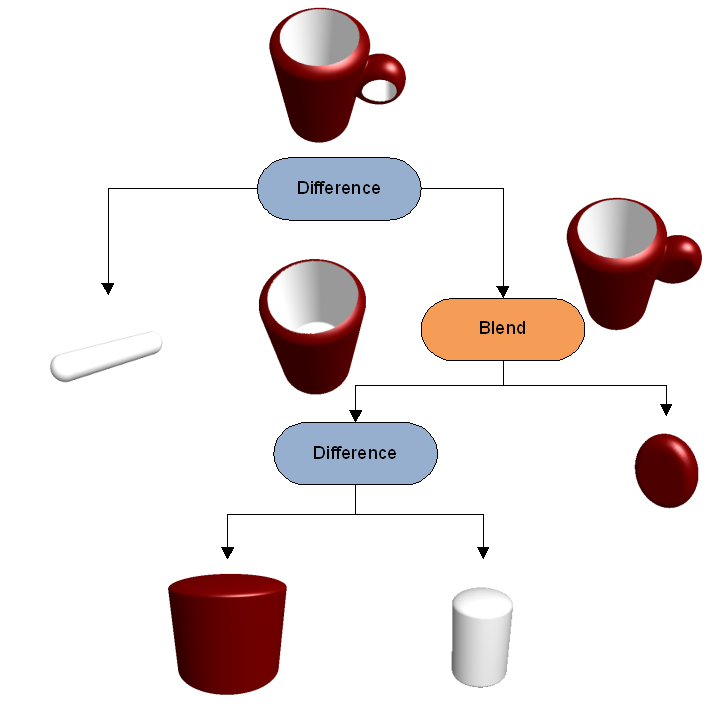
\includegraphics[width=1.0\linewidth]{figures/intro/CoffeeMugBlobTree}
  \caption{\blob structure of a coffee mug created with CSG and skeletal implicit primitives.}
  \label{fig:CoffeeMugBlobTree}
\end{figure}

%As the tree gets deeper and the number of primitives increase the computation 
For visualization purposes the \blob is queried numerous times to evaluate the field. As suggested in \cite{SWG2005} 
accelerating field computation will have a large impact on the overall surface extraction process. 

\section{Sweep Surfaces and Sketching}
Implicit primitives in our system are created from skeletons which are simple geometrical shapes such as points, line segments or 
polygons from which volumetric distance fields are created. In order to support more complex geometries \textit{Schmidt} \etal proposed the
implicit sweep objects technique where the 2D shape sketched by the user is sampled and an implicit approximation is created from 
the sample points \cite{Schmidtc}. This is done by fitting a thin-plate spline as a base shape to the sampled points using variational 
interpolation \cite{Turk1999}. One advantage of creating the base shape using variational interpolation is that the resulting implicit 
field is $C^2$ continuous, a property needed when the shape is involved in several blending operations \cite{barthe2004controllable}.

A continuous 2D scalar field is created from several field value samples $(\mathbf{m}_i, v_i)$, where $\mathbf{m}_i$ describes the 
position of the sample and $v_i$ is the desired field. The thin-plate spline used to create the variational 
implicit field $f_c(\mathbf{u})$ is defined in terms of these points weighted by corresponding coefficients $w_i$ combined with a polynomial 
$P(u) = c_1u_x +c_2u_y +c_3$.

\begin{equation}
f_c(\mathbf{u}) = \sum_{i \in N} w_i(\|\mathbf{u}-\mathbf{m}_i\|)^2ln(\|\mathbf{u}-\mathbf{m}_i\|)+P(\mathbf{u}) 
\label{eq:thinplatespline}
\end{equation}

The weights $w_i$ and coefficients $c_1$, $c_2$, and $c_3$ are found by solving a linear system defined by evaluating 
equation \ref{eq:thinplatespline} at each known solution $f_c(\mathbf{m}_i)=v_i$.
The resulting thin plate spline can then be used as the basis of several different primitives:

\begin{itemize}
 \item Inflated Objects
 \item Swept object along a trajectory
 \item Revolving object around axis
\end{itemize}

These sketched objects can then be used in the same way as the standard skeletal implicit primitives to create unique 3D shapes. Such 
unique shapes were not possible to create in previous collaborative environments, especially given the small memory footprint 
needed to transfer the information when using this technique.

\section{Deformable Models}
In their survey paper Meier \etal \cite{Meier2005} presented a classification of the deformable models available for surgery 
simulation based on their applications. The main classifications are heuristic, hybrid and continuum mechanical approaches.
Examples of heuristic models are: deformable splines, spring-mass models, linked volumes and tensor-mass models. 

With deformable splines, classical splines are employed to model a 3D object. They define a potential energy which is proportional
to the degree of elastic deformation. By using the Lagrange method, this energy is finally minimized with respect to the displacements
enforced in some control points to obtain the corresponding deformation state. The increased number of parameters required to control
the shape and the physical properties of the models will become the bottleneck and are difficult to determine empirically. A post processing
step is also required to convert the smooth spline surface to discretized polygons for rendering. Even without this post processing stage
they are computationally very expensive. E.g. solid objects have to be modelled as hollow shells which is not lending itself very well for
volume preservation applications.

\subsection{Mass-Spring Models}
Mass spring models (MSM) are the most intuitive and most common method used in deformable object modelling.
Terzopoulos \etal \cite{terzopoulos1988modelling, terzopoulos1987elastically} was the first who introduced mass-spring systems in 
computer graphics animation systems. Provot \etal showed applications of this technique in cloth simulation \cite{provot1995deformation}
as did Baraff \etal \cite{baraff1998large}. Kahel \etal used in facial animation \cite{kahler2001geometry}. 
Gibson \etal survey reviewed many examples of mass-spring system applications \cite{Gibson1997a}. In this system the deformable object
is discretized into a network of point masses which are connected with massless springs and dampers. By adding weights and considering
constant coefficient $k_s$ the elastic force is obtained by:

\begin{equation}
 \boldsymbol{f}^s_i = \sum_{j \in N(\boldsymbol{x}_i)} k_s w_{ij}(\boldsymbol{x}_{ij})(1-\frac{l^0_{ij}}{\| \boldsymbol{x}_{ij} \|})
\end{equation}

In this setup:

\begin{itemize}
 \item $\boldsymbol{x_{ij}} = \boldsymbol{x}_j - \boldsymbol{x}_i$ where $\boldsymbol{x}_i$ is the position of node $i$, 
 \item $l^0_{ij}$ is the initial spring length between node $i$ and node $j$,
 \item $N(\boldsymbol{x_i})$ is the set of neighbors of node $i$ and $w_{ij}$ is the weight of $j$th neighbor of node $i$.
\end{itemize}

The damping force in this setup is given by:

\begin{equation}
 \boldsymbol{f}^d_i = \sum_{j \in N(\boldsymbol{x}_i)} k_d w_{ij} \frac{\boldsymbol{v}^\tau_{ij} \boldsymbol{x}_{ij} }{\|\boldsymbol{x}_{ij} \|} \boldsymbol{x}_{ij}
\end{equation}
where $\boldsymbol{v}_i$ is the velocity of node $i$ and $\boldsymbol{v}_{ij} = \boldsymbol{v}_j - \boldsymbol{v}_i$.

\subsection{Linked Volumes}
\label{sec:linkedvolumes}
The ideas in MSM can be extended to volumetric modelling by discretizing the entire volume of a deformable model into evenly spaced cubic elements.
The total mass of the model is distributed at the centers of these cubes. The cubes are interconnected with their neighbors using springs and dampers
\cite{gibson1997simulating}. One of the disadvantages of this approach is its increased computational cost due to the higher number of nodes and
their increased connectivity. In order to control the computational cost for large models the resolution of the discretization should be lowered 
which will lead to unrealistic deformations. For rendering purposes auxiliary surface representations should be used such as surface maps. 
Increasing the number of elements slows down the propagation of deformations. The benefit of this approach is that complex interactions such as
cutting, carving, joining, or tearing can easily be represented by simply eliminating or adding links between elements.


\subsection{Mass Tensor Model}
Using this technique the entire interior of the model is discretized into tetrahedrons. Points masses and springs are 
being placed at the respective tetrahedral vertices and edges \cite{de1999modeling}. The performance of this model is comparable to that of the 
linked volumes describe earlier in section \ref{sec:linkedvolumes}. Cutting models created with this techniques is a challenge since even when
minimizing the number of newly created tetrahedrons in such a situation the corresponding increase of nodes in significant and directly hits the
performance of the system. The performance of the model depends on the resolution of the mesh in this case \cite{picinbono2000real}. 


\section{Continuum Mechanics Concepts} 
Continuum biomechanics for soft tissue simulation deals with the movement of soft materials when subjected to applied forces \cite{Sifakis2012}. 
The motion of a continuous and deformable solid can be described by a continuous displacement field resulting from a set of 
forces acting on the solid body. A displacement \textit{field} implies a continuous variation of displacement with position. 
The continuous displacement field can be time-independent or time-dependent. The initial unloaded state of material is referred to 
as the \textit{reference} or \textit{undeformed} state as the displacements are zero everywhere. The material then reconfigures due to 
applied loads and reaches an equilibrium state referred to as \textit{deformed} state. The concepts of \textit{strain}, a measure of length
change or displacement gradient, and \textit{stress}, the force per unit area on an infinitesimally small plane surface within the material, 
are of fundamental importance for continuum biomechanics of soft tissues. 

The formulation of models in continuum mechanics consists of three parts:

\begin{enumerate}
 \item Kinematics: Geometric description of the deformation
 \item Dynamics: A formulation of the equations of motion
 \item Constituitive formulation: Description of the material properties
\end{enumerate}

\section{Deformation map and deformation gradient}
Our initial objective is to provide a concise mathematical description of the deformation that an elastic body has sustained. This formulation will 
lay the foundation for appropriate representations of other physical properties such as force and energy. We begin by placing the undeformed elastic 
object in a coordinate system, and denote by $\Omega$ the volumetric domain occupied by the object. This domain will be referred to as the reference 
(or undeformed) configuration, and we follow the convention that capital letters $\vec{X} \in \Omega$ are used when referring to individual material
points in this undeformed shape. Note that the precise position and orientation of the undeformed elastic body within the reference space is not important 
and can be chosen at will, as long as the shape of the object corresponds to a rest configuration

When the object undergoes deformation, every material point $\vec{X}$ is being displaced to a new deformed location as seen in figure 2.1 (top) which is, 
by convention, denoted by a lowercase variable $\vec{x}$. The relation between each material point and its respective deformed location is captured by 
the deformation function $\vec{\phi} : \mathbf{R}^3 \rightarrow \mathbf{R}^3$ which maps every material point $\vec{X}$ to its respective deformed 
location $\vec{x}=\vec{\phi}(\vec{X})$.

An important physical quantity derived directly from $\vec{phi}(\vec{X})$, whose utility will become apparent in the next sections, is the deformation 
gradient tensor $\mathbf{F} \in \mathbf{R}^{3 \times 3}$. If we write $\vec{X} =(X_1,X_2,X_3)^T $ and 
$\vec{\phi}(\vec{X})=(\phi_1(\vec{X}), \phi_2(\vec{X}), \phi_3(\vec{X}))^T$ for the three components of the vector-valued function $\vec{\phi}$,
the deformation gradient is written as: 

\begin{equation}
 \mathbf{F} := \frac{\partial(\phi_1, \phi_2, \phi_3)}{\partial (X_1, X_2, X_3)}= 
 \left(\begin{array}{ccc} 
      \partial \phi_1/\partial X_1 & \phi_1/\partial X_2 & \phi_1/\partial X_3 \\
      \partial \phi_2/\partial X_1 & \phi_2/\partial X_2 & \phi_2/\partial X_3 \\
      \partial \phi_3/\partial X_1 & \phi_3/\partial X_2 & \phi_3/\partial X_3 
      \end{array} \right)
\end{equation}



or, in index notation $F_{ij} = \phi_{i,j}$. That is, F is the Jacobian matrix of the deformation map. Note that, in general, $F$ will be spatially varying 
across $\Omega$; in the next sections we will use the notation $F(\vec{X})$ if such dependence needs to be made explicit.

\section{Strain energy}
When a deformable tissue undergoes some deformation the energy will be accumulated in the object which is called \textit{strain energy}: $E[\phi]$ (We 
follow the same notation given in \cite{Sifakis2012}) The \textit{strain energy} is fully determined by the deformation map of a given configuration.
One of the characteristics of \textit{hyperelastic} materials is that their \textit{strain energy} is independent of the prior deformation history 
of the object. This property is closely related to the fact that the elastic forces of the \textit{hyperelastic} materials are \textit{conservative}.
The total work done by the internal elastic forces in a deformation path depends solely on the initial and final configurations and not the path itself.

When applying forces on a deformable tissue, different regions of the tissue will undergo shape changes of different severity. Thus, in order to compute the 
strain energy we start from a local view of the deformations. An \textit{energy density} function $\Psi[\phi; \vec{X}]$ measures the strain energy 
\textit{per unit of undeformed volume} on an infinitesimal domain $dV$ around the material point $\vec{X}$. The total energy of the deforming body is then 
computed by integrating the energy density function over the entire domain $\Omega$:

\begin{equation}
  E[\phi]=\int_\Omega\Psi[\phi;\vec{X}]d\vec{X}
\end{equation}

%todo: Add some examples for the strain energy formula

We survey a number of different simulated materials and describe how their physical properties are encoded in their respective governing equations. The 
\textit{constitutive model} is the mathematical description of the physical characteristics of a given material and includes the equations that relate
stimuli (e.g. deformations) to the material response which can be the force, stress or energy they trigger. 

\section{Strain Computation}
In principle, an explicit formula that relates $\Psi$ and $\vec{F}$ would be perfectly adequate as a constitutive equation. The challenge, with designing
constitutive models in this fashion is that using the raw elements of the matrix $F$ can be a very unintuitive way to argue about the flavor and severity
of a given deformation. It is possible that a certain material's response is dominated by its affinity for volume conservation, while a different material
might prioriatize resistance to shear. Metrics such as ``The ratio of the volumetric expansion'' or ``the shear angle'' would be much more effective in 
expressing the severity of the types of deformation that are most relevant to such materials. As a consequence, it is common for the design process for 
constitutive models to define certain intermediate quantities such as strain measures and invariants which are derived from F, yet capture the specific 
traits of the deformation that the energy or stress values depend on more concisely than the deformation gradient itself.


A strain measure is intended to be a quantitative descriptor for the severity of a given deformation, i.e. a way to gauge how far this configuration is 
from a rest configuration. For this reason, although strain measures are derived from the deformation gradient, they strive to retain as much information 
from it that is relevant to assessing deformation magnitude while disregarding any information contained in it that is unrelated to shape change. 
The deformation gradient contains all the information necessary to determine how a small neighborhood of a material point deforms. One would like, 
however, to distinguish between two important cases, namely, those in which the neighborhood of a point has just undergone a rigid motion and, on the other 
hand, those in which the neighborhood has undergone a true change of shape or of size. In the first case, the deformation gradient would correspond to a 
pure rotation. Mathematically, this phenomenon manifests itself in the fact that the matrix representing the deformation gradient $\mathbf{F}$ is a so called
\textit{orthogonal} matrix. An orthogonal matrix $\mathbf{R}$ is characterized by the property that its inverse, $\mathbf{R}^{-1}$, is equal to its transpose,
$\mathbf{R}^T$. For a pure rotation (as opposed to a reflection) the determinant of an orthogonal matrix is equal to +1 (instead of -1 for a combined rotation
and reflection). The question is: given an arbitrary $\mathbf{F}$, is it possible to separate the part that corresponds to a pure rotation from the part 
representing a true change of shape and/or of size? The answer to this question is given by a remarkable theorem in algebra known as the 
\textit{polar decomposition theorem}. It asserts that every non-singular matrix $\mathbf{F}$ can be uniquely decomposed into the product of an orthogonal 
matrix $R$ and a positive definite symmetric matrix $U$, as follows:

\begin{equation}
\mathbf{F} =  \mathbf{R}\mathbf{U}
\end{equation}

A positive definite symmetric matrix (namely, one with all positive eigenvalues) can be shown to represent pure elongations or contractions along three 
mutually perpendicular axes (the so-called \textit{principal axes}) \cite{fung2001classical}.

Consider the Green strain tensor $\mathbf{E} \in \mathbf{R}^{3\times 3}$, defined as:

\begin{equation}
\mathbf{E} = \frac{1}{2}(\mathbf{F}^T\mathbf{F}-\mathbf{I}).
\end{equation}

These axes, defined in the point at the reference configuration, are the \textit{eigenvectors} of the symmetric matrix:

\begin{equation}
\mathbf{C} =  \mathbf{F}^T\mathbf{F}
\end{equation}

known as the \textit{right Cauchy-Green tensor}. It is related to $\textbf{U}$ by the equation $\mathbf{C}=\mathbf{U}^2$.
From the preceding considerations, it follows that the neighborhood of a material point will undergo a pure rotation if, 
and only if, $\mathbf{C}=\mathbf{U}=\mathbf{I}$. Otherwise, there will be a genuine change of size and/or shape. 


It is convenient, therefore, to introduce the following measure of \textit{strain}, sometimes called the \textit{Lagrangian 
strain tensor}: 


\begin{equation}
\mathbf{E} = \frac{1}{2}(\mathbf{C} - \mathbf{I})
\end{equation}

This tensor has the property of vanishing if, and only if, there is no strain (change of shape and/or size) at the points in question.
Again there are no limitations whatsoever to the magnitude of the derivatives of the displacements used to calculate the Lagrangian
strain tensor. 


\section{Linear Elasticity}
The simplest practical constitutive model is linear elasticity, defined in terms of the strain energy density as:

\begin{equation}
\label{eq:linearelasticity}
 \Psi(\mathbf{F}) = \mu\boldsymbol{\epsilon}:\boldsymbol{\epsilon} + \frac{\lambda}{2}tr^2(\boldsymbol{\epsilon})
\end{equation}

where $\boldsymbol{\epsilon}$ is the small strain tensor and $\mu$, $\lambda$ are the \textit{Lame coefficients}, which are related to
the material properties of \textit{Young's modulus k} (a measure of stretch resistance) and \textit{Poisson's ratio} $\nu$ (a 
measure of incompressibility) as:

\begin{align*}
\mu=\frac{k}{2(1+\nu)} \hspace{10 mm} \lambda=\frac{k\nu}{(1+\nu)(1-2\nu)}
\end{align*}

The relation between the Piola stress $\mathbf{P}$ and $\mathbf{F}$ can be derived as follows:

\begin{gather*}
\delta \boldsymbol{\epsilon} =\frac{1}{2}(\delta\mathbf{F} + \delta\mathbf{F}^T)=Sym\left\{\delta\mathbf{F}\right\}  \\
\boldsymbol{\epsilon}:\delta\boldsymbol{\epsilon}=\boldsymbol{\epsilon}:Sym\left\{\delta\boldsymbol{F}\right\}=\epsilon:\delta\boldsymbol{F} \hspace{10 mm}
tr(\delta\boldsymbol{\epsilon})=\boldsymbol{I}:Sym\left\{\delta\boldsymbol{F}\right\}=\boldsymbol{I}:\delta\boldsymbol{F} \\
\delta\Psi=2\mu\boldsymbol{\epsilon}:\delta\boldsymbol{\epsilon}+\lambda tr(\boldsymbol{\epsilon})  tr(\delta\boldsymbol{\epsilon})=[2\mu\boldsymbol{\epsilon}+\lambda tr(\boldsymbol{\epsilon})]\boldsymbol{I}:\delta\boldsymbol{F}\\
Thus \hspace{10 mm} \boldsymbol{P}=2\mu\boldsymbol{\epsilon}+\lambda tr(\boldsymbol{\epsilon})\boldsymbol{I}
\end{gather*}

after one final substitution for $\boldsymbol{\epsilon}$ and a few algebraic reductions:

\begin{align*}
  \boldsymbol{P}(\boldsymbol{F})=\mu(\boldsymbol{F} + \boldsymbol{F}^T-2\boldsymbol{I})+\lambda tr(\boldsymbol{F} - \boldsymbol{I})\boldsymbol{I}
\end{align*}

These expressions allow us to make the following observations:

\begin{itemize}
 \item The stress $\boldsymbol{P}$ is a \textit{linear} function of the deformation gradient. As a result, this constitutive model is characterized by a significantly
lower computational cost that other, nonlinear materials. 

\item Since the small strain tensor was designed to be accurate exclusively in a small deformation scenario, it is more appropriate to use linear elasticity when the magnitude
of motion is small. For example, a rigid motion $\vec{\phi}(\vec{X})=\boldsymbol{R}\vec{X}+\vec{t}$ would generally produce a non-zero strain 
$\epsilon = \frac{1}{2}(\boldsymbol{R}+\boldsymbol{R}^T)-\boldsymbol{I}$ and ultimately a non-zero stress, even though no shape change has taken place. 
\end{itemize}

\section{St. Venant-Kirchhoff model}
With the understanding that the small strain tensor is a mere approximation of the rotationally invariant Green strain $\boldsymbol{E}$, it 
makes sense to attempt an improvement of the linear elasticity model by using $\boldsymbol{E}$ in the place of $\boldsymbol{\epsilon}$ is equation
 (\ref{eq:linearelasticity}):

 \begin{equation}
 \Psi(\mathbf{F}) = \mu\boldsymbol{E}:\boldsymbol{E} + \frac{\lambda}{2}tr^2(\boldsymbol{E})
 \end{equation}

This constitutive model is recognized as \textit{St. Venant-Kirchhoff} material, and is the first truely nonlinear material we will examine. The first
Piola-Kirchhoff stress tensor can be computed via a process similar to the one followed for linear elasticity:

\begin{gather*}
  \delta\boldsymbol{E}=\frac{1}{2} (\delta\boldsymbol{F}^T\boldsymbol{F}+ \boldsymbol{F}^T\delta\boldsymbol{F})=Sym\left\{\boldsymbol{F}^T\delta\boldsymbol{F}\right\}\\
  \boldsymbol{E}:\delta\boldsymbol{E}=\boldsymbol{E}:\left\{\boldsymbol{F}^T\delta\boldsymbol{F}\right\}=\left\{\boldsymbol{FE}\right\}:\delta\boldsymbol{F}
  \hspace{10 mm} tr(\delta\boldsymbol{E})=\boldsymbol{I}:\left\{\boldsymbol{F}^T\delta\boldsymbol{F} \right\}=\boldsymbol{F}:\delta\boldsymbol{F}\\
  \delta\Psi=2\mu\boldsymbol{E}:\delta\boldsymbol{E}+\lambda tr(\boldsymbol{E})tr(\delta\boldsymbol{E})=\boldsymbol{F}\left[2\mu\boldsymbol{E}+\lambda tr(\boldsymbol{E}) \boldsymbol{I} \right]:\delta\boldsymbol{F}
\end{gather*}


\begin{equation}
\label{eq:venantkirchhoff}
Thus \hspace{10 mm} \boldsymbol{P}(\boldsymbol{F})=\boldsymbol{F}\left[2\mu\boldsymbol{E}+\lambda tr(\boldsymbol{E})\boldsymbol{I}\right]. 
\end{equation}

This is a rotationally invariant model; deformations that differ by a rigid body transformation are guaranteed to have the same strain energy. As a 
consequence a St. Venant-Kirchhoff material exhibits plausible material response in many large deformation scenarios where linear elasticity would 
not be applicable. Equation (\ref{eq:venantkirchhoff}) indicates that stress is a 3rd degree polynomial function of the components of $\boldsymbol{F}$; 
after discretization, nodal forces will likewise be expressed as cubic polynomials of nodal positions.
Although the St. Venant-Kirchhoff model offers significant benefits over a linear elastic model, its scope is limited to a certain degree due to its 
poor resistance to forceful compression: as a St. Venant-Kirchhoff elastic body is compressed, starting from its undeformed configuration, it reacts 
with a restorative force which initially grows with the degree of compression. However, once a critical compression threshold is reached 
($\approx 58\%$ of undeformed dimensions, when compression occurs along a single axis) the strength of the restorative force reaches a maximum. Further
compression will be met with decreasing resistance, in fact the restorative force will vanish as the object is compressed all the way down to zero volume 
(an indication of this is that when $\boldsymbol{F} = 0$ we also have $\boldsymbol{P} = 0$). Continued compression past the point of zero volume (forcing the material to invert) will 
then create a restorative force that pushes the body towards complete inversion (reflection) along one or more axes. In practical computer simulation 
examples this behavior often manifests itself as a tendency of the material to locally tangle and invert itself when subjected to strong compressive forces 
or kinematic constraints.

 
\section{Corotated linear elasticity}
The use of the quadratic Green strain in the St. Venant-Kirchhoff guaranteed the rotational invariance of the constitutive model. At the same time, 
the increased complexity inherent in highly nonlinear materials leads to unintended side effects, such as the non-physical zero stress configurations 
of St. Venant-Kirchhoff materials under extreme compression. Corotated linear elasticity is a constitutive model that attempts to combine the simplicity 
of the stress-deformation relationship in a linear material with just enough nonlinear characteristics to secure rotational invariance.
Using the polar decomposition $\boldsymbol{F} = \boldsymbol{R}\boldsymbol{S}$ we construct a new strain measure as
$\boldsymbol{\epsilon}_c = \boldsymbol{S} − \boldsymbol{I}$, which is linear on the symmetric tensor $\boldsymbol{S}$ obtained by factoring away
the rotational component of $\boldsymbol{F}$. Replacing the small strain tensor in equation (\ref{eq:linearelasticity}) we obtain the energy for corotational 
elasticity:

\begin{equation}
\label{eq:CorotatedEnergyDensity}
  \Psi(\boldsymbol{F})=\mu\boldsymbol{\epsilon}_c:\boldsymbol{\epsilon}_c+\frac{\lambda}{2} tr^2(\boldsymbol{\epsilon}_c)=
  \mu\|\boldsymbol{S} - \boldsymbol{I} \|^2_F+(\lambda/2)tr^2(\boldsymbol{S}-\boldsymbol{I})
\end{equation}

which can be equivalently written in any of the following ways:

\begin{align}
\label{eq:CorotatedEnergyDensitySVD}
\Psi(\boldsymbol{F})=\mu\|\boldsymbol{F} - \boldsymbol{R}\|^2_F+(\lambda/2) tr^2(\boldsymbol{R}^T\boldsymbol{F}-\boldsymbol{I}) \nonumber \\
\Psi(\boldsymbol{F})=\mu\|\boldsymbol{\Sigma} - \boldsymbol{I} \|^2_F+(\lambda/2) tr^2(\boldsymbol{\Sigma} - \boldsymbol{I})
\end{align}

where $\Sigma$ is the diagonal matrix with the singular values of $\boldsymbol{F}$, from the Singular Value Decomposition 
$\boldsymbol{F} = \boldsymbol{U\Sigma V}^T$. We can show that the 1st Piola-Kirchhoff stress tensor for corotated linear elasticity is given by:
 
%(\boldsymbol{F})=
%\boldsymbol{R} \left[ 2\mu\boldsymbol{\epsilon}_c \right]
 
\begin{gather*}
\boldsymbol{P}(\boldsymbol{F})=\boldsymbol{R} \left[ 2\mu \boldsymbol{\epsilon}_c + \lambda tr(\boldsymbol{\epsilon_c}) \boldsymbol{I} \right]=
\boldsymbol{R} \left[ 2\mu (\boldsymbol{S - I}) + \lambda tr(\boldsymbol{S - I}) \boldsymbol{I} \right] \\
= 2 \mu (\boldsymbol{F-R}) + \lambda tr(\boldsymbol{R}^T\boldsymbol{F} - \boldsymbol{I})\boldsymbol{R}
\end{gather*}

The motivation behind corotational elasticity is to mimic what linear elasticity would have been, if the undeformed configuration had been rotated in the same way
as encoded in the rotational factor $\boldsymbol{R}$ from the polar decomposition. In situations where the value of $\boldsymbol{R}$ varies across the domain, 
making the transition from linear to corotated elasticity is more complex than a change of variables due to a constant rotation of the undeformed configuration. 
From a computational cost perspective, the overhead of corotated vs. linear elasticity includes the cost of the polar decomposition, and the need to employ nonlinear
solvers for certain types of simulation. 

\section{Isotropic Materials}
The two mentioned constitutive material models so far have been constructed to be rotationally invariant. This property can be formally defined using a pair of 
deformation maps $\vec{\phi_1}(\vec{X})$ and $\vec{\phi_2}(\vec{X})$, that differ only by a rigid transform, specifically:

\begin{equation}
\label{eq:rigidbodytransform}
 \vec{\phi_2}(\vec{X}) = \boldsymbol{R} \vec{\phi_1}(\vec{X}) + \vec{t}, \hspace{5mm} \text{where $\boldsymbol{R}$ is a $3\times 3$ rotation matrix}
\end{equation}

A constitutive model is rotationally invariant if and only if it guarantees that the strain energy will satisfy $E\left[ \phi_1 \right] = E\left[ \phi_2 \right]$
for any such deformation pair. An equivalant definition can be provided for the hyperelastic materials based on the strain energy density function. 
After computing the gradients we can see that any two deformations that satisfy equation (\ref{eq:rigidbodytransform}) will have deformation gradient related as
$\boldsymbol{F}_2=\boldsymbol{R}\boldsymbol{F}_1$. The energy density associated with these deformations must satisfy $\Psi(\boldsymbol{F}_1)=\Psi(\boldsymbol{F}_2)$,
leading to the following equivalant definition of rotational invariance:\\

\textbf{Definition:} A hyperelastic constitutive model is \textit{rotationally invariant} if and only if the energy density satisfies

\begin{gather*}
  \Psi(\boldsymbol{RF})=\Psi(\boldsymbol{F})
\end{gather*}

for any value of the deformation gradient $\boldsymbol{F}$ and any $3 \times 3 $ rotation matrix $\boldsymbol{R}$.
One of the consequences of this definition is that the strain energy in rotationally invariant models can be written
as a function of the symmetric factor $\boldsymbol{S}$ from the polar decomposition of $\boldsymbol{F} = \boldsymbol{RS}$, since:

\begin{gather*}
  \Psi(\boldsymbol{F}) = \Psi(\boldsymbol{RS}) = \Psi(\boldsymbol{S})
\end{gather*}

Corotated elasticity defined $Psi$ as a direct function of $\boldsymbol{S}$ (see equation \ref{eq:CorotatedEnergyDensity}). 
The need to compute polar decomposition may be avoided if we are able to express $\Psi$ as a function of some other intermediate
quantity, which is also a function of $\boldsymbol{S}$, yet also computable without an explicit polar decomposition. For instance, 
St. Venant-Kirchhoff materials defined the energy density as a function of the Green strain 
$\boldsymbol{E} = \frac{1}{2}(\boldsymbol{S}^2 - \boldsymbol{I})$, which although fully determined by $S$ can also br computed without 
an explicit polar decomposition as $\boldsymbol{E} = \frac{1}{2}(\boldsymbol{F}^T\boldsymbol{F} - \boldsymbol{I})$.

One of the distinct properties of constitutive models such as St.Venant-Kirchhoff and Corotated Linear elasticity is their \textit{isotropy}.
In simple terms, a material is isotropic if its resistance to deformation is the same along all possible orientations that such deformation 
may be applied. Rubber and metal would be examples of isotropic materials, as they do not exhibit any particular direction/orientation along
which are softer or stiffer. Steel-reinforced concrete would be an example of an anisotropic material, as its resistance to deformation is 
notably different along the direction of the steel supports, compared to a direction perpendicular to them. Human muscles are also quoted 
as an anisotropic structure, as a distinct material response is observed along the direction aligned with muscle fibers.

Isotropy is a property that is assessed on a local scale, as it is always possible to generate directional features in larger structures by 
arranging material in specific ways. In terms of quantitative criterion for isotropy, we can think of an infinitesimal \textit{spherical} 
volume of material $dV$, and consider the strain energy resulting from a prescribed deformation. Now, consider the scenario where we first 
transform the sphere $dV$ by \textit{rotating it about its center} and then apply the same deformation. In an isotropic material both
scenarios would lead to the same strain energy. This is concretely expressed using the strain energy function as follow:\\

\textbf{Definition:}A hyperelastic constitutive model is \textit{isotropic} if and only if the strain energy density satisfies

\begin{gather*}
 \Psi(\boldsymbol{FQ}) = \Psi(\boldsymbol{F})
\end{gather*}

for any value of the deformation gradient $\boldsymbol{F}$ and any $3 \times 3$ rotation matrix $\boldsymbol{Q}$. A material that is both 
rotationally invariant and isotropic would satisfy

\begin{gather*}
 \Psi(\boldsymbol{RFQ})=\Psi(\boldsymbol{F})
\end{gather*}

for arbitrary rotations $\boldsymbol{R}$ and $\boldsymbol{Q}$.\\

Using the Singular Value Decomposition $\boldsymbol{F} = \boldsymbol{U\Sigma V^T}$ we conclude that rotationlly invariant, isotropic materials satisfy:

\begin{gather*}
 \Psi(\boldsymbol{F})=\Psi(\boldsymbol{U\Sigma V^T}) = \Psi(\boldsymbol{\Sigma}).
\end{gather*}

While the strain energy for rotationally invariant materials was a function only of 6 out of 9 degrees of freedom in $\boldsymbol{F}$ (those 
captured in the symmetric $\boldsymbol{S}$), for materials that are also isotropic the energy density is actually only a function of the three 
singular values of $\boldsymbol{F}$. Equation (\ref{eq:CorotatedEnergyDensitySVD}) shows that this is certainly the case for corotated linear 
elasticity. St. Venant-Kirchhoff can also be shown to satisfy all criteria for isotropy, after some simple algebraic manipulations. An example 
of a material that is rotationally invariant but \textit{not} isotropic is described by the energy:

\begin{gather*}
 \Psi(\boldsymbol{F}) = \frac{k}{2}\vec{w}^T\boldsymbol{F}T\boldsymbol{F}\vec{w}
\end{gather*}

where $\vec{w}$ is a given constant vector. This material behaves like a zero rest-length spring along the direction $\vec{w}$, while it does
not have any resistance to deformation along directions perpendicular to $\vec{w}$.

It is possible to define an isotropic material as a function of $\Psi$ and $\boldsymbol{\Sigma}$ which encodes the only 3 relevant degrees of freedom
in $\boldsymbol{F}$, this is not necessarily the preferred approach, since the overhead of an SVD decomposition would be necessary when evaluating 
any of these quantities. St. Venant-Kirchhoff materials avoided the need for an explicit polar decomposition, by using the Green strain $E$
to convey (qualitatively) the same information as $S$, while using a computationally inexpensive formula. For isotropic materials, the purpose is served 
by the three isotropic invariants of the deformation gradient, which are equally expressive as the singular values, but can be computed inexpensively. 
Invariants are denoted by $I1$, $I2$, $I3$ (or $I_1(\boldsymbol{F})$, etc., to emphasize the dependence on $\boldsymbol{F}$) and defined as:

\begin{gather*}
I_1(\boldsymbol{F})=tr(\boldsymbol{F}^T\boldsymbol{F}), \hspace{10mm}I_2(\boldsymbol{F})=tr\left[(\boldsymbol{F}^T\boldsymbol{F})^2\right], 
\hspace{10mm}I_3(\boldsymbol{F})=det(\boldsymbol{F}^T\boldsymbol{F})=(det\boldsymbol{F})^2
\end{gather*}

Their relation to $\Sigma$ is revealed by replacing $\boldsymbol{F}$ with its SVD in the previous expressions after cancellation we obtain:

\begin{gather*}
I_1 = tr(\boldsymbol{\Sigma}^2)=\sum_{i=1}^3\sigma_i^2, \hspace{10mm}I_2=tr(\boldsymbol{\Sigma}^4)=\sum_{i=1}^3\sigma_i^4, 
\hspace{10mm}I_3=det(\Sigma^2)=\prod_{i=1}^3\sigma_i^2
\end{gather*}

After computing the derivatives of the invariants with respect to the $F$:
\begin{gather*}
 \delta I_1= \delta\left[tr(\boldsymbol{F}^T\boldsymbol{F})\right]=2tr(\boldsymbol{F}^T\delta\boldsymbol{F})=(2\boldsymbol{F}):\delta\boldsymbol{F}\Rightarrow
 \frac{\partial I_1}{\partial\boldsymbol{F}}=2\boldsymbol{F}\\
 \delta I_2 = \delta \left[ tr(\boldsymbol{F}^T\boldsymbol{F}\boldsymbol{F}^T\boldsymbol{F}\right)]=4tr(\boldsymbol{F}^F\boldsymbol{F}\boldsymbol{F}^T\delta\boldsymbol{F})=
 (4\boldsymbol{F}\boldsymbol{F}^T\boldsymbol{F}):\delta\boldsymbol{F} \Rightarrow \frac{\partial I_2}{\partial \boldsymbol{F}}=4\boldsymbol{F}\boldsymbol{F}^T\boldsymbol{F} \\
 \delta I_3=\delta \left[(det \boldsymbol{F})^2\right] = 2det\boldsymbol{F}.\delta\left[det \boldsymbol{F} \right] = 2(det \boldsymbol{F})^2\boldsymbol{F}^{-T}:\delta\boldsymbol{F} \Rightarrow
 \frac{\partial I_3}{\partial \boldsymbol{F}}=2I_3\boldsymbol{F}^{-T}
\end{gather*}

With these derivatives at hand, the strain energy density is provided as a function $\Psi(I_1, I_2, I_3)$. Using the chain rule we can compute the stress as:

\begin{align}
 \boldsymbol{P}=\frac{\partial \Psi(I_1, I_2, I_3)}{\partial\boldsymbol{F}}=
 \frac{\partial \Psi}{\partial I_1}\frac{\partial I_1}{\partial \boldsymbol{F}}+
 \frac{\partial \Psi}{\partial I_2}\frac{\partial I_2}{\partial \boldsymbol{F}}+
 \frac{\partial \Psi}{\partial I_3}\frac{\partial I_3}{\partial \boldsymbol{F}},
 \hspace{10mm}\text{or, after substitution:}\nonumber
\end{align}

\begin{equation}
\label{eq:stresspBasedOnInvariants}
 \boldsymbol{P}(\boldsymbol{F})=\frac{\partial \Psi}{\partial I_1}.2\boldsymbol{F} + 
 \frac{\partial \Psi}{\partial I_2}.4\boldsymbol{F}\boldsymbol{F}^T\boldsymbol{F} +
 \frac{\partial \Psi}{\partial I_3}.2 I_3\boldsymbol{F}^{-T}
\end{equation}

We note the additional invariant $J=det \boldsymbol{F}=\sqrt{I_3}$ that is often used in replacement of $I_3$ while defining certain constitutive models.
This quantity has an important physical interpretation as it represents the \textit{fraction of volume change} due to deformation:
a value of $J=1$ implies that volume is preserved exactly while, while $J=2$ would indicate an expansion to twice the undeformed volume and $J=0.2$
would be a compression down to $20\%$ of the rest volume.

\section{Neohookean elasticity}
One isotropic constitutive model which is defined via isotropic invariants is \textit{Neohookean elasticity}:
\begin{align}
\label{eq:NeohookeanStrainEnergy}
 \Psi(I_1, J) = \frac{\mu}{2}(I_1-3)-\mu \log(J)+ \frac{\lambda}{2} \log^2(J), \text{or equivalently}\nonumber\\
 \Psi(I_1, I_3)=\frac{\mu}{2}(I_1-\log(I_3)-3)+\frac{\lambda}{8}\log^2(I_3)
\end{align}

From this definition the following derivatives can be computed easily:

\begin{gather*}
 \frac{\partial \Psi}{\partial I_1}=\frac{\mu}{2}\hspace{10mm}\text{and}\hspace{10mm}\frac{\partial \Psi}{\partial I_3}=-\frac{\mu}{2I_3}+\frac{\lambda \log(I_3)}{4 I_3}
\end{gather*}

By substituting into equation (\ref{eq:stresspBasedOnInvariants}) we get:
\begin{align}
\label{eq:NeohookeanStress}
 P(\boldsymbol{F})=\mu\boldsymbol{F}-\mu\boldsymbol{F}^{-T}+\frac{\lambda \log (I_3) }{2}\boldsymbol{F}^{-T}\hspace{10mm}\text{by some factorization}\nonumber\\
 P(\boldsymbol{F})=\mu(\boldsymbol{F}-\boldsymbol{F}^{-T})+\lambda\log(J)\boldsymbol{F}^{-T}
\end{align}

The Neohookean model has the following properties:

\begin{enumerate}
 \item The material exhibits a very strong reaction to extreme compression. The logarithmic term in the energy: $\log^2(J)$ will approach 
 to $\infty$ as $J \rightarrow 0$ hence we will have $\Psi \rightarrow \infty$. This constructs a powerful energy barrier that strongly
 resists extreme compression. This is the only constitutive model we have seen so far that has this property, other models we discussed here
 will allow the material to compress to zero volume or even invert. While only absorbing a finite amount of energy.
 
 \item In order to make incompressible materials the second Lam\'e coefficients ($\lambda$) should be set to very large value. By setting 
 $\boldsymbol{J}=1$ in the energy term of the Neohookean elasticity, a volume-preserving formulation will be produced. Incidentally, setting a
 high value for $\lambda$ in the earlier constitutive models does not quite have the desired effect, as their respective terms scaled by $\lambda$
 do not correspond to true volume change. Setting a high value for linear elasticity would enforce:
\begin{gather*}
  tr(\boldsymbol{F}-\boldsymbol{I})=0 \Rightarrow div\left[\vec{\phi}(\vec{X})-\vec{X}\right] = 0
\end{gather*}

this will ensure that displacement field $\vec{x}(\vec{X})-\vec{X}$ is divergence free. This condition approximates volume preservation only
for small deformations.

\item If the simulated model is accidentally forced into an inverted configuration, there is no mechanism for handling that situation.  
In such cases, energy and stress are undefined, since $J <0$ (See equations \ref{eq:NeohookeanStrainEnergy} and \ref{eq:NeohookeanStress}).
Such inversions can easily occur in practice, as a result of nonphysical kinematic constraints, instability of time integration techniques,
or inadequate convergence of numerical solvers. In these situations the deformation gradient $F$ can be temporarily replaced by the nearest
physically plausible value $\boldsymbol{F'}$ with $det\boldsymbol{F'} > \epsilon$
\end{enumerate}

In designing a finite element solution there are many aspects that must be considered such as the type of formulation used e.g.
Total or updated Lagrangian, time integration scheme e.g. explicit or implicit and the type of elements used for discretization:
e.g. hexahedral (uniform cubic voxel grid or non-uniform octree based grid) or n-simplices such as tetrahedral elements. 
These design choices will impact the performance and the range of applications that can benefit from this formulation.

\setlength{\unitlength}{\savedunitlength}

	\startchapter{High Performance Rendering on Multi-Core Architectures}
\label{chapter:cpuPoly}
One of the main challenges in animating deformable tissues is their rendering which requires to support high frame-rates \cite{Shirazian2012}. 
In order to leverage the benefits offered by \blob modelling the rendering issue has to be tackled accordingly. In this chapter
we present a parallel method for speeding up the generation of a polygon mesh from an implicit model \cite{Shirazian2012}. Although the method is applicable 
to many types of implicit surfaces, we focus on surfaces generated from fields surrounding geometric  primitives,  known as skeletal implicit 
surfaces,  \cite{Bloomenthal1997} that are discussed in chapter \ref{chapter:background}. The model data structure is a tree whose leaf nodes 
are primitives, and internal nodes are operators;  the \blobns, ~\cite{Wyvill1999}.
Currently the \blob supports operations such as;  arbitrary blends, boolean operations, warping at a local and global level including contact deformations. 
Geometric transformation matrices are also stored as nodes in the tree so the data structure is also a scene graph. 

A \blob  is typically visualized by  polygonization to produce a triangle mesh to be
rasterized by the graphics processor.  Direct ray tracing  \cite{Bloomenthal1997} can also be used,
to produce high quality images.  Both methods require computation of the field value which can 
only be evaluated by traversing the \blob structure. The field due to each operator depends 
on its child nodes and the leaves are the primitives which can be any implicitly defined function; 
e.g. distance field due to geometric skeletal elements.

Implicit  modelling using the \blob has several advantages  over other modelling methods.  Various different blends are simple to represent, 
as are free-form volume deformations and constructive solid geometry operations  (CSG) \cite{gomes2009implicit}. Other operators 
 such as detecting contact, and warping surfaces accordingly (see  \cite{Grascuel1997}),  can easily be represented as nodes in the \blobns. 

 An incremental, sketch based \blob system was built by Schmidt \etal \cite{Schmidt2006}, promoting flexibility and modular design for the creation of complex models, 
and most of the earlier problems with the methodology have been overcome \cite{Bernhardt2010}. Although direct manipulation 
is possible  \cite{Schmidt2006},  very complex models can only be visualized interactively as coarse meshes. 
Hence the need for a faster polygonizer. The \blob facilitates incremental modelling, a strategy that promotes flexibility and modular design 
for creating  complex models. 

The main contribution presented here is a high performance polygonization algorithm that scales well with the 
number of physical cores and SIMD vector width available on modern processors.

As opposed to previous work that attempted to render implicit surfaces defined by static algebraic surfaces or 
volumetric scanned data, our method is data-driven where the definition of the surface can change over time. This feature 
is particularly useful in collision detection applications such as surgical simulations where the interaction
of the surgical tools and deformable tissues should be visualized in real-time \cite{Laycock2007}. 
 
In addition we have improved the performance of the algorithm that finds the intersection of a cube edge and the surface, by making use of the SIMD architecture, 
to find the intersection in a single run of a field evaluation kernel.


%We have tested our algorithm on two different processors with various number of cores and cache memory. 
The chapter is organized as follows;  In section \ref{sec:algorithm} our algorithm is explained along with 
the improvements made to the distance-field computation process. Our performance results and future 
work are presented in sections \ref{sec:results} and \ref{sec:futurework}, respectively.

%-------------------------------------------------------------------------
\section{Architecture Constraints}\label{sec:architecture}
%Jean-Luc please check
In this section we define some processor architecture constraints, i.e. minimum 
requirements from the hardware side to implement our algorithm as efficiently as possible.
The algorithm scales with the number of physical cores and the SIMD vector width available on the processor.  
See results section (\ref{sec:results}). 

Our current implementation leverages both Intel SSE with 4 float wide and Intel AVX with 8 float wide SIMD instruction sets.
Using a cache-aware technique our algorithm is designed to minimize the movement of cache lines in and out of the processor's on-chip 
memory. To this end the technique requires at least 256 kilobytes of last level cache memory per each processor core. 
The input data structures take about 192 kilobytes of memory in our implementation.

Although our test environment was Intel based, our algorithm should be implementable on any
multicore machine with SIMD instructions and sufficient cache.

\section{Naming Conventions}\label{sec:naming}
The polygonization method used, is a space partitioning algorithm based on \cite{Wyvill1986}, which uses a  uniform grid of a user 
defined cell size (\textit{cellsize}). In order to leverage the SIMD parallel computation capabilities of the processor, the bounding 
box of the model is divided into axis-aligned grids of 8x8x8 vertices where each grid is called  model partitioning unit (\textit{MPU}). 

An \textit{MPU} is $7*cellsize$ as shown in figure \ref{fig:MPU}. Each \textit{MPU} contains 7*7*7 or 343 cubic cells. An \textit{MPU}  is called \textit{empty} 
if it does not intersect with the iso-surface of the model. 
The list of all \textit{MPU}s is called the \textit{MPUSET} and a half open interval 
$[a, b)$ over \textit{MPUSET} is called an \textit{MPURANGE} which contains consecutive \textit{MPU}s from $a$ to $b-1$.
 
\begin{figure}[H]
  \centering
  % the following command controls the width of the embedded PS file
  % (relative to the width of the current column)
  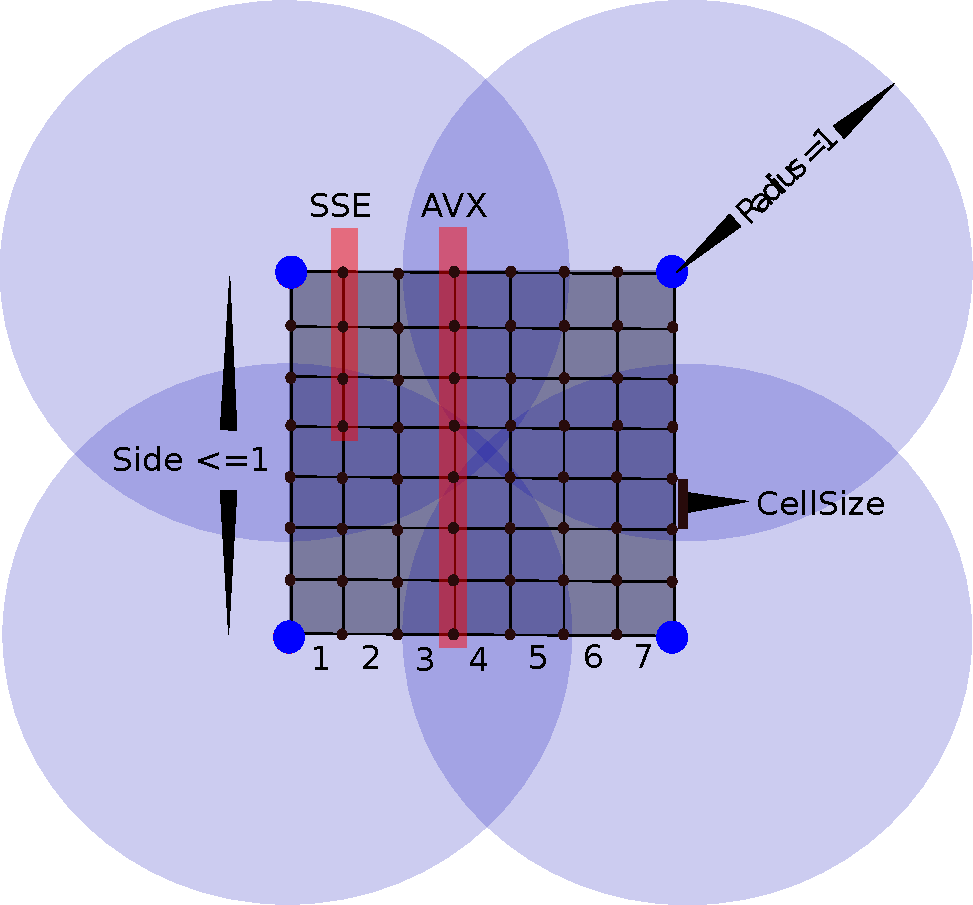
\includegraphics[width=0.7\linewidth]{figures/cpupoly/MPU.pdf}
  \caption{\label{fig:MPU}
  {The \textit{MPU} is our unit of computation per each core illustrated as a 2D cross section here. 
  Field-values due to every 4 or 8 points are computed in parallel with SSE or AVX instructions, respectively. 
  When the field at a vertex is zero no iso-surface will pass in the neighborhood of a unit circle (sphere in 3D) centered at that vertex.}
}
\end{figure}


\section{Algorithm}\label{sec:algorithm}
The input to our algorithm is a \blob data structure, representing an implicit model whose iso-surface we wish to find. Output is a 
triangle mesh.  The model bounding box and the cellsize parameter supplied by the user to control the resolution of the final mesh.
The \blob structure is first converted into a compact, linear structure required for SIMD optimization techniques, then the model 
bounding box is divided into the \textit{MPUSET} with respect to the \textit{cellsize} parameter.
The \textit{MPUSET} is processed in parallel using multiple cores; with a fast empty \textit{MPU} rejection method and SIMD surface 
extraction algorithm the mesh contained within intersecting $MPU$s is extracted. The algorithm has no synchronization points except after 
all \textit{MPU}s are processed and the triangle mesh is sent to the GPU for rasterization. The left column in figure 
(\ref{fig:AlgorithmHighLevelView}) displays these preparation steps in order.
The following sections describe this whole process in detail.


We start by describing the initialization phase and continue with the surface extraction details in the next section.
The algorithm starts by computing the size of an \textit{MPU} side (7 cells) and dividing the bounding box of the model into a 
3D grid of \textit{MPU}s, where each \textit{MPU} is assigned a unique global identifier. The main idea of our algorithm is parallel 
processing of the set of all \textit{MPU}s (\textit{MPUSET}) using multicore and SIMD processing techniques.

Our algorithm recursively splits \textit{MPUSET} into disjoint \textit{MPURANGE}s where each \textit{MPURANGE} is assigned to an idle core on 
the processor. The granularity of the divisions can be determined by the average amount of machine cycles spent to process an \textit{MPU}, 
however, in our implementation we resort to the solution provided by Intel Threading Building Blocks (TBB) \cite{Reinders2007}, 
which provides a non-preemptive task scheduling system to take care of the differences in task loads by 
monitoring processors and starting new tasks on idle cores automatically (work-stealing) \cite{Reinders2007}.


\begin{figure}[H]
  \centering
  % the following command controls the width of the embedded PS file
  % (relative to the width of the current column)
  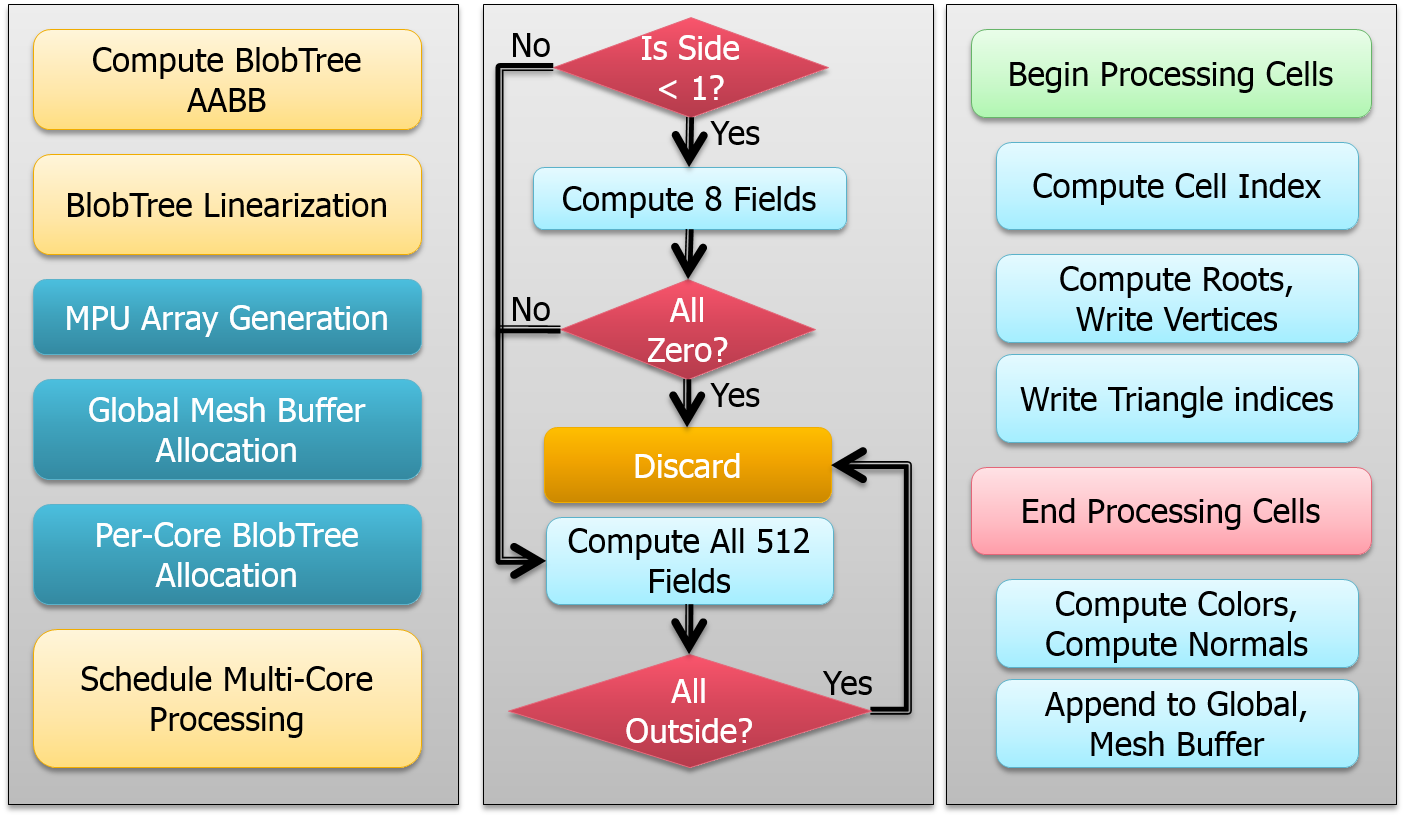
\includegraphics[width=0.9\linewidth]{figures/cpupoly/AlgorithmHighLevelView}
  \caption{\label{fig:AlgorithmHighLevelView}
  {Left Column: The one-time preparation steps before scheduling kernel functions for computation.
  Middle Column: The early discard kernel function. Right Column: The $MPU$ processing kernel function.}
}
\end{figure}

\subsection{BlobTree Linearization}\label{sec:linearization}
The first step in our algorithm is the \blob reduction and pruning as suggested by Fox \etal \cite{Fox2002}.
In the second step, using the same linearization algorithm proposed for quadtrees \cite{Lee2000}; the \blob is converted into 
a pointerless representation to achieve cache-memory efficiency by keeping all input data structures at 
aligned memory addresses and fitting the entire \blob model into the last level cache memory of the processor. 
The final linearized \blob is in the format cache-line aligned structure of arrays. With this format several computations
can be optimized with SIMD instructions, e.g. applying a transformation matrix on a vector of 4 or 8 vertices as opposed to
scalar computation. The output mesh is also in the format of cache-line aligned structure of arrays which is the key to
compute colors and normals in SIMD fashion. 



\subsection{Surface Extraction}\label{sec:surfaceextraction}
In our algorithm we assign field values for every vertex of every \textit{MPU} that is not trivially rejected with the method explained in 
the following, and compute the triangular mesh representing the iso-surface. This approach combines elements of several algorithms 
(\cite{Wyvill1986, Lorensen1987, Bloomenthal1994a}).

We extended the method proposed by Zhang \etal \cite{Zhang2006} to trivially reject all empty \textit{MPU}s.
The observation made is that according to equation \ref{eq:WyvillFunc}, if the field value at a given vertex is zero then 
the shortest distance from that vertex to the iso-surface is greater than or equal to one (See figure \ref{fig:MPU}). Using 
this fact empty \textit{MPU}s can be identified very fast by evaluating the fields at the 8 vertices of each \textit{MPU} and rejecting it of all 8 
fields are zero. However, this test is only applicable when the cellsize parameter is smaller than or equal to $1/7$ or 0.1428. 
For larger \textit{cellsize}s the iso-surface may still intersect with the \textit{MPU} while the fields at vertices of the \textit{MPU} are zero. 
This process is depicted in the middle column of figure (\ref{fig:AlgorithmHighLevelView}).
For a discussion on \textit{cellsize} versus performance see section~\ref{sec:results}.

For larger \textit{cellsize}s we shoot 8 rays from the center of the \textit{MPU} to its eight vertices, using  the technique of Zhang \etal per 
each step we march $0.866c$ (0.866 is half of the diagonal of an \textit{MPU} with side one and $c$ being the cellsize parameter) along each ray. 
At each step we compute the fields for the 8 vertices along the rays; if a non-zero field is found then the \textit{MPU} is further processed, 
otherwise we march along the rays until we reach the vertices of the \textit{MPU}. 

If an \textit{MPU} is not rejected then it is further processed for surface extraction. A local copy of the linearized \blob is provided 
per each core in order to avoid \textit{false-sharing} among cores \cite{Bolosky1993}. Using SIMD processing techniques field values for all
512 vertices of \textit{MPU} are computed. With SSE or AVX instructions this step requires 128 or 64 field evaluation kernel runs, 
respectively (figure \ref{fig:MPU}).

All the fields are stored in a memory aligned array of 512 floating points. This technique avoids reevaluating field values while processing
cells in the next step. Storing field values from a SIMD register into memory aligned address can be accomplished with a SIMD instruction in
parallel. After this step all 343 cells of the \textit{MPU} are processed. Per each cell, the 8 vertex field values 
are gathered in SIMD fashion. Each vertex with a field greater than or equal to \textit{iso-value} is labeled one otherwise zero. 
The configuration index of the cell is computed using the SIMD method shown in algorithm \ref{alg:cellconfig}. A configuration index 
is computed to access the table as in \cite{Lorensen1987}. We used the modified marching cubes table proposed by Dietrich \etal that eliminates many 
of the degenerate triangles produced in the original MC algorithm \cite{Dietrich2009}. For the ambiguous cases we take another sample 
from the center of the cell \cite{Wyvill1986, Dietrich2009}. 

%bw - make this English
\begin{algorithm}[H]
\caption{SIMD computation of cell configuration. Pseudo code provided for AVX SIMD computation. Similar code can be written in SSE.}
\label{alg:cellconfig}
\begin{algorithmic}[1]	
  \STATE Gather the 8 vertex field values of the cell  
  \STATE simd $index = cmp\_ge8(fields, simd(0.5))$
  \STATE $index = and8(index, simd(1.0))$
  \STATE $index = mul8(index, maskPower)$  
  \STATE $index = hadd8(index, index)$   
\end{algorithmic}
\end{algorithm}

In algorithm (\ref{alg:cellconfig}) fields is an array of 8 vertex field values, 
line 2 performs a parallel comparison between \textit{iso-value} and fields. 
In line 4 maskpower shifts the field values into the appropriate slot in the SIMD array and finally line 5
performs a horizontal add operation on the values to compute the configuration index.

For each intersecting edge there is one inside and one outside vertex.
Using a root finding method the point of intersection of the iso-surface is computed and stored in a 
hash table to be reused by the neighboring cells that share that vertex. 

For the root finding methods that do not require gradient information such as regula falsi or bisection method, 
the field value should be evaluated multiple times along the edge, which will degrade the performance of the system. Other methods 
such as Newthon-Raphson require gradient information, and as mentioned in equation (\ref{eq:Normal})
each gradient computation involves 4 extra field evaluations. We describe a root finding
%%%  is this really new???/ 
technique based on SIMD instructions that computes the root with only one extra field evaluation in AVX (two with SSE) 
with adequate precision. By subdividing the intersecting edge into 8 vertices and evaluating the field values, the exact interval 
containing the final root can be identified. Performing linear interpolation in that interval will produce the 
final root (figure \ref{fig:root}), it is trivial to show when the number of intervals increases the interpolation error decreases \cite{Matthews1987}. 

\begin{figure}[H]
  \centering
  % the following command controls the width of the embedded PS file
  % (relative to the width of the current column)
  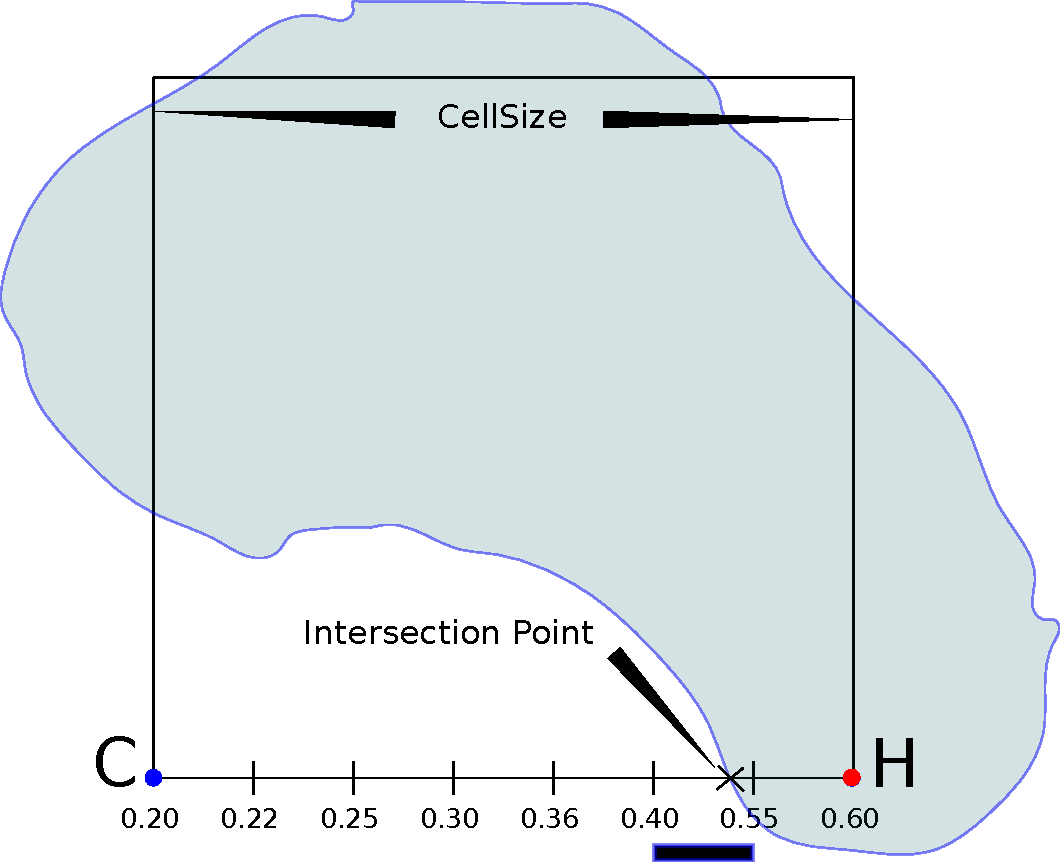
\includegraphics[width=0.8\linewidth]{figures/cpupoly/root.pdf}
  \caption{\label{fig:root}
  {Top: A cell edge is intersected with part of the surface shown in blue.  By performing one field evaluation using 
  AVX or two with SSE instructions the interval containing the intersection point can be identified. 
  The final root is computed using linear interpolation within the interval marked with bold line segment.}
}
\end{figure}


Algorithm (\ref{alg:surfaceextraction}) summarizes the process of surface extraction which is run per each \textit{MPU}. 
Lines 1 through 25 are related to the \textit{MPU} discard method explained earlier in this section. Lines 26 through 42
shows the cell processing technique which is optimized using SIMD cell configuration computation and our root 
finding method. Since color and normal attributes should only be computed for final mesh vertices, this step is 
performed last to fully leverage SIMD optimizations by performing every 4 or 8 attribute computations in 
one SIMD call which greatly enhances the throughput of the system and minimizes \blob traversals.

%%bw check this for undefined stuff - make ENglish
\begin{algorithm}
\caption{Algorithm for surface extraction of an \textit{MPU} using AVX SIMD instructions,
Similar code can be written for SSE instruction set. 
Input is linearized \blob $T$, lower vertex of \textit{MPU} and the \textit{cellsize} parameter. 
Output is the local mesh contained in the \textit{MPU}}
\label{alg:surfaceextraction}
\begin{algorithmic}[1]		
	\STATE $side \gets cellsize*7$
	\STATE simd $v \gets $Compute \textit{MPU} vertices
	\IF{$side \leq 1$}	
	\STATE simd $f \gets T.compute\_field8(v)$
	  \IF{$f == 0$}
	  \STATE return;
	  \ENDIF	
	\ELSE 
	  \STATE $flag \gets true$
	  \STATE $incr = 0.866*cellsize$	  
	  \STATE $d = incr$
	  \WHILE{$d \leq side * 0.866$}	
	  \STATE Shoot rays from center of \textit{MPU} to its 8 vertices
	  \STATE simd $v \gets $Travel along the rays for distance $d$     
	  \STATE simd $f \gets T.compute\_field8(v)$
	  \IF{$f != 0$}
	  \STATE $flag \gets false$
	  \STATE $break$;
	  \ENDIF
	  \STATE d = d + incr;
	  \ENDWHILE	
	  \IF{$flag == true$}
	  \STATE return;
	  \ENDIF	
	\ENDIF	
	
	\STATE float fieldCache[512];
	\FORALL{simd $vertex$ in $mpu$ vertices}
	\STATE simd $f \gets T.compute\_field8(vertex)$
	\STATE Store $f$ in appropriate location in $fieldCache$
	\ENDFOR
	
	
	\FORALL{$cell$ in $mpu$}
		\STATE $f \gets gather8(cell, fieldCache)$
		\STATE $edges \gets $Compute cell config from $f$ to access table
		\FOR{$i=1 \to $count of edges}
			\IF{root for $i$th edge is not stored in edge table}
			\STATE Compute and store root associated with $i$th edge		
			\STATE Add root to mesh vertices
			\ENDIF
		\ENDFOR				
		\STATE Add $cell$ triangles to mesh
	\ENDFOR	
	
	\STATE compute color and normal for all vertices (every 8 vertices in parallel)
\end{algorithmic}
\end{algorithm}


\section{Results}\label{sec:results}
We have implemented our algorithm using Intel threading building blocks in C++ on a Linux platform. We used two systems with 
different configurations. On the first system which has Intel i7-3960X processor with Sandy Bridge architecture, there are 6 
physical cores given that each core runs in hyper-threaded mode; up to 12 threads can run in parallel on this machine. 
This processor supports both SSE and AVX instructions and there is a last level cache memory of 15 megabytes 
which is shared between all cores.

The second system is a server with 4 Intel X7560 processor with Nehalem architecture. Each processor has 8 physical cores
or 16 in hyper-threaded mode and has 24 megabytes of last level cache memory and it does not support AVX instructions. 
Together these 4 processors provide us with as many as 32 physical cores (64 when hyper-threaded) on this server. 
We refer to these two systems with SNB and NHM respectively.


On the first experiment our goal was to prove the scalability of our algorithm. Figures (\ref{fig:PerfSNBTower}, \ref{fig:PerfXeonTower}) 
show the average running time of the algorithm when rendering towers model (figure \ref{fig:ModelTower}) on SNB and NHM systems, 
respectively. The \blob of the towers model has 7360 operators and 7296 primitives and a depth of 64 levels. 
In this test the cellsize parameter kept as a constant value of 0.14 which we found it to be a balance between number of triangles produced and 
the quality of the output mesh.  

In order to show the effect of SIMD optimizations we have tested our algorithm with scalar, 4-wide SSE and 8-wide AVX instructions. 
SSE being on average 4.58x faster than scalar and AVX being on average 7.35x faster than scalar run. As illustrated in figure \ref{fig:PerfSNBTower}
when the number of threads increases past 6, two threads run on every core; sharing hardware resources on the hyperthreaded cores.  
The slope is reduced because each thread gets less resources than it would if it ran alone on the core.  Past 12 threads, we 
schedule multiple threads per core, and they start to thrash the cache; making the algorithm memory bound.

Figure \ref{fig:PerfXeonTower} shows the performance of our algorithm when running on the NHM system. Doubling number of 
threads, doubled the performance of the algorithm on this machine up to 33rd thread. The same behavior is shown and hyper-threaded 
cores start to compete for memory access when having more than 32 threads running on this machine.

\begin{figure}[H]
  \centering
  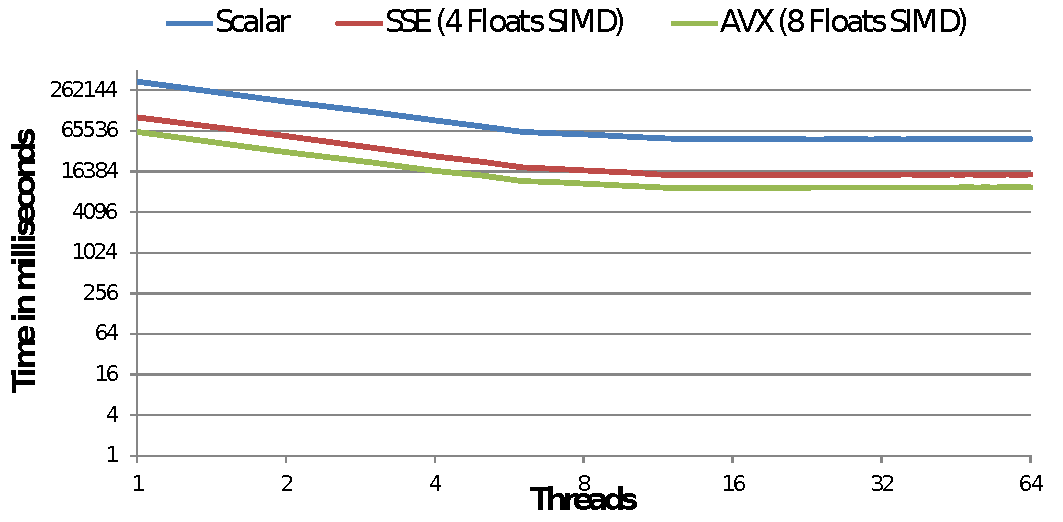
\includegraphics[width = 1.0\linewidth]{figures/cpupoly/Perf_SNB.pdf}
  \caption{\label{fig:PerfSNBTower}
  {Average polygonization time of the towers model when running on SNB processor. Horizontal axis is the number of threads. 
  Vertical axis is time measured in milliseconds.}
}
\end{figure}

\begin{figure}[htb]
  \centering
  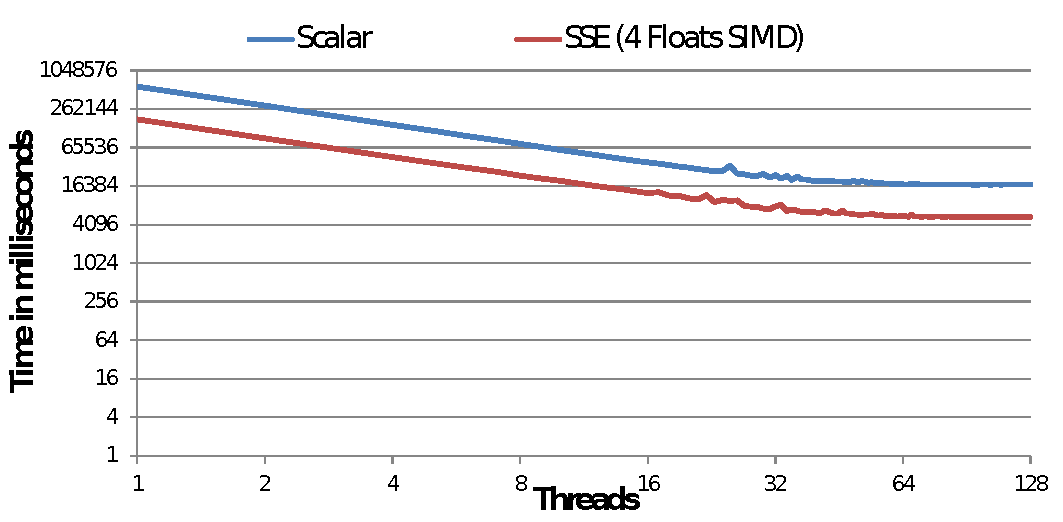
\includegraphics[width = 1.0\linewidth]{figures/cpupoly/Perf_NHM.pdf}
  \caption{\label{fig:PerfXeonTower}
  {Average polygonization time of the towers model when running on NHM processor. Horizontal axis is the number of threads. 
  Vertical axis is time measured in milliseconds.}
}
\end{figure}

%\begin{center}
\begin{table}[H]
\begin{center}
\caption{\label{table:speedup}{Comparison of speedups and field value evaluations per triangle (\textit{FVEPT}) for polygonization of Tower model 
  with different SIMD instruction sets. Note that FVEPT was 17 before adding SIMD optimizations.}}
  \begin{tabular}{ | l | c | c | c | }
    \hline    
    Processor & SIMD Method & Speedup & FVEPT \\ \hline \hline    
    SNB & SSE & 4.58x & 4 \\ \hline
    SNB & AVX & 7.35x	& 2 \\ \hline
    NHM & SSE & 4.25x & 4 \\    
    \hline
  \end{tabular}
  	
\end{center}
\end{table}
%\end{center}

Table \ref{table:speedup} shows the effect of using SIMD optimizations in our algorithm. With SSE and AVX the theoretical speedups are 4 and 8 times, 
respectively. Due to memory alignment techniques and proper caching mechanisms the speedup with 4-wide SSE is greater than 4. The AVX speedup can be 
improved more once scatter/gather instructions are implemented on the SNB processors which will improve the performance of surface extraction algorithm.
Number of field evaluations per triangle shows the average amount of times the field evaluation kernel called to compute a single vertex in the output mesh. 

In another experiment we studied the effect of our early discard method when the side of each \textit{MPU} is less than one 
(figure \ref{fig:DiscardEffect}). Starting from a large cellsize, we reduced the cellsize in uniform steps and measured the polygonization time. 
The red curve shows the polygonization time when the discard method described in section \ref{sec:surfaceextraction} is not being used and the blue curve 
is the timing when that method is in effect. Note that with the blue curve as soon as the \textit{MPU} side is less than one; (\textit{cellsize} = 0.14) empty 
\textit{MPU}s started to get discarded efficiently thus the constant part of the time value is reduced at that point.

\begin{figure}[htb]
  \centering
  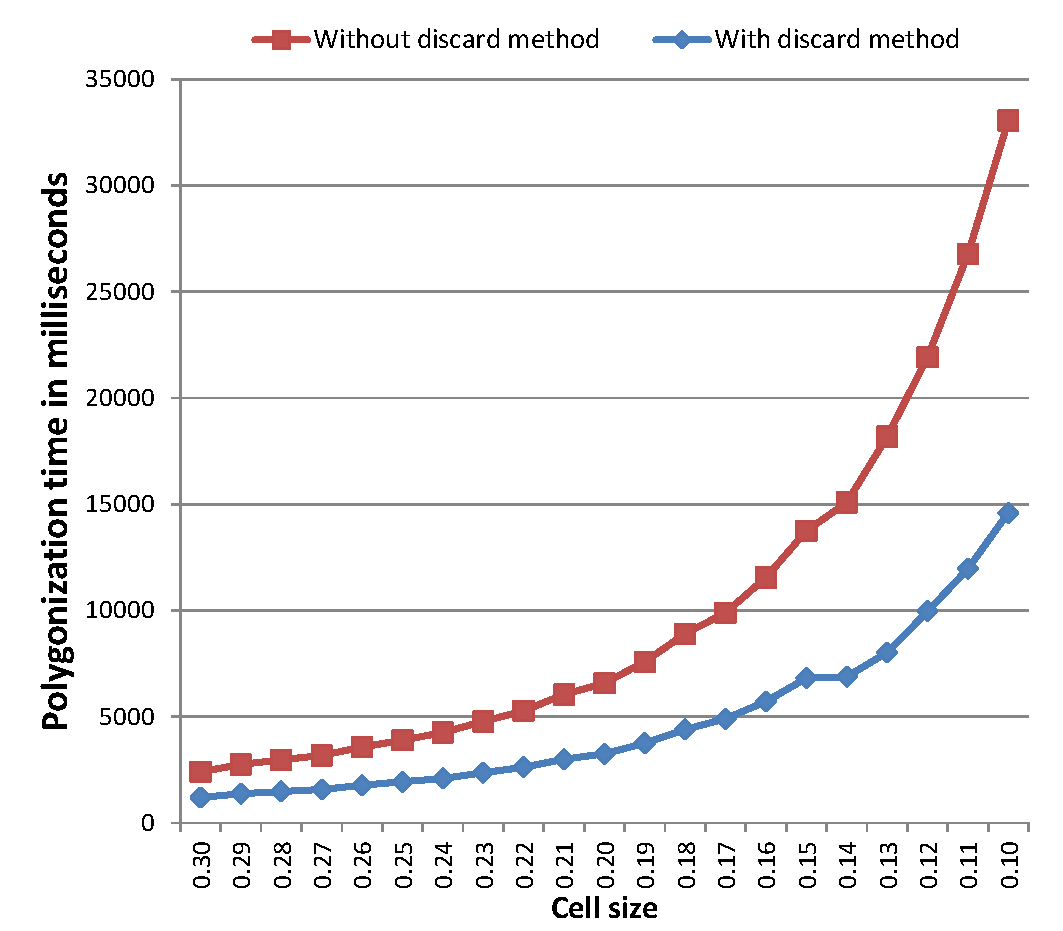
\includegraphics[width = 1.0\linewidth]{figures/cpupoly/DiscardEffect2.pdf}
  \caption{\label{fig:DiscardEffect}
  {Reducing cellsize parameter results in more \textit{MPU} generation and increase in polygonization time.
  However, at a certain cellsize our early discard method stops polygonization time increase by rejecting 
  all empty \textit{MPU}s more efficiently.}
}
\end{figure}



%\ref{fig:ResultScaleSNBTower}, \ref{fig:ResultScaleXeonTower}
Figure \ref{fig:TowerSNBTimeBreakDown} shows the polygonization time breakdown when rendering the towers model on SNB processor. 
Horizontal axis is the core number for a total of 12 cores on that system. As can be seen from the top of this chart; 
the idle time is very short and the cores are active almost all the time. This shows that the work stealing algorithm scales well. 
190463 \textit{MPU}s are processed and 116723 of them are intersected with the iso-surface (40 percent were empty).
40 percent of the \textit{MPUSET} has been processed in less than 10 percent of the total polygonization time.

\begin{figure}[htb]
  \centering
  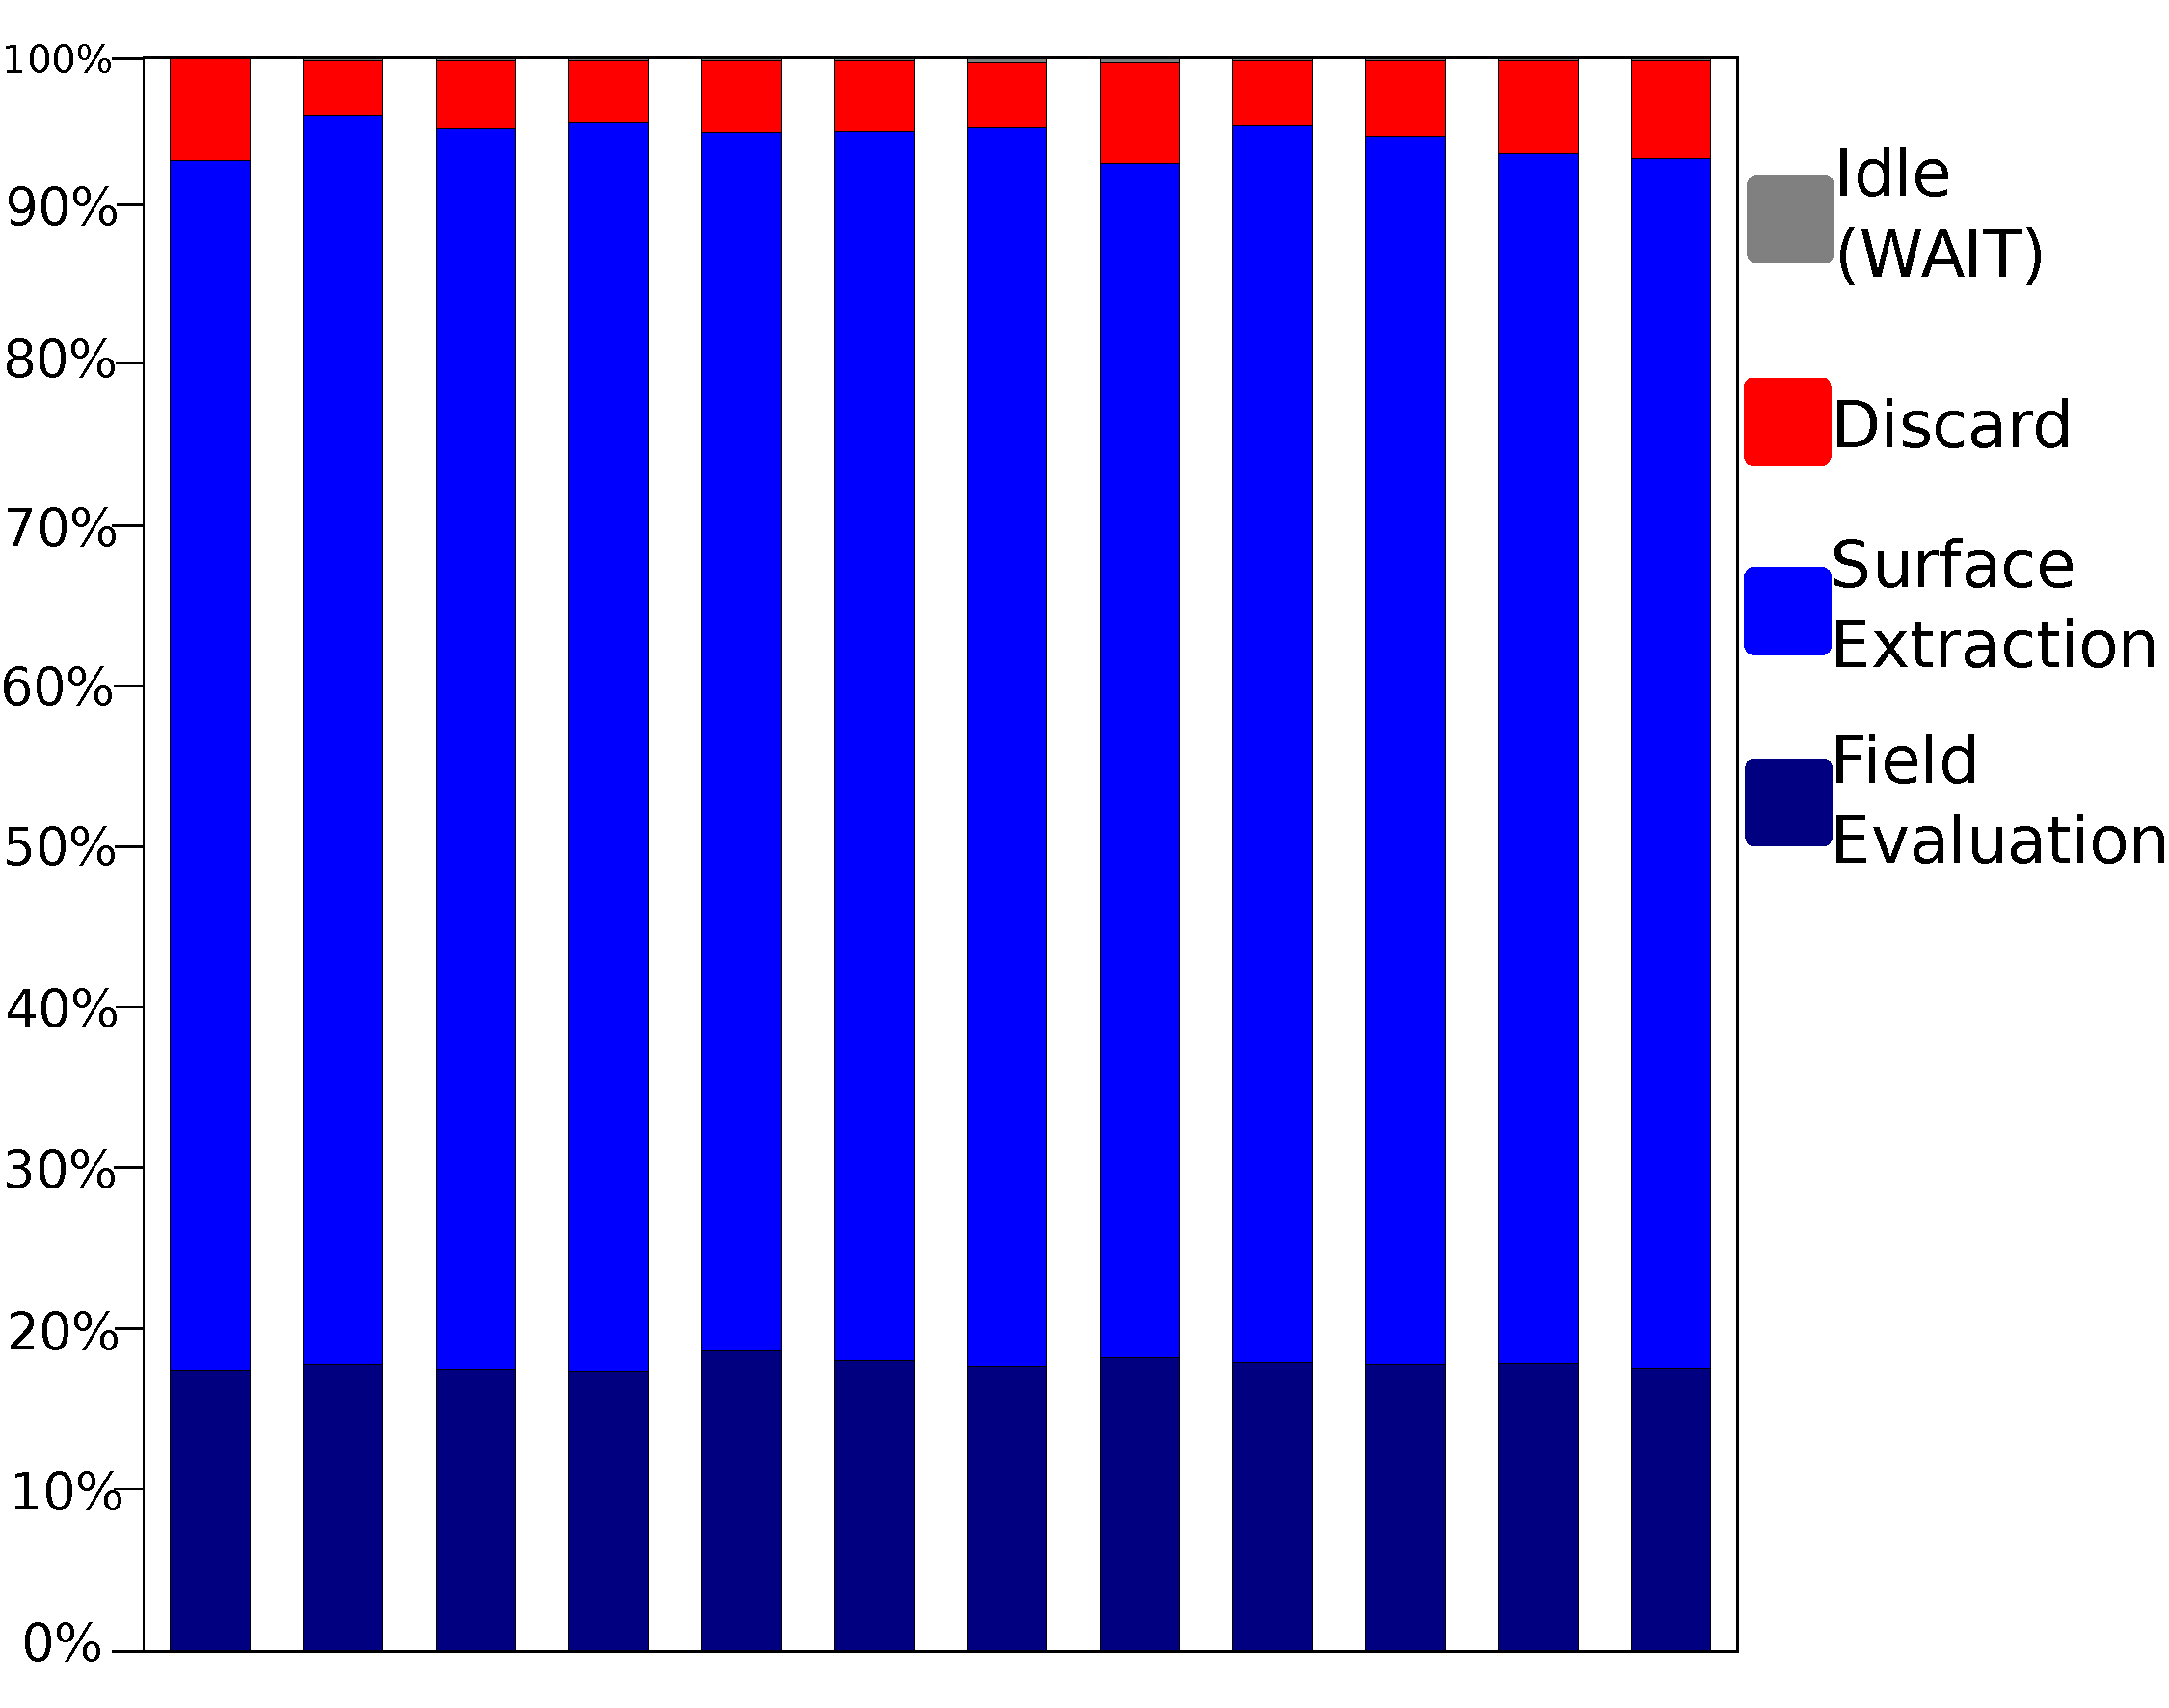
\includegraphics[width = 1.0\linewidth]{figures/cpupoly/PerCoreTimeBreakDown.pdf}
  \caption{\label{fig:TowerSNBTimeBreakDown}
  {Towers model per-core time breakdowns. Each bar represents a logical core on the processor for a total of 12 cores. 
  Vertical axis is the total polygonization time. 190463 \textit{MPU}s processed with 12 cores in 9283 milliseconds. 
  This chart shows the portion of time spent in each step of the algorithm when rendering the towers model on the 
  SNB processor with 8-wide AVX instructions.}
}
\end{figure}

\begin{figure}[htb]
  \centering
  % the following command controls the width of the embedded PS file
  % (relative to the width of the current column)
  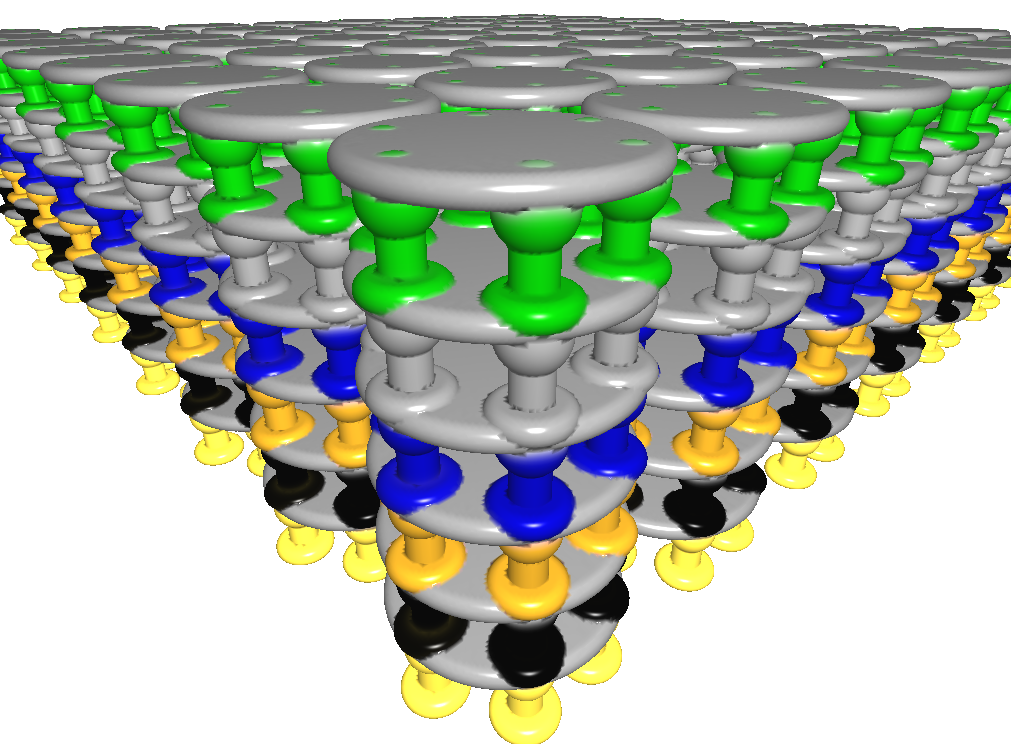
\includegraphics[height = 0.8\linewidth]{figures/cpupoly/towers64}
  \caption{\label{fig:ModelTower}
  {Towers model created with skeletal primitives and binary operators in 
  our incremental designing system. The model is a grid of 8 by 8 towers for a total of
  7360 operators and 7296 primitives.}
}
\end{figure}

\begin{figure}[htb]
  \centering
  % the following command controls the width of the embedded PS file
  % (relative to the width of the current column)
  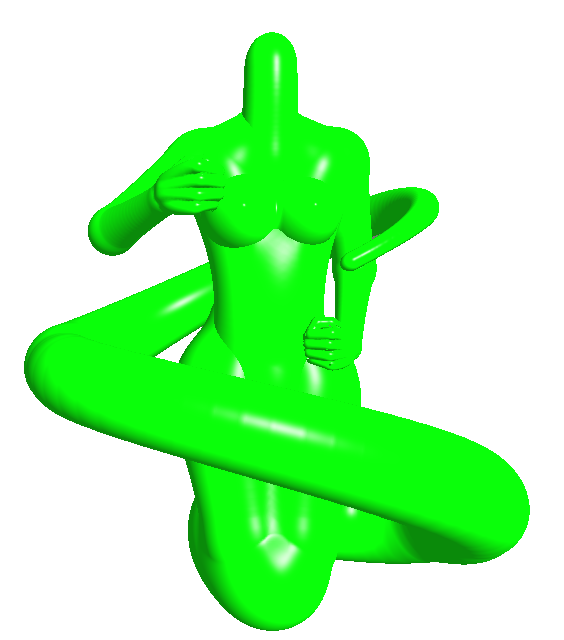
\includegraphics[width=0.7\linewidth]{figures/cpupoly/medusa}
  \caption{\label{fig:ModelMedusa}
  {Medusa model courtesy of Schmidt \etal \cite{SWG2005}.}
}
\end{figure}

These results demonstrate the scalability of our algorithm both in the number of SIMD vector lines and 
the number of cores available on each processor. 

Finally, we compare our method against Schmidt \etal's \cite{SWG2005} using the Medusa model provided by them   
which has 2920 primitives and 11 operators and the tree structure has a depth of 6 (figure \ref{fig:ModelMedusa}).
In this experiment, we divided polygonization timings reported in \cite{SWG2005} by 8 as the best AVX
optimized version of Schmidt's method. Then we ran our polygonization algorithm
optimized with AVX instructions on a single core for Medusa model (See table \ref{table:stats}). 

\begin{table}[H]
\begin{center}
	 \caption{\label{table:stats}
  {Comparison of our polygonization method against Schmidt \etal's \cite{SWG2005} 
  when rendering Medusa model at 5 different resolutions on one single core with AVX instructions. 
  All timings are in milliseconds.}
}
  \begin{tabular}{ | c | c | c | c |}
    \hline    
    CellSize & Our method & Schmidt's method & Speedup \\ \hline \hline
    0.01 & 5220 & 6228 & 1.19x\\ \hline
    0.03 & 3441 & 3653 & 1.06x \\ \hline
    0.05 & 1071 & 2175 & 2.03x	 \\ \hline
    0.10 & 264 & 1292 &	4.89x \\ \hline    
    0.14 & 108 & 721 & 6.67x \\        
    \hline
  	\end{tabular}
\end{center}
\end{table}


The results shows that our algorithm outperforms that of Schmidt \etal by a factor of 6 when running on a single core in lower resolutions. 

\section{Chapter Conclusions}\label{sec:futurework}
In this chapter we presented a new parallel polygonization algorithm using SIMD processing techniques that takes advantage of 
a multi-core machine. Our main contribution is a scalable algorithm both in terms of the number of cores available on 
multicore architectures and the number of SIMD vector width as shown in the results section.  We also presented a SIMD technique for 
finding the intersection of an iso-surface and a cube edge.

%\section{Acknowledgement}
%We would like to thank Intel Corporation for their support and providing us with their cutting-edge server and processors.
%This work is partly supported by the GRAND NCE foundation of Canada, and the Natural Sciences and Engineering Research Council of Canada.

	\startchapter{GPU discretization}
\label{chapter:GPUDiscretization}
In the previous chapter we presented an algorithm for fast triangle mesh extraction from \blob scene graphs. The output of that 
algorithm is a list of vertices with their associated attributes such as position, color and normal and a list of triangles that
defines the connectivity of the surface mesh. While the surface mesh is used for rasterization it can also facilitate  
collision detection and contact modelling algorithms as we will see in the following chapters.  In this chapter we propose an improved 
version of that algorithm that can take advantage of the processing capabilities of the GPU and provides real-time \blob rendering performance. 

Building on top of the results from our SIMD polygonization algorithm, in this chapter we present our work in optimizing that 
algorithm for many-core architectures such as GPU. When compared to the related work in the field, our proposed method has the following
benefits:

\begin{itemize}
 \item It is data-driven, i.e. the input to our algorithm is a dynamic \blob structure that can change 
 in every frame. This is a key advantage that can enable interactive modelling sessions in an implicit 
 framework, i.e. the result of modifications to the model can be viewed in real-time.

 \item The proposed GPU-based data-structure is compact enough to enable rendering complex \blob models 
 in the order of 60,000 nodes. (64,000 nodes only requires about 20MiB of video memory in our system).
\end{itemize}

The data-structure and algorithm are explained in the following sections. The chapter concludes with 
the results and analysis.

%Another requirement for the tetrahedral mesh generation is that the triangular surface mesh should be the boundary surface of the tetrahedral mesh. This is needed since 
%after applying the displacements to the volumetric tetrahedral elements the surface vertices should be displaced as well.
\section{Many-cores architectures}
The advent of programmable graphics pipeline stages opened up new avenues to exploit computational resources of the
GPU hardware. Before the introduction of general-purpose GPU (GPGPU) programming languages, such as open compute language (OpenCL), 
researchers in the field were forced to use computer graphics shading languages (e.g. glsl, cg) to gain access to 
the many-core architecture of GPUs. 

Many of the terms associated with solving rendering issues were borrowed to explain solutions to problems in 
other domains of science. Terms such as vertex, fragment and texture which define entities in a graphics 
shading problem were used to refer to the processing threads, workitems and the input for a solution to a 
problem in high performance computing domain. In addition to the lack of a general language for computing on the GPUs, 
the complexity of mapping the problem domain to the graphics pipeline complicated the implementations and lead 
to various ad-hoc solutions to the same problems. For instance, Georgii \etal created an interactive cloth simulation 
by implementing a mass-spring system using fragment shader programming on an ATI X800 graphics card \cite{Georgii2005}. 
As another example Sorensen \etal reviewed several techniques for accelerating linear system solving
with applications in surgical simulation \cite{Sørensen2006a}. 

At the time of this writing, the following languages are commonly used for GPGPU computing:
\begin{itemize}
 \item Nvidia CUDA (Compute Unified Device Architecture)
 \item Microsoft's DirectCompute
 \item OpenCL which is a standard language maintained by Khronos Group
\end{itemize}

Among all, OpenCL is the only language that is designed to be platform and 
host operating system independant, DirectCompute supports all hardware vendors
but is limited to Windows and CUDA is only available on Nvidia's hardware. 

OpenCL and CUDA share similar concepts in their programming model \cite{gaster2012heterogeneous}.
One of the major drawbacks of OpenCL when compared to CUDA is the initialization delay 
associated with the kernel compile process at runtime. The delay is significant for long
and complex kernels and at the time of this writing, no offline compiler is offered by Nvidia
to alleviate this issue. One way to improve this is to compile and store the binaries 
on disk upon the first kernel invocation and reuse the precompiled binaries for subsequent 
executions. 

The other technical issue that we faced with OpenCL is that the performance optimizations 
made on one platform are not transferred to other platforms. This situation has been experienced
by other researchers in the field and essentially there is no guaranteed portability for the 
tuning and optimizations of the kernels.

The algorithms that are presented in this chapter are implemented using OpenCL. 




\section{Data Structures}
\label{sec:datastructure}
The \blob linearization step introduced in (section \ref{sec:linearization}) is modified to create a compact representation of the input model in our 
GPU polygonization algorithm. 

All the structures are aligned at 16 bytes (four floating points) memory addresses (This is similar to the texture 
accessing techniques in graphical shader programming languages such as (GLSL or Cg) where four floats represent the 
RGBA values of a texel accordingly.) If a primitive node has an associated transformation node with a non-identity 
transformation matrix, that matrix will be stored in the primitive matrices section of the input structure and an 
associated identifier (id) will be provided to the primitive. The default id is 0 which points to an identity transformation 
matrix. The inverse of the primitive matrix is computed and the first three rows of it will be stored for further field 
computations. To transform the axis-aligned bounding boxes of the primitives the full forward transformation matrix will 
be stored in the box matrices section of the structure and it can be accessed using the same id provided for the primitive matrix.
Figure (\ref{fig:datastructure}) depicts this pointerless representation in details.

\begin{figure}[H]
  \centering
  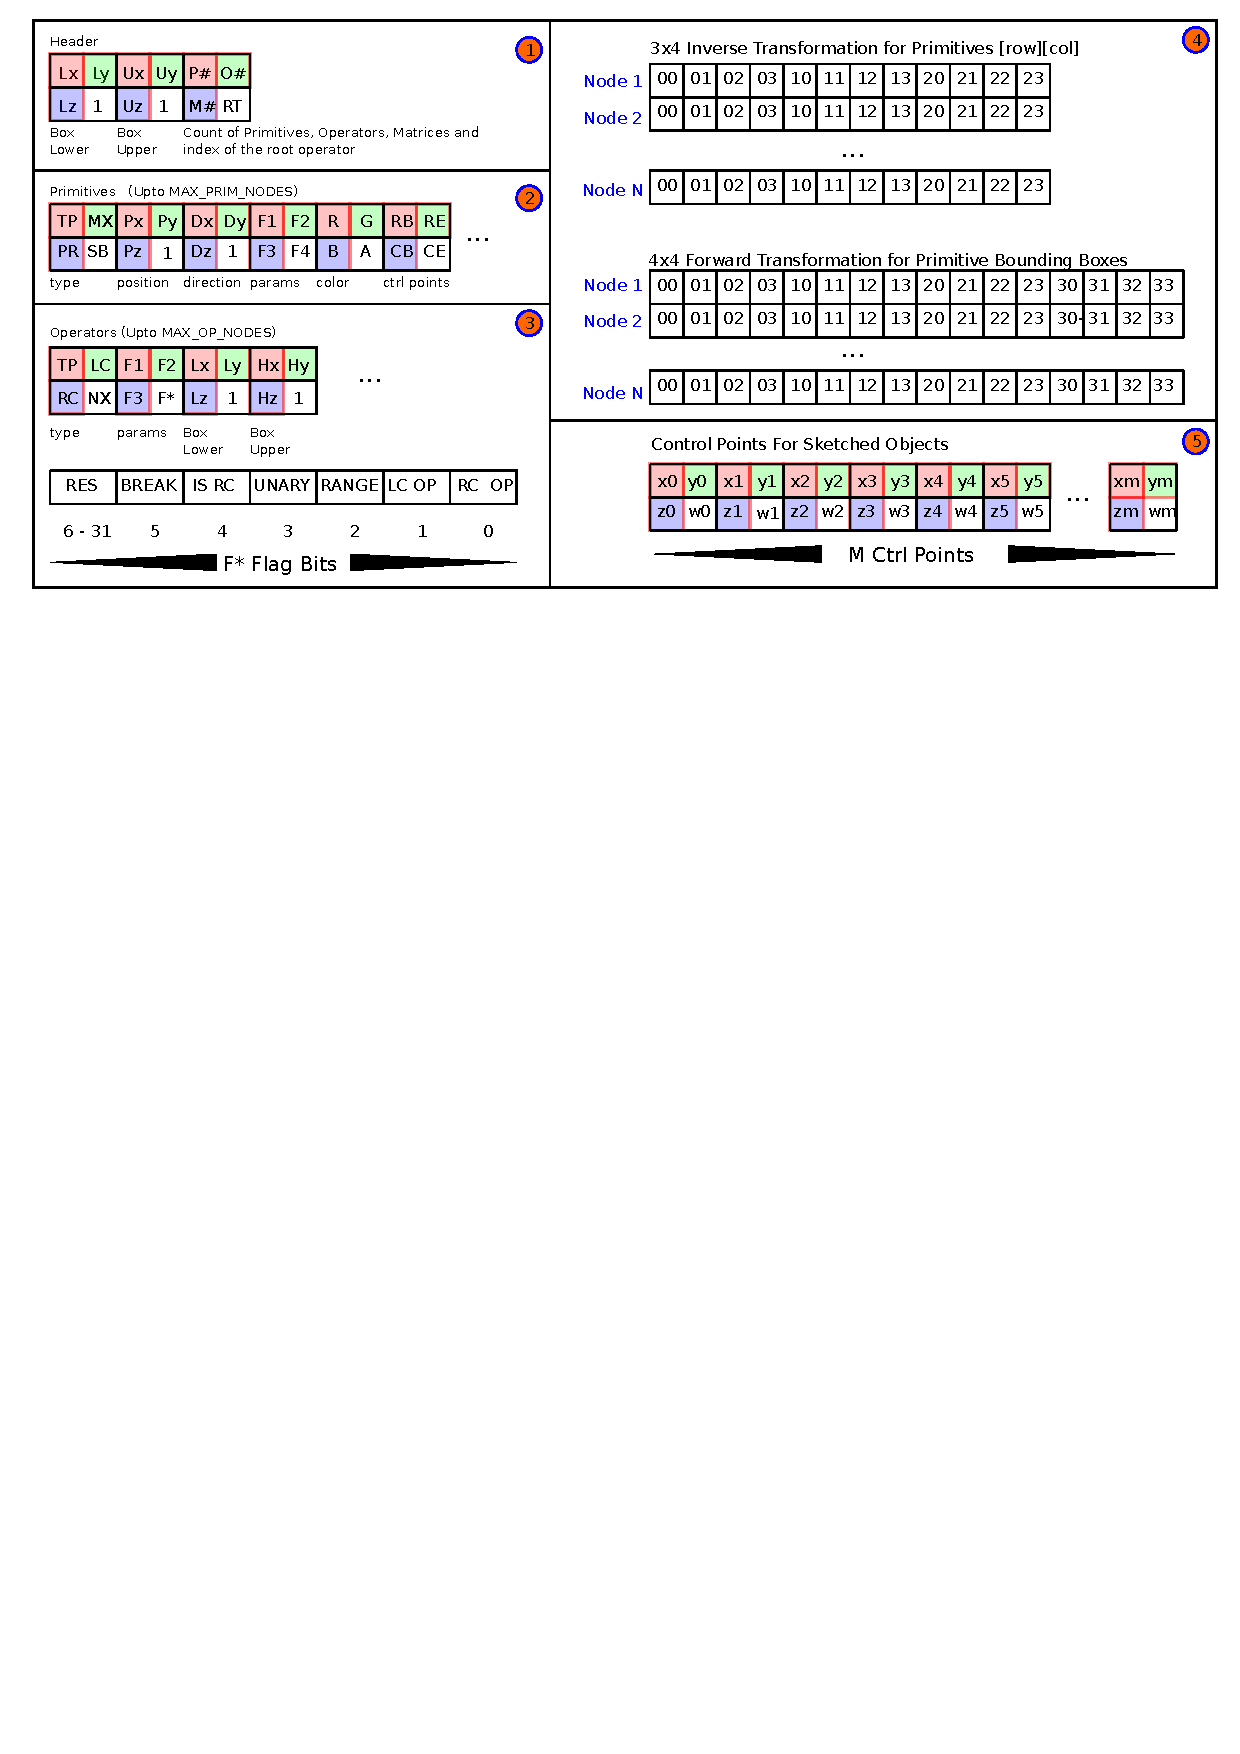
\includegraphics[width=1.0\linewidth]{figures/gpupoly/lineartree.pdf}
  \caption{\label{fig:datastructure}
  {The compact \blob scenegraph representation for GPU polygonization and tetrahedralization algorithms. The structure is 
  aligned at 16 bytes (4 floats). 1- The header. 2- Skeletal implicit primitives. 3- Operators. 4- Affine transformation 
  nodes. 5- Control points for sketched objects. Refer to section \ref{sec:datastructure} for details.}
}
\end{figure}

Each input data-structure is numbered in figure (\ref{fig:datastructure}) for further reference. We review the details in the following:
\begin{enumerate}
 \item The header section defines the lower and upper corner of the axis-aligned bounding box enclosing the entire model, 
 i.e. the convex hull of the input \blob. The header also contains the count of primitives, operators and the transformation 
 nodes. The id associated with the root operator of the tree is also defined in the header.
 
 \item The definition of each primitive is encoded in 6 texels. The $TP$ field in the first texel numerically encodes the 
 type of skeletal primitive. The other three fields in this texel are $MX$, $PR$ and $SB$ that link this primitive to its inverse 
 transformation matrix, the parent and the sibling elements respectively. The following texels define the position, 
 direction, skeleton-specific parameters and the color of the primitive. For the primitives that are 
 computed from sketched control points (e.g. the thin-plate spline primitives \cite{Turk1999, Grasberger}) the indices to the 
 associated first and last control points are stored in the last texel.

 \item A \blob operator is defined in 4 texels. The type of the operator is defined first in the $TP$ field. 
 The following fields define the left and right children, in case all the children are primitives and their indices are in 
 consecutive order (e.g. a range); $LC$ and $RC$ are the indices to the first and last children respectively. This situation 
 can happen if an operator is applied to a list of consecutive primitives, e.g. a global union operator.  The $NX$ 
 field is related to our stackless \blob traversal algorithm which is explained in the following sections and defines the next 
 operator node in the \blob traversal route. The operator-specific parameters and its axis-aligned bounding box are stored next. 
 The $F^*$ flag provides more control over the operator and the definition of its bits can be found at the bottom of figure
 \ref{fig:datastructure}. Bits 1 and 0 are set in case the left child or the right child of the current node are operators as well. Bit 2 is 
 set if the $LC$ and $RC$ indices are actually defining a range of skeletal primitives as explained earlier. In this case the 
 first two fields will be set to zero. If the unary flag is set then the operator has only one child which stored in the $LC$ field.  
 Bit 4 is set when the current operator appears as a right node for its parent. Bit 5 is the break route flag and is discussed further 
 in our stackless \blob routing algorithm. The rest of the bits are reserved for future use. 
 
 
 \item As mentioned above the inverse of the transformation matrices are computed and the first three rows are stored in our input 
 structure for field computation purposes. The elements are depicted in the format of [row][column]. The forward transformation is 
 stored as a 4x4 matrix in a separate input structure for performance reasons. 
 
 \item The control points associated with the sketched primitives are all stored in this section. Each control point is defined with 
 their XYZ coordinate and an associated weight value. 
\end{enumerate}

\section{Memory foot prints}\label{sec:memory}
After analyzing the performance of our OpenCL kernels, register spilling often found to be the major cause for many latencies. Resorting to shared memory spaces, reducing 
number of intermediate variable in field-evaluation kernels and avoiding loop unrolling in some cases helped to optimize the performance. Upon every
change in the input \blob the scene-graph is compacted and transferred from main memory to the GPU. Currently the maximum number of nodes is set at 64K which covers
all of the complex cases we modelled for this thesis. However, for larger \blob models  we can easily increase this amount to support them. The memory footprint of 
our current \blob representation is summarized in table \ref{table:memfootprint}. Each row in the table represents a \blob with a specific number of nodes.
Starting from the simplest \blob with only one node (e.g. a sphere primitive) to the most complex \blob with one million nodes. The middle columns in the 
table are the break down of the required memory size per each component in the compacted \blob data structure.

\begin{table}[H]
\begin{center}
	 \caption{\label{table:memfootprint}
  {Memory footprint of the input \blob in our GPU polygonization algorithm in bytes. The entire \blob for a model with 64K nodes (primitives and operators) 
  takes about 20MB in our current system.}
}
  \begin{tabular}{ | c | c | c | c | c | c | c | c |}
    \hline    
    Nodes & Header & Primitives & Operators & Prim Mtx & Box Mtx & Ctrl Points & Total \\ \hline \hline
    1 & 48 & 96/Prim & 64/Op & 48/Prim & 64/Prim & 16/Point & 320 \\ \hline
    1K & 48K & 96K & 64K & 48K & 64K & 16K & 320K \\ \hline
    64K & 3072K & 6144K & 4096K & 3072K & 4096K & 1024K & 20M \\ \hline
    1M & 48M & 96M & 64M & 48M & 64M & 16M & 320M \\ 
    \hline
  	\end{tabular}
\end{center}
\end{table}


\section{Stackless \blob traversal}
\label{sec:stackless}
As shown in figure \ref{fig:TowerSNBTimeBreakDown} the major bottleneck of the algorithm presented in chapter 
\ref{chapter:cpuPoly} is the surface extraction process. The expensive operations in that 
stage is the computation of normals and colors which require extra field evaluations and hence performance degradation. 

In this section we describe our novel stackless \blob traversal algorithm. 
Without a stack to be maintained the \blob traversal incurs less memory footprint. When dealing with small 
local memory available per each thread on the GPU this reduction in memory usage improves the performance of the 
running kernels significantly.

In high performance rendering algorithms the use of hierarchical spatial data structures for acceleration reasons 
is common. Vising nodes in such structures requires stack-based traversal algorithms. Unfortunately, even the latest 
GPU architectures are poorly suited for implementing such algorithms. 

A complex \blob scene-graph data structure may contain thousands of primitives and operators which can lead to deep tree structures. 
In the original stack-based traversal algorithm, the fieldvalue evaluation process has two stages: A ``down traversal'' followed by an ``up traversal''. 
During the down traversal stage all operators starting from the root node are visited and pushed onto an operators stack until a leaf node (primitive) 
is reached at which point the field due to the primitive is computed and pushed onto a separate fields stack and the next 
stage which is the up traversal begins.

During the up traversal stage the operators are popped out of the stack and per each child an associated field is popped from the fields stack for the 
operator to combine them in its own specific way. The resulting field is again pushed back on the fields stack.  This process continues until the 
operators stack get emptied and the final fieldvalue due to the root node is computed and returned.

Performing many push and pop operations limit the performance of the traversal process. The other issue relates to the 
inherently dynamic storage requirement for the stack itself. Although, creating a fixed-size stack is possible but since the stack size is a function of
the count of nodes in the input \blob, this will ultimately limit the maximum number of nodes in a complex scene. If $N$ is the maximum number of nodes 
(primitives plus operators) allowed in a \blob model then the minimum number of elements to be stored in the stack during the traversal process 
is given by: $M=\log(N)$ or the depth of the binary tree created by $N$ nodes. Recalling from section \ref{sec:memory} there is a limited amount of
local memory available per each thread executing on the GPU. Keeping the stack in the shared memory will also complicate the implementation and
the access patterns from other threads in the current thread block and may impact the performance. Needless to say that implementing a stack in the global 
video memory will require very expensive memory transfers and is not an option for a real-time rendering algorithm. 


Our algorithm is based on the neighbor cell-links concept in the stackless traversal of spatial subdivision trees 
which is first introduced by Samet \etal \cite{Samet1984,Samet1990}. Using a similar technique Popov \etal presented 
a stackless KD-Tree Traversal for high performance GPU ray tracing algorithm \cite{Popov2007}. 

%Although the \blob traversal algorithm presented here is somewhat different in my approach, a similar idea was put forward 
%by my fellow student, Herbert Grasberger, and submitted for publication. The details to be found in his thesis \cite{Grasberger2015}. 
%The following \blob traversal stage was developed independently inspired by his draft publication.

The algorithm is divided into two stages. A preprocessing stage to compute a traversal route for the entire 
\blob and the GPU-based stackless traversal stage to compute the field-value due to a given point in space. 
The following will describe these two stages in greater details.


\begin{figure}[H]
  \centering
  % the following command controls the width of the embedded PS file
  % (relative to the width of the current column)
  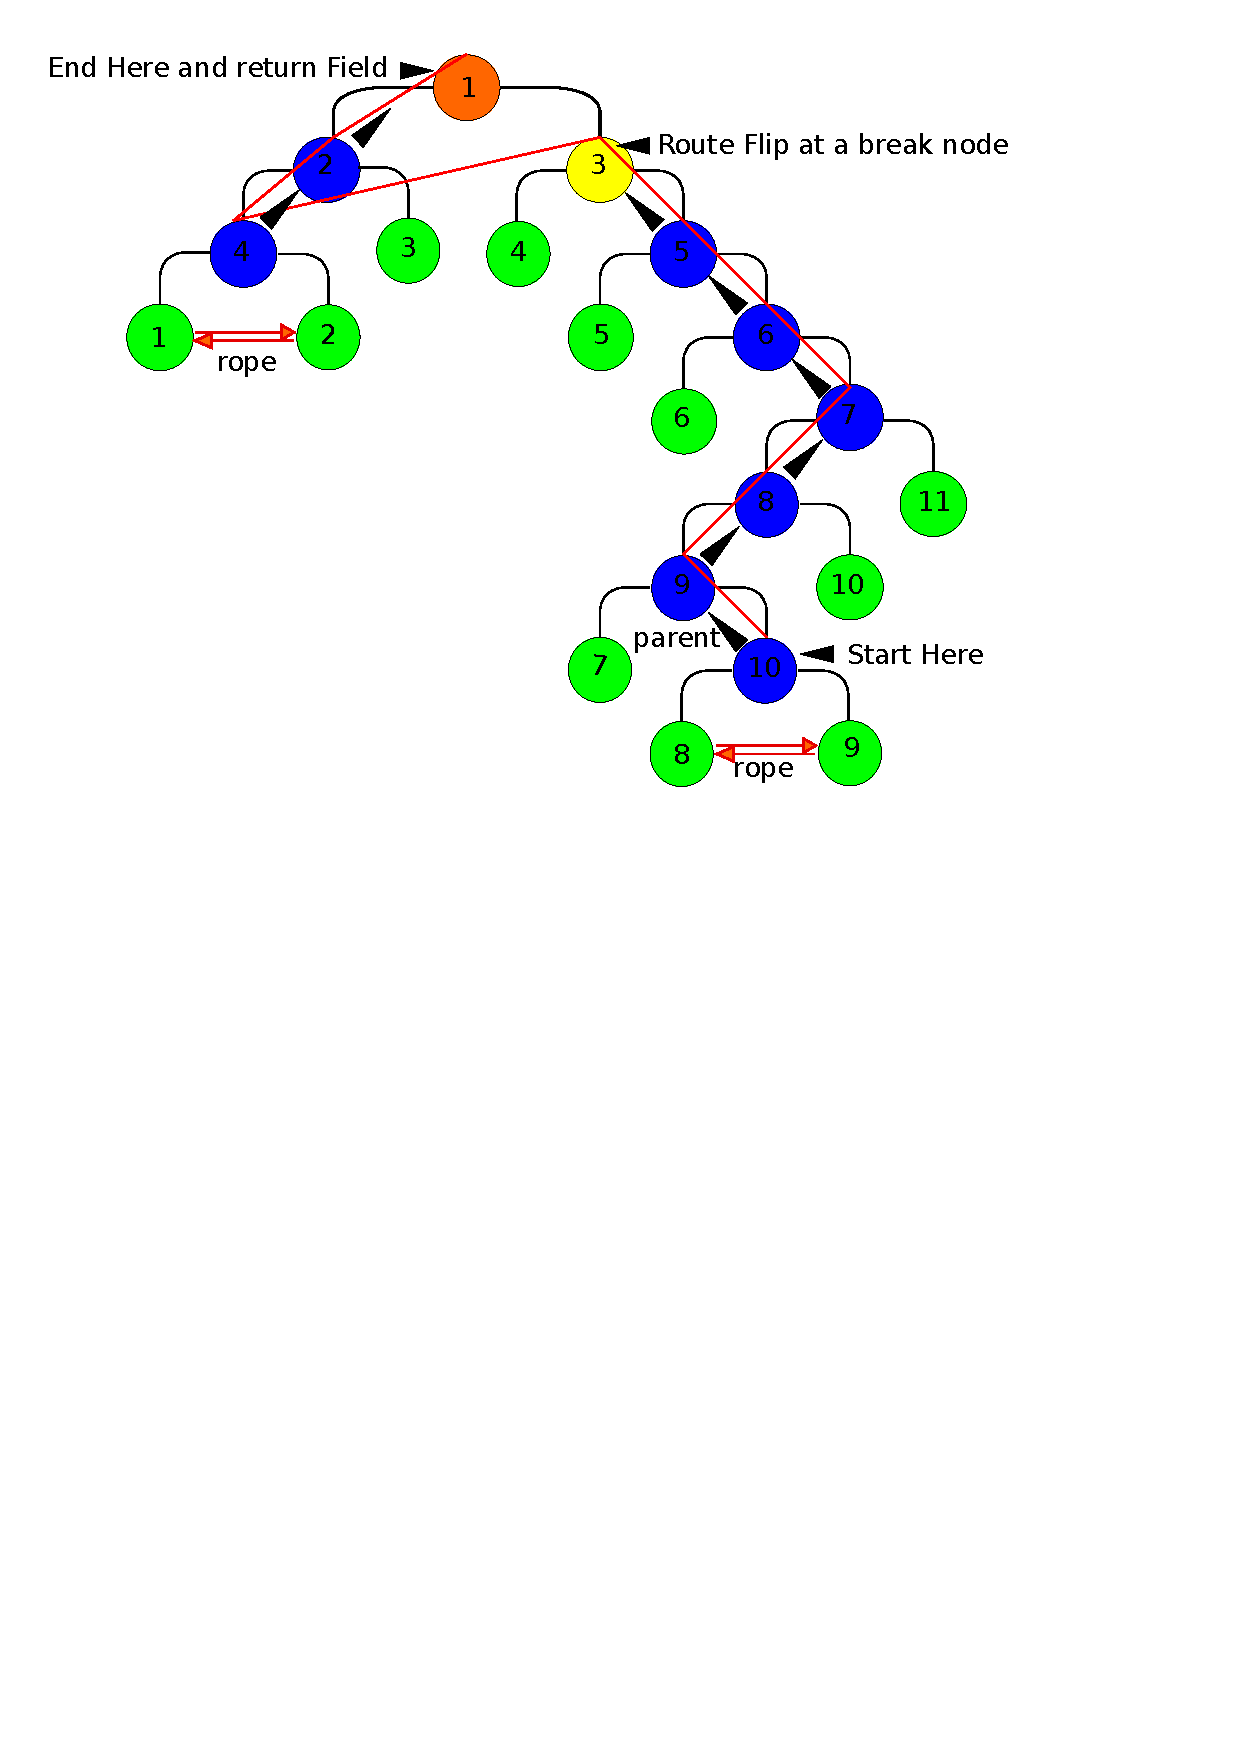
\includegraphics[width=1.0\linewidth]{figures/gpupoly/stackless.pdf}
  \caption{\label{fig:stackless}
  {Stackless \blob traversal algorithm performs faster on deep tree traversals. The route is computed once and encoded into the tree upon transferring the input 
  data structures to the GPU.}
}
\end{figure}

\subsubsection{Encoding traversal route}
The first stage in our algorithm is to compute a route to visit all nodes in the \blob 
and finally encode that route in the GPU input data-structure. This process is performed only once and is not a 
bottleneck in the system. The one-time fixed cost paid for this stage on the CPU is regained 
when many fieldvalue evaluations are performed in parallel on the GPU without the extra cost 
associated with the stack storage.

To compute the route the following steps are performed on the CPU side as a preprocessing stage: 

Using the naive \blob traversal algorithm the nodes are visited from root to leaves. Two stacks are maintained in this process, an
operators stack $S1$ and a \text{break} nodes stack $S2$. The latter is defined in the following:

\begin{enumerate}
 \item If one of the children is an operator $A$ and the other is a primitive $B$. The parent for $A$ is set 
 to the current node and then it is pushed onto $S1$.
 
 \item If both children are operators. The right child is set as a \textit{break} node and is pushed on to $S2$. 
 The route at break nodes is flipped to the left branch of the tree, see figure \ref{fig:stackless}. 
 
 \item If the two children are both primitives: First the root of the \blob is set to the current node if it has not been set before.
  (Refer to the \blob header format in figure \ref{fig:datastructure} for the location of the root field shown as $RT$.) 
  A rope is created between the two primitives, linking the two nodes and a break node $B$ is popped from $S2$. 
  The next node for $B$ is set to the current node.
 
  
 \item This process is continued until $S1$ is emptied.
\end{enumerate}


%add an algorithm listing for this

%describe what happens on the GPU as well

\subsubsection{Up-sweep traversal on the GPU}
Figure \ref{fig:stackless}, shows the final route for a sample \blob. The benefits of this type of routing encoded into the tree
is that there is no need for storing a deep stack to store the intermediate operators. Using this new approach the tree is now only evaluated 
from bottom to top. 

The \blob root node $RT$ marks the starting point of the traversal. This field is stored in the header section of the 
data structure as illustrated in figure \ref{fig:datastructure}. Using the new traversal route this field is set to
the operator node 10 for the example \blob shown in figure \ref{fig:stackless}. 

In case of an operator where all its children are primitives, the field due to each child is computed before the operator evaluation. 
The computed field is stored in the global field variable $F1$ and using the link to the next node provided in the structure ($NX$) 
the evaluation continues to the next operator in the tree at an upper level (up-sweep). When evaluating an operator with one primitive
child then the field due to the primitive child is computed before applying the current operator to $F1$ and performing the up-sweep (nodes 5 to 9 in 
figure \ref{fig:stackless}).

When visiting a break node the field is computed as usual but this time it is stored in the special variable $F2$, instead. 
In addition at a break node, the $NX$ field in the structure points to a non-parent operator (operator 4 for break node 3 in the example).

The process continues until the first node in the tree is evaluated at which the $F1$ and $F2$ values store the children fields for 
their parent. The $NX$ field associated with the first node points to itself which marks the end of the traversal process.


\section{GPU Surface Extraction Algorithm}
\label{sec:surfextraction}
In this section we present our GPU polygonization algorithm which is based on our novel field value evaluation technique described
in the previous section. Since the following steps are implemented using OpenCL on the GPU we will use the term \textit{kernel} which 
is a single thread of execution on the GPU. Please refer to section \ref{sec:memory} for a description of the memory model for
general purpose GPU (\textit{GPGPU}) programming.

We start by computing the axis-aligned bounding box of the model by traversing the tree from root to leaves 
and applying the transformation matrices at leaf nodes (primitives). Using the \textit{cellsize} parameter supplied by the user the 
bounding box is subdivided into a grid of voxels. The kernel \textit{ComputeAllFields} then computes a fieldvalue per each
vertex of the voxel grid and stores that value in the format of \textit{XYZF} where \text{XYZ} denotes the position and 
\textit{F} is the so-called field at that point. 


After computing all the fields, the grid edges are processed in the following order. 
Each vertex in the grid is connected to at most 6 other directly adjacent vertices. Starting from the lower corner of the voxel grid 
the kernel \textit{ProcessEdges} visits the corresponding vertex in the grid and examines only the edges that start 
from that vertex and extend to the adjacent vertices in the next index step. This way all edges in the voxel grid are checked 
and redundant traversals can be avoided. Needless to say that at boundary vertices the kernel may process less than 3 edges per each 
vertex (i.e. the ones that are within the convex-hull of the model). Upon each kernel run at this stage the index address to 
the corresponding vertex and its 3 other adjacent vertices is computed as shown in the algorithm \ref{alg:processedgeskernel}. Per each vertex
an inclusion query is performed (i.e. The fieldvalue at that vertex is compared against the iso-value. If it is greater than or equal 
the isovalue the vertex is considered inside otherwise outside the model). Two values are stored before completion of this kernel call. 
The first is the count of crossed edges at that vertex and the second one is a 3 bits flag which basically locates the intersected 
edges along x, y or z axes.


\begin{algorithm}[H]
\caption{\textit{ProcessEdges} kernel counts the number of intersected edges and their corresponding axes. 
This kernel runs per each vertex in the voxel grid.}
\label{alg:processedgeskernel}
\begin{algorithmic}[1]	
  \STATE $v = queryVertexInclusion(i, j, k)$
  \STATE $vx = queryVertexInclusion(i+1, j, k)$
  \STATE $vy = queryVertexInclusion(i, j+1, k)$
  \STATE $vz = queryVertexInclusion(i, j, k+1)$
  \STATE $count = (v \xor vx) + (v \xor vy) + (v \xor vz)$
  \STATE $flag = (((v \xor vx) << 2) or ((v \xor vy) << 1) or (v \xor vz))$
\end{algorithmic}
\end{algorithm}

In the above algorithm the \textit{queryVertexInclusion} function checks whether the vertex at a specified
voxel grid index is inside the model i.e. the field value at that vertex is greater than or equal to the \textit{isovalue}.
Then it performs the same test for the end-points of the edges emanating from the current vertex along the primary axes.
If both endpoints of an edges are inside (or outside) the model then there is no intersection between the iso-surface and
the voxel grid. Variable $count$ stores the number of intersections associated with the current vertex at the grid address 
$\left(i, j, k\right)$. In addition a 3 bits \textit{flag} variable holds the state of the intersections along the primary 
edges in the format of $XYZ$.

After processing all edges, the array \textit{EdgeBuffer} contains the count of intersected edges per each vertex 
in the voxel grid. In order to compute the total number of output vertices in the triangle mesh the prefix-sum 
\cite{Sengupta2007} of \textit{EdgeBuffer} is computed and stored in a separate gpu memory buffer called 
\textit{ScannedEdges}. The total number of vertices is the sum of the last elements in the \textit{EdgeBuffer} 
and \text{ScannedEdges} arrays. Before computing the vertex attributes such as the position, color and normal, the associated 
memory buffers are allocated on the device using the total number of vertices computed in the previous step. 

After this stage the vertex attributes of the mesh can be computed by executing a root finding method on the intersected 
edges and storing the output vertices in their appropriate buffer locations using the offsets in \textit{ScannedEdges}.
We use a Newton-Raphson root finding method which converges to the iso-surface using the gradient of the field \cite{Matthews1987}.
At each iteration the root is displaced closer to the surface according to the method given by Overveld \etal (\cite{VanOverveld2004}):

\begin{equation}
 r = r + \frac{\left(iso - f(r)\right)}{\nabla V(r).\nabla V(r)}
\end{equation}

Where $r$ is the root, $f(r)$ is the field at $r$ and $\nabla V(r)$ is the gradient of the field at $r$.
A maximum of four iterations was sufficient to provide smooth results in our tests. 
After computing the root position other attributes such as the color and normal at that vertex are also computed and stored in their 
designated buffers. The next step is to process the cells in the voxel grid in parallel and compute a configuration index per each cell
for extracting the topology of the triangles. There is no \blob traversal at this stage since the computed fields will be provided
to the kernel function. The configuration table is supplied as a texture and can be accessed using sampler unit for 
fast access. The number of triangles that are output per each cell is stored in a buffer called \textit{FaceBuffer}.

In order to find the total number of triangle elements, a prefix-sum scan is applied to the \textit{FaceBuffer} array 
in the same way that total number of vertices is computed previously. The buffer \textit{ScannedFaces} will be used to hold the 
offset values per each cell. 

The final stage in our GPU polygonizer is producing the triangles. For this purpose the kernel function \textit{GenerateFaces} 
is called per each cell in the voxel grid. No \blob traversal is required for this stage. Only the cells which intersect with the 
iso-surface are processed. Upon each kernel run the indices for the eight vertices of the current cell are computed. 

To process cell configurations we used the improved marching cubes table by Dietrich \etal 
\cite{Dietrich2009}, which avoids most of the small and badly shaped triangles. The table is supplied to the kernel as 
a texture of size 256 rows by 16 columns. To access the entries in the table the texture sampler on the hardware 
can be used. Per each cell the configuration index is computed using the previously stored fields. Each entry in the table is the 
index of an edge in the cell (There are 12 edges per each cell). Algorithm \ref{alg:generatefaceskernel} shows how the 
triangle elements are computed in this stage.

\begin{algorithm}[H]
\caption{\textit{GenerateFaces} kernel function computes the triangle indices per each cell and outputs them directly into an
OpenGL index buffer for rasterization. All the buffers can be read back from the GPU and stored.}
\label{alg:generatefaceskernel}
\begin{algorithmic}[1]	 
  \STATE $index = globalCellIndex(i, j, k, dim)$
  \STATE $config = cellconfig(i, j, k)$
  	  \IF{$config == 0$ or $config == 255 $}
	  \STATE return;
	  \ENDIF	
   \STATE $cellcorners = cellCornerIndices(i, j, k, dim)$
   \STATE $offset = ScannedFaces[index]$
   \STATE $count = FaceBuffer[index]$
   \FOR{$i=1 \to $count}
	 \STATE $edge = sample($configtable$, int2(edge, index))$
	 \STATE $start = EdgeStartIndex[edge]$
	 \STATE $axis = EdgeAxis[edge]$
	 \STATE $elements[offset + i] = ScannedEdges[cellcorners[start]] + axis$
   \ENDFOR				

\end{algorithmic}
\end{algorithm}


Upto five triangles can be extracted from each cell. Lines 11 and 12 in the algorithm assign the start index of an 
edge and its associated axis using two constant buffers supplied to the kernel for this purpose. 
The element entry is computed as an index to the global vertex buffer. The \textit{ScannedEdges} 
buffer holds the global offset for all the intersected edges as previously discussed. 

\section{Analysis and Results}
In this section we review the effects of the previous optimizations on the overall performance of the system.
In our experiments we tested the effect of the stackless \blob traversal algorithm using a set of models created 
with our incremental modelling system. To make a fair comparison the same algorithm implemented on the GPU using
the OpenCL framework once with the stack and the other time with the stackless method presented in section 
\ref{sec:stackless}. The results are shown in the following table:



\begin{table}[H]
\begin{center}
	 \caption{\label{table:stackless}
  {Stackless \blob traversal improved the performance of our \blob field evaluation significantly.
  Here is the comparison between our novel stackless approach versus the stack-based implementation for various models. 
  Timings are the average of 100 runs.}
}
  \begin{tabular}{ | c | c | c | c | c | c |}
    \hline    
    Model Name & Field Queries & Grid & Stack-based (ms) & Stack-less (ms) & Speedup \\ \hline \hline
    Tumor & 16240 & 29*20*28 & 21 & 0.8 & 26x\\ \hline
    cake & 18975 & 33*23*25 & 17 & 1 & 17x\\ \hline
    3slabs & 28750 & 46*25*25 & 30 & 2 & 15x \\ \hline
    \hline
  \end{tabular}
\end{center}
\end{table}


\begin{figure}[H]
  \centering
  % the following command controls the width of the embedded PS file
  % (relative to the width of the current column)
  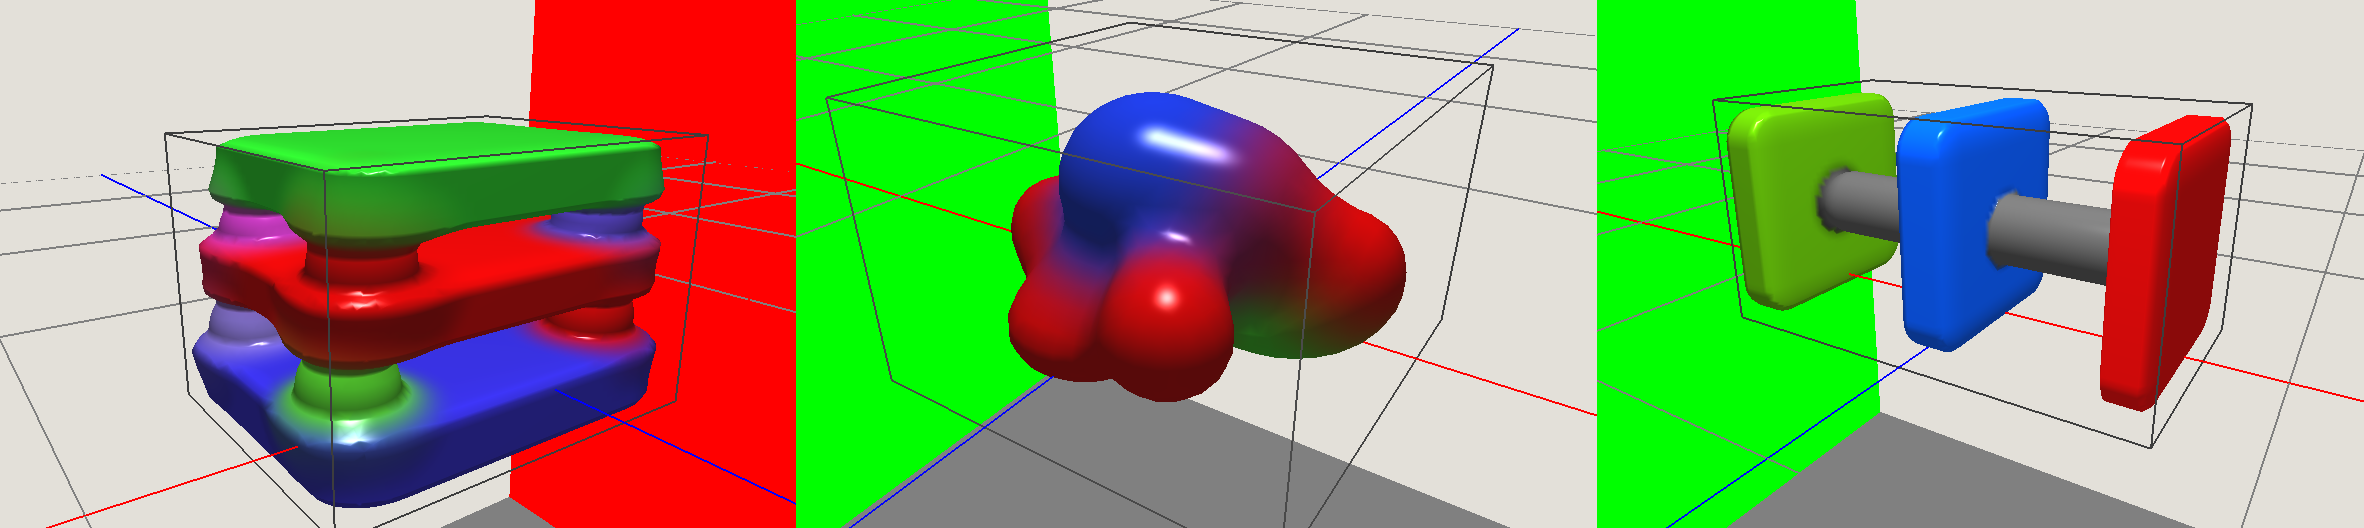
\includegraphics[width=1.0\linewidth]{figures/gpupoly/combined_models.png}
  \caption{\label{fig:combinedmodels}
  {Sample models for testing our GPU polygonization method. From left to right: Cake, tumor and 3slabs.}
}
\end{figure}

When using stacks, the register spilling phenomenon mentioned previously degrades the performance due to the higher cost of accessing 
the shared memory. Conditional push and pops in the stack-based method also stalls the performance of the kernels.  

Faster field evaluations using the stackless algorithm also improves the performance of our root-finding method and the overall
polygonization time. In the following we review per kernel time break-time which provides a close look at hotspots (most time-consuming 
locations) in our implementation. 

%Tumor: Fields: 2, Edge: 1, EdgeBufferScan: 22, Vertex: 44, Cell: 1, FaceBufferScan: 18, Faces: 17, Total: 105
%Cake: Fields: 1, Edge: 1, EdgeBufferScan: 19, Vertex: 58, Cell: 2, FaceBufferScan: 17, Faces: 10, Total: 108
%3Slabs: Fields: 1, Edge: 1, EdgeBufferScan: 18, Vertex: 40, Cell: 1, FaceBufferScan: 17, Faces: 1, Total: 79

\begin{figure}[H]
  \centering
  % the following command controls the width of the embedded PS file
  % (relative to the width of the current column)
  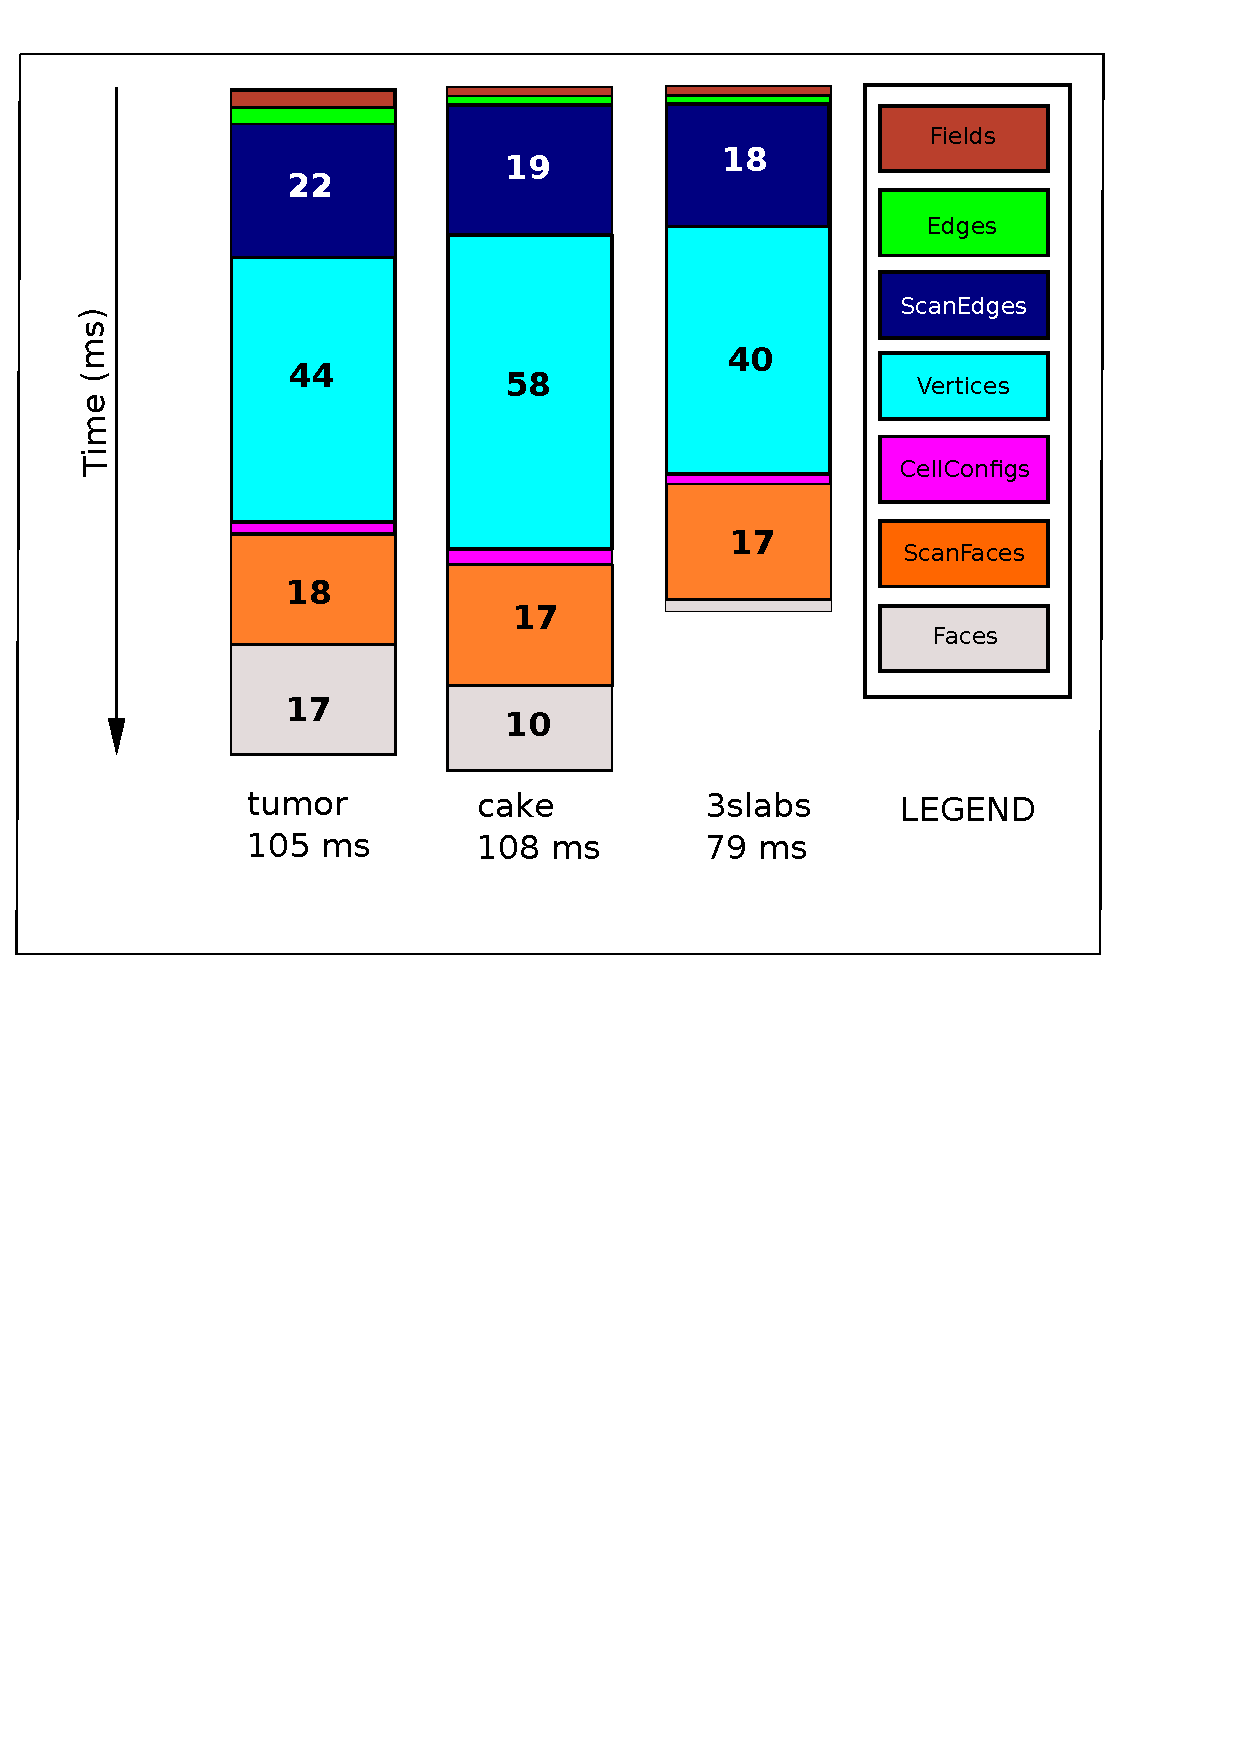
\includegraphics[width=0.8\linewidth]{figures/gpupoly/breakdownpoly.pdf}
  \caption{\label{fig:breakdownpoly}
  {Polygonization time breakdown in milliseconds for the three models shown in the previous section. Vertex processing is the most compute-intensive
  stage due to the Newthon-Raphson root finding method employed and the evaluation of colors and normals which require additional traversals.
  }
}
\end{figure}

As it can be seen computing vertices is still the most time-consuming stage due to the extra tree traversals required for high quality 
gradiant-based Newthon-Raphson root-finding method. Computing other attributes such as colors and normals would also need 1 and 4 
traversals respectively. The prefix-sum scan operator employed here uses multi-pass computing. The extra cost of kernel calls has
increased the cost of using these operators. Several optimizations can be performed to benefit the overall performance. By 
vectorizing all kernels the core SIMD units can be used more efficiently. The prefix-sum scan operator can also be implemented in such a way 
that the memory-bank conflicts are completely avoided and the data-accesses are performed in parallel.























	\startchapter{GPU-Accelerated Finite Element Framework}
\label{chapter:finiteelementmethod}






















        \startchapter{Real-time Cutting}
\label{chapter:Cutting}
One of the main objectives of a virtual reality based surgical simulation system is the removal of pathologic tissue 
\cite{Steinemann, Nienhuys2001a}. Cutting imposes many challenges to the development of a robust, interactive surgical 
simulation, not only because of the nonlinear material behavior exhibited by soft tissue, but also due to the
complexity of introducing the cutting-induced discontinuity. 

We developed our new volumetric mesh cutting system named ``VolCut'' in the context of a human skull craniotomy simulation. When an abnormality of the brain is suspected, 
Stereotactic \footnote{Stereotactic surgery or stereotaxy is a minimally invasive form of surgical intervention which makes use of a three-dimensional 
coordinate system to locate small targets inside the body and to perform on them some action such as ablation, biopsy, lesion, injection, stimulation, 
implantation, radiosurgery, etc.} brain needle biopsy is performed and guided precisely by a computer system to avoid 
serious complications. A small hole is drilled into the skull, and a needle is inserted into the brain tissue guided by computer-assisted 
imaging techniques (CT or MRI scans). The actual biopsy process can not be seen by the surgeon. For this reason,
non-progressive cutting, where a tetrahedral element is decomposed after the sweep surface traverses the tetrahedral elements, is a reasonable
approximation for that application. Also, in the current stage of our system, we do not model any haptic interaction of the cutting tool with the 
deformable object during a cut. 


\section{Overview}
The physics simulation in VolCut uses tetrahedral meshes to compute deformations. In this section,
we present our GPU-assisted approach to cutting tetrahedral meshes in real-time. 
The input to VolCut is a cut trajectory and an edge-based data structure representing the tetrahedral mesh. 

The tetrahedral mesh itself is extracted from the \blob model that is created using the incremental modelling 
system described in section \ref{sec:implicitmodellingintro}. The complete process is summarized below:

\begin{itemize}
 \item The user models the elastic tissue using the \blob approach (section \ref{sec:implicitmodellingintro})
 \item The proposed GPU-accelerated polygonization algorithm provides real time updates for the modifications 
 that are made to the model throughout the design process (section \ref{sec:surfextraction})
 
 \item The final model is converted to a tetrahedral mesh with the algorithm presented by Si \etal \cite{Si2006a}.
 This is a one-time process and is not a bottleneck in the system. The triangle mesh extracted in the previous stage is 
 used as an input to the tetrahedralization algorithm. The output is a volumetric tetrahedral mesh. 
 
 \item Our physics simulation handles the dynamic behavior of the model and handles the collisions with other
 objects in the environment including the scalpel. 
\end{itemize}


As shown in figure \ref{fig:sweepsurf}, the user moves the cutting tool and the system records the path of the 
blade endpoints shown in purple. The first intersection between the recorded trajectory and the model marks the 
beginning of the cutting process. When the tool completely traverses the model the system computes the cutting
configurations as described below. 

\begin{figure}[H]
\centering
\begin{subfigure}{.5\textwidth}
  \centering
  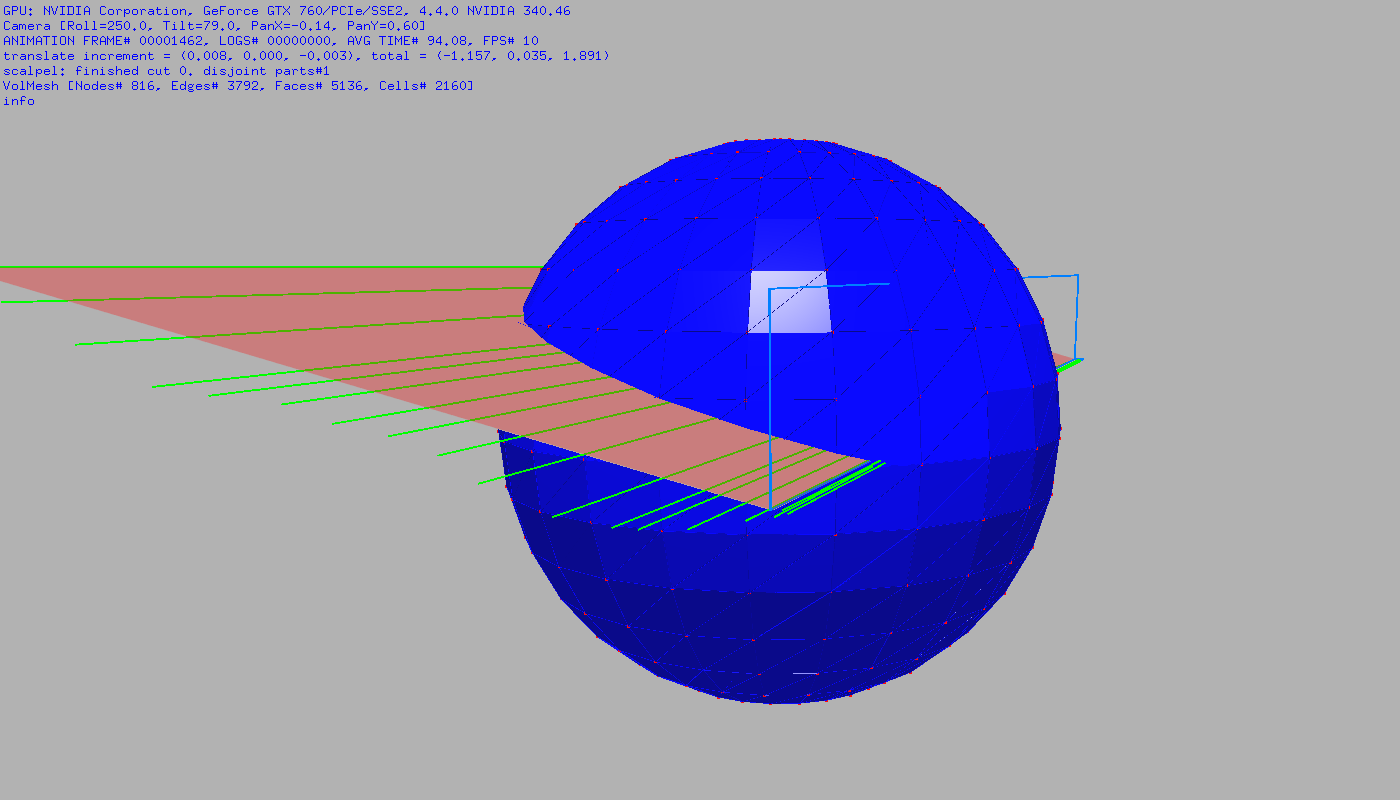
\includegraphics[width=0.8\linewidth]{figures/cutting/trajectory03.png}
  \caption{The trajectory of the cutting tool}
  \label{fig:sub1}
\end{subfigure}%
\begin{subfigure}{.5\textwidth}
  \centering
  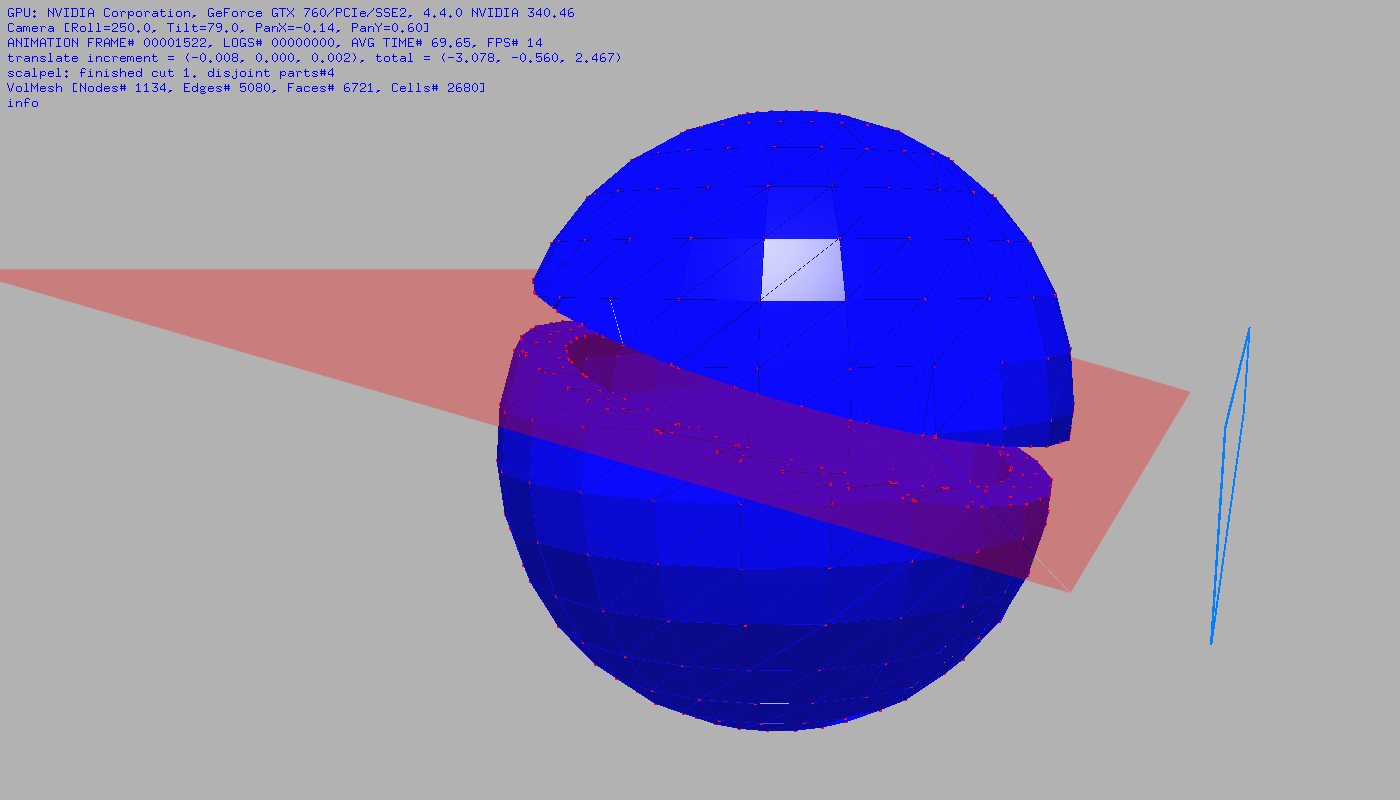
\includegraphics[width=0.8\linewidth]{figures/cutting/trajectory04.png}
  \caption{The shell model after cut}
  \label{fig:sub2}
\end{subfigure}
\caption{The cut trajectory in blue and the sweep-surface shown in pink. The scalpel passes through the shell model for cutting.}
\label{fig:sweepsurf}
\end{figure}


The following steps are performed to complete the cut induced by the scalpel on the mesh:

\begin{enumerate}
 \item Using the GPU-accelerated algorithm described in section \ref{sec:CuttingEdgeIntersections}, the intersection of the 
 sweep-surface and all the edges of the mesh are computed. The output of this stage is a list of cut-edges and their associated 
 intersection points. 
 
 \item A GPU kernel function is used to compute the distance of the nodes in the cut-edges and the end points of 
 the cut tool (section \ref{sec:CuttingProduceCutNodeList}). This way the nodes that are too close to the sweep-surface are identified and a different configuration 
 is used to produce subdivided elements in the next stage to avoid ill-shaped elements. The output of this stage is 
 a list that associates edges with their cut-nodes.
 
 \item Using a look-up table all the cut tetrahedra are decomposed into sub-elements (section \ref{sec:cutconfigs}). 
 
 \item The nodes identified to be close enough to the cut trajectory are snapped to the sweep surface.
 
 \item The solver system is synchronized with the latest mesh changes, all the mass, damping and stiffness 
 matrices are updated.
\end{enumerate}


\section{Data structure}
The tetrahedron is the three-dimensional case of the more general concept of an Euclidean simplex. 
Figure \ref{fig:tetconfig3} shows the structure of a tetrahedral element and the order we chose to 
name the nodes, edges and faces in its canonical orientation. In this figure $P_0$ to $P_3$ are
the nodes (i.e. degrees of freedom in the context of system deformation computation), $e_0$ to $e_5$ the edges 
and $F_0$ to $F_3$ are the faces of the element.

\begin{figure}[H]
  \centering
  % the following command controls the width of the embedded PS file
  % (relative to the width of the current column)
  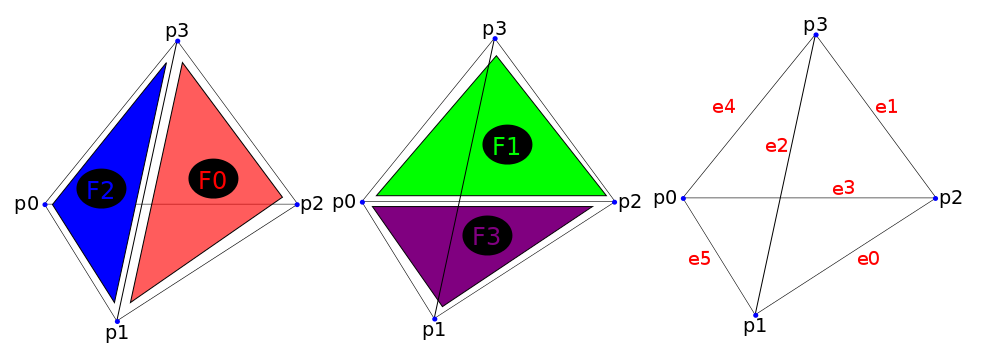
\includegraphics[width=1.0\linewidth]{figures/cutting/tetconfig3.png}
  \caption{\label{fig:tetconfig3}
  {A tetrahedral element in its canonical view. Iterating over nodes, edges and faces of each element is
  one of the primary operations in a geometric algorithm that manipulates such elements. The order we chose here is not the
  only possible one but it simplifies the cutting algorithm and element subdivision process as we will see later.}
}
\end{figure}


In a complex mesh of tetrahedral elements accessing each of these components is a necessary requirement for 
implementing any topological modifications. Therefore the main module in our cutting algorithm is an edge-based
data structure that maps tetrahedral elements to their associated faces and the faces to their associated edges and
finally the edges to their nodes. The minimal set of operations frequently used by most algorithms are as following:

\begin{itemize}
 \item Access to individual vertices, edges, faces and tetrahedral elements. This includes the enumeration of 
 all elements in unspecified order.
 
 \item Per each vertex, access to all the directly adjacent nodes to that vertex (i.e. one ring neighborhood see figure \ref{fig:meshlinks}). 
 A typical use-case for this operation is the uniform distribution of the external forces applied to the mesh. 
 Also many mesh simplification algorithms are based on such operators.
 
 \item Top-down and bottom-up hierarchical access to the mesh entities (An example is shown in figure \ref{fig:meshlinks}). Top-down access 
 is inherently provided in the structure of the mesh entities e.g. elements are comprised of faces and faces are made up of set of edges etc. 
 In case of the bottom up access some algorithms will benefit to have the incident edges of a certain node, or in case of edges all the incident 
 faces of a given edge and for a given face all the incident elements to a particular face in the mesh. This type of access patterns are particularly 
 useful for topological modification scenarios and the required book-keeping operations.
 
 \begin{figure}[H]
  \centering
  % the following command controls the width of the embedded PS file
  % (relative to the width of the current column)
  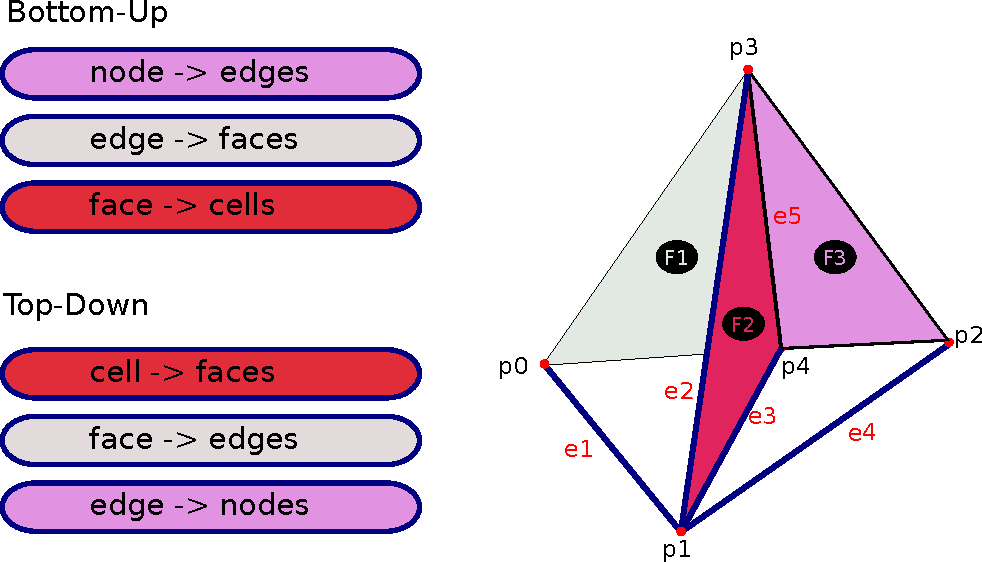
\includegraphics[width=0.8\linewidth]{figures/cutting/mesh_links.pdf}
  \caption{\label{fig:meshlinks}
  {Top-down and bottom-up mesh links. The top-down relationships is explicitly defined in the structure of the mesh.
  An example of the bottom-up links is shown here: Edges $e_1..e_4$ are incident to node $p_1$ and therefore the set 
  $\{p_0$, $p_2$, $p_3$, $p_4\}$} is the one-ring neighborhood of node $p_1$. Faces $F_1..F_3$ are incident to edge 
  $e_5$ and both tetrahedral cells are incident to face $F_2$.
}
\end{figure}

 \item Insertion and removal operations for nodes, edges, faces and elements. These operations require extra care in order to keep
 the top-down and bottom-up links up-to-date. As we will see in our cutting algorithm deferred removal operations can make process much simpler by
 delaying the actual removal until after all the identified entities are visited and the new entities are inserted to the structure.
 This is due to the fact that removal operations will update the internal links between mesh entities therefore two consecutive access operations
 might find the mesh at different states which is not intended in the original proposed algorithm.
 
 \item Update operations for nodes, edges, faces and elements. What is important here is to keep the top-down and bottom-up links up-to-date. 
 For-instance in case of an edge update as soon as the two endpoints of the edge is modified all the incident faces (higher level entity) 
 of that edge and also all the incident edges of the end points of the edge (lower level entity) should be updated.
\end{itemize}

The rest position of each node is stored which can be used to update the physics model and to interpolate the position 
of newly added nodes in case of cutting. Accessing edges using the bottom-up structure is expensive: First the list of incident 
edges to one of the endpoints of the edge is accessed and then a serial search on that list is done to find an edge with the matching 
end points. This has logarithmic complexity with respect to the number of edges in the structure. Instead we chose to use a hash-table
to access edges using a key derived from the two end-points of the edge. Below is how this key is computed for a given edge 
\cite{Mario2010PolygonMesh, Bloomenthal1997}:

\begin{equation}
 key64 = (nodes\left[ 1 \right] << 32) \And nodes\left[ 0 \right]
\end{equation}

This computation is performed when a new edge in inserted into the structure and can produce keys for $2^{64}$ edges uniquely. 
The hash-map then associates this key to its corresponding edge index thereby providing constant-time access. 
Using this technique the faces can also be accessed though their associated node indices which can be convenient for some applications. 

Nothing is removed directly from the mesh storage buffers but rather upon cutting, the elements
are added to the $freelist$ and later the garbage collection removes all the $freelist$ items from the mesh storage buffers. 

When cutting an edge, an edge-update process is performed followed by a new edge insertion. 
The update process splits the original edge in two. Algorithm \ref{alg:edgesplit} describes this process (also see figure \ref{fig:splitedge}):

\begin{algorithm}[H]
\caption{Splitting an edge in our volumetric mesh data structure. The input to this algorithm is the index of the edge to be splitted
and the distance $t$ along the edge where the intersection happens. Figure \ref{fig:splitedge} shows this operation in detail. }
\label{alg:edgesplit}
\begin{algorithmic}[1]	
  \STATE $edge \gets fetchEdge(index)$
  \STATE $n0 \gets fetchNode(edge.from)$
  \STATE $n1 \gets fetchNode(edge.to)$
  \STATE $newp0.rest = n0.rest + (n1.rest - n0.rest) * t$
  \STATE $newp0.pos = n0.pos + (n1.pos - n0.pos) * t$
  \STATE $idxNewP0 \gets addNewPoint(newp0)$
  \STATE $newp1 \gets newp0$
  \STATE $idxNewP1 \gets addNewPoint(newp1)$
  
  \STATE $setEdge(index, edge.from, idxNewP0)$
  \STATE $insertEdge(idxNewP1, edge.to)$

\end{algorithmic}
\end{algorithm}

Algorithm \ref{alg:edgesplit} starts by computing the co-located intersection points $newp0$ and $newp1$ using the provided distance $t$
and the end-points of the original edge. Then both the current and rest positions of the new points are computed. The new points are appended to the 
appropriate mesh storage lists and the current edge is updated to end at $newp0$. Another edge from $newp1$ to the original end point is added later.
Figure \ref{fig:splitedge} shows this process.


\begin{figure}[H]
  \centering
  % the following command controls the width of the embedded PS file
  % (relative to the width of the current column)
  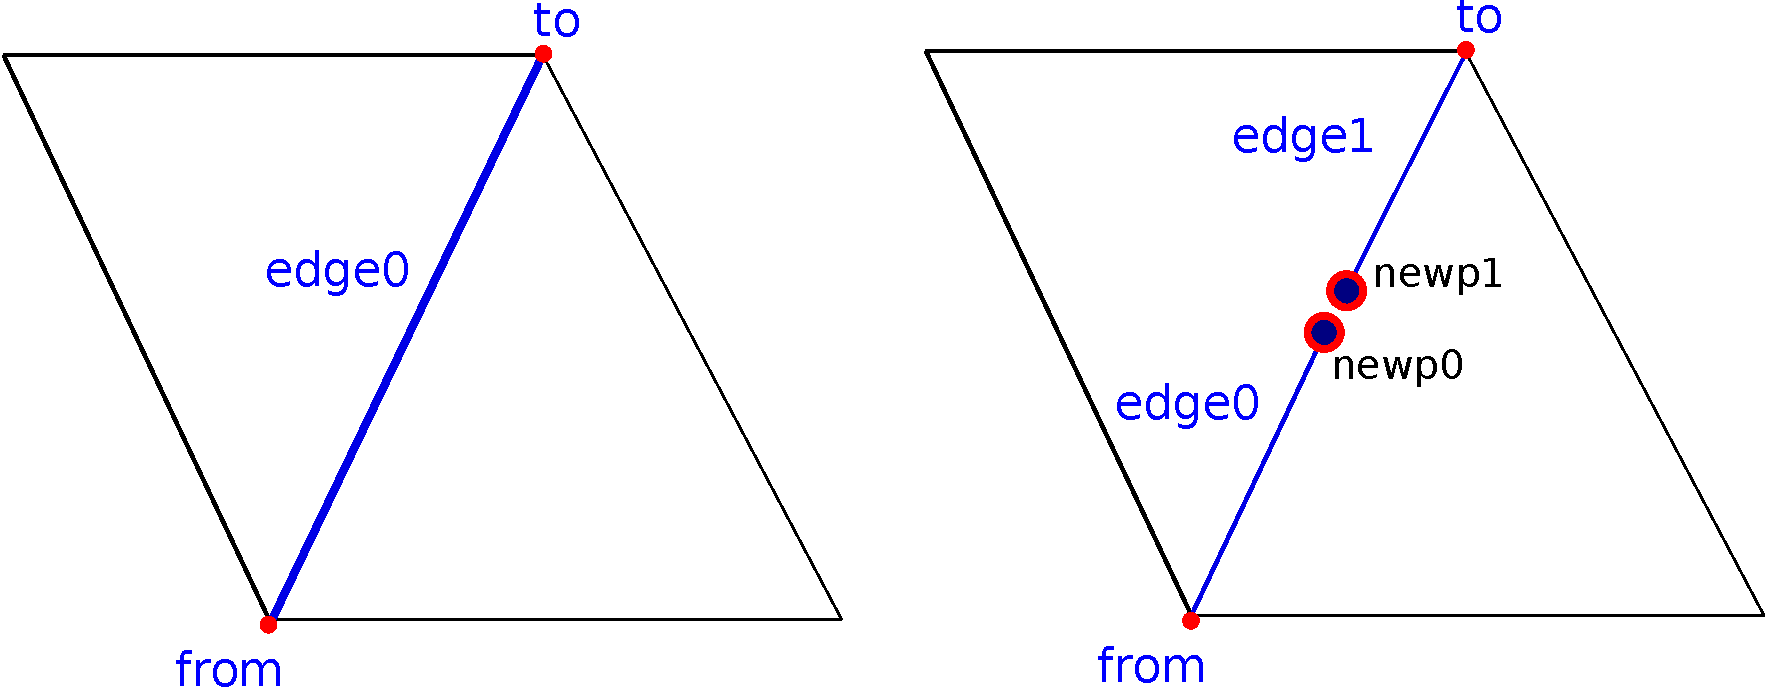
\includegraphics[width=0.8\linewidth]{figures/cutting/splitedge.pdf}
  \caption{\label{fig:splitedge}
  {Left: The edge to be split. Right: Splitting an edge produces a new edge from the point of 
  intersection to the original endpoint. New points $newp_0$ and $newp_1$ are initially co-located.}
}
\end{figure}


Upon topological modifications, events are generated to notify cutting algorithms of the internal changes in the mesh structure. 
This is also useful for debugging and evaluation purposes and can be logged for accounting the sequence of changes made to the 
original mesh. The events include update, insertion and removal of nodes, edges, faces and elements.


In the next section we describe the cutting algorithm which is based on the edge-based data structure presented in this section.

\section{Cutting Algorithm}
\label{sec:cutalg}
Our cutting algorithm follows the same strategy presented by Ganovelli \etal \cite{Ganovelli2000} which suggests use of lookup tables to 
handle different configurations. We also applied the optimizations suggested by
Steinemann and Mor \etal \cite{Steinemann, Mor2000} to have minimal new elements added to the mesh cut. 
The first stage in our cutting algorithm is detecting the cut sweep-surface. The input to this stage is the cut trajectory which is a list of points
that the scalpel passed through in Euclidean space. The cut trajectory is not collected until the axis-aligned bounding box of the cutting tool intersects
with that of the tissue. The tissue bounding box is expanded to rule out the boundary cases where the surface of the model contacts with its own bounding 
box. In such cases the scalpel might miss the surface if the bounding box test fails to detect the initial contact. 


\subsection{Edge Intersections}
\label{sec:CuttingEdgeIntersections}
Using a GPU kernel function the intersection of the sweep-surface and all the edges of the model are computed. 
The input to this stage is the list of edges of the model and 4 points defining the sweep-surface quadrilateral. 
Since the intersection of a triangle and a line segment is faster to compute than a quadrilateral, we 
use two intersection tests per each edge to figure out whether the segment is split or not. The implementation
of our edge triangle intersection follows the Ray-Triangle intersection test given in \cite{RTR3}.


Similar to our GPU polygonization method in section \ref{sec:surfextraction}, a prefix-sum operator counts the number
of intersections and also compacts the resulting array of intersection points. The final output of this stage is a list
of intersection points and the associated edge indices. 
		     
\begin{algorithm}[H]
\caption{\textit{EdgeIntersections} The kernel function that computes intersections of edges 
and the sweep-surface. The prototype of the kernel follows the listing above and the algorithm here represents one 
thread of the execution. }
\label{alg:edgeIntersections}
\begin{algorithmic}[1]	
  \IF{$dim.x \geq countEdges$}
  \STATE return
  \ENDIF
  \STATE $scanFlags[dim.x] \gets 0$
  \STATE $tri0 \gets triangle(0, 1, 2, sweepSurface)$
  \STATE $tri1 \gets triangle(0, 2, 3, sweepSurface)$
  \STATE $edge0 \gets edgeBuffer[dim.x * 2]$
  \STATE $edge1 \gets edgeBuffer[dim.x * 2 + 1]$
  \STATE $res \gets IntersectSegmentTri(edge0, edge1, tri0, p)$
  \IF{$res = 0$}
  \STATE $res = IntersectSegmentTri(edge0, edge1, tri1, p)$
  \ENDIF
  \IF{$res \neq 0$}
  \STATE $scanIntersections[dim.x] \gets p$
  \STATE $scanIndices[dim.x] \gets dim.x$
  \STATE $scanFlags[dim.x] \gets 1$
  \ENDIF
  
\end{algorithmic}
\end{algorithm}

Each thread of execution will examine one edge of the mesh. The blade quadrilateral is divided to two triangles named $tri0$ and $tri1$ 
as shown in algorithm \ref{alg:edgeIntersections}. The two endpoints of the current edge are retrieved from the mesh storage buffer called 
$edgebuffer$. The function named ``IntersectSegmentTri'' computes the intersection point of a line segment and a triangle. If the
first triangle does not intersect with the blade end-points the test is repeated for the second triangle. If there is a
valid intersection point, it is stored in the appropriate output buffer ``scanIntersections'', the index of the intersected edge is stored at
``scanIndices'' and a flag that later identifies successful intersection tests is written to ``scanFlags''. These buffers are compacted later 
using sum-scan operators discussed in the previous chapter. 


\subsection{Produce cut-node list}
\label{sec:CuttingProduceCutNodeList}
Following the improvement made by Steinmann \etal \cite{Steinemann} to minimize the number of subdivided elements; 
per each intersection point which is ``too close'' to one of the edge endpoints; 
the sweep surface is snapped to that endpoint (see figure \ref{fig:cutnode}). The associated endpoint is also stored in a separate list called ``cut-nodes''. 
In our system if an intersection point lies within the 20 percent of its associated edge length radius then it is considered 
as a ``cut node''. This value avoided the most skinny elements. An analysis on the quality factors of the tetrahedral elements 
is made later in this chapter. The cut-nodes are later used to produce special subdivision cases which output non-skinny 
tetrahedral elements.

\begin{figure}[H]
  \centering
  % the following command controls the width of the embedded PS file
  % (relative to the width of the current column)
  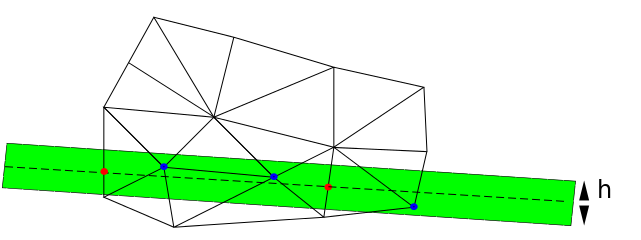
\includegraphics[width=0.8\linewidth]{figures/cutting/cutnode.png}
  \caption{\label{fig:cutnode}
  {Dashed line represents the cut trajectory. For all the edges intersected by the cut sweep surface the end point closest to the sweep surface is selected.
  If the node lies within a threshold h, it is marked as a cut-node painted in blue and all the incident edges to that node are removed from the cut-edges list.
  The red dots are the intersection points associated with the remaining cut-edges.}
}
\end{figure}

\begin{algorithm}[H]
\caption{\textit{ProduceCutNodeList} The function that builds the cut-nodes list from the intersected edges.
If an intersection is within the predefined distance of an edge endpoint it is considered as a ``cut-node''.}
\label{alg:produceCutNodes}
\begin{algorithmic}[1]	
  \FOR{$i = 0$ \TO $cutEdges.count - 1$} 
  \STATE $ce \gets cutEdges\left[i\right]$
  \STATE $edge \gets mesh.edge(ce.handle)$
  \STATE $normalizedT \gets ce.t / length(edge.from, edge.to)$
  \IF{$normalizedT < h$}
  \STATE $cutNodes.insert(edge.from)$
  \ELSE
    \IF{$normalizedT > 1.0 - h$}
    \STATE $cutNodes.insert(edge.to)$
    \ENDIF
  \ENDIF
  \ENDFOR
\end{algorithmic}
\end{algorithm}

In algorithm (\ref{alg:produceCutNodes}) the intersection distance is normalized using the length of the associated edge.
If the normalized distance is within the predefined threshold $h$ then the start point of the edge is a cutnode. Otherwise
if the condition is true on the other end point then that end point is added as the cut-node.

\subsection{Filter intersected-edges}
All the edges that are incident to a ``cut-node'' are removed from the list of intersected-edges. Since our mesh data structure 
already has the bottom-up links, it is trivial to access all the incident edges per each node. 


\subsection{Compute configuration codes for cut elements}
\label{sec:cutconfigs}
After building the list of cut-edges and cut-nodes, all the tetrahedral cells are inspected for intersection. 
The list of cut-edges and cut-nodes are implemented as hash-tables in our system, therefore, performing a query operation can be done 
in constant time and this step is not bottleneck in our system. Per each cell all the 6 edges are checked against the cut-edges hash table 
in the same order given in figure \ref{fig:tetconfig3}. If an edge is included in the cut-edges hash table then a flag bit is set for that
particular edge. The same process is performed for the 4 nodes of each cell and a 4 bits cutnode code is computed for that cell.
Using the lookup table given in table \ref{table:allcutconfigs} and the number of cut-edges and cut-nodes; per each cell a cut configuration
is computed.  If the number of cut-edges and cut-nodes are both zero then that cell is left intact otherwise it is added to the list of intersected cells
to be processed later.

\begin{table}[H]
\begin{center}
\caption{\label{table:allcutconfigs}{The following look-up table is used to differentiate between different cutting configurations based on
the number of cut-edges and cut-nodes. All cases subdivide tetrahedral elements into smaller cells except for case Z where the original
cell is left intact.}}
  \begin{tabular}{ | l | c | c | c | }
    \hline    
    type & state & \#cut edges & \#cut nodes \\ \hline \hline    
    A & complete & 3 & 0 \\ \hline
    B & complete & 4 & 0 \\ \hline
    C & progressive & 1 & 0 \\ \hline
    D & progressive & 2 & 0 \\ \hline
    E & progressive & 3 & 0 \\ \hline
    X & complete & 2 & 1 \\ \hline
    Y & complete & 1 & 2 \\ \hline
    Z & complete & 0 & 3 \\ \hline
    \hline
  \end{tabular}
\end{center}
\end{table}

Based on its cut configuration a tetrahedral cell is subdivided into smaller elements. In our system a separate lookup table is 
implemented per each of the above cut configurations. The reason is that each configuration leads to a different number of subdivided elements, however;
it is also possible to combine all lookup tables into one. Table \ref{table:lutcutA} shows the generated cells for the cut type A.
In this configuration only 3 out 6 edges of a tetrahedra are cut and that should lead to $C(n, r) = C(6, 3) = 20$ different cut edges (without repetition and
order does not matter). However, valid cut edges are the ones that separate one node from the other three that will lead to the compact lookup table in \ref{table:lutcutA}.
The first column is the cut-edge code associated with that configuration row e.g. A56 denotes cut type A with edges 3, 4, 5 being cut where each each represent one bit in 
the code. The second column is the list of generated tetrahedral cells. Cut A produces 4 cells. Nodes 0-3 are the original nodes creating the original cell. When each edge 
shown in figure \ref{fig:tetconfig3} is cut in the middle two additional nodes are added to that cell these extra nodes are defined at indices 4-15 as shown in figure 
\ref{fig:midpoints}.

The lookup table for type B is shown in table \ref{table:lutcutB}. Four edges are being cut in configuration type B and per each cell 6 sub-elements are generated.
Cutting 4 out of 6 edges should result in $C(n, r) = C(6, 4) = 15$ distinct cut-edges. However, using the same analogy only 3 valid cuts are able to split the cell 
in two disjoint parts. Those cuts are summarized in table \ref{table:lutcutB}. 

Case Z is trivial since the cell is left intact. For case Y two tetrahedral elements are being generated and one edge is being split only. Case X is very similar to
A in the sense that one original node is being separated from the rest of the simplex. In cases X and Y the cut-nodes are duplicated and the new cells are generated based
on the split edges and the original nodes and their associated duplicates. Since we haven't implemented progressive cutting yet cases C, D and E are left for future work.

\begin{table}[H]
\begin{center}
\caption{\label{table:lutcutA}{Lookup table for generating sub-elements for type A configuration}}
  \begin{tabular}{ | l | c | c | }
    \hline    
    config & cut edges & generated cells \\ \hline \hline    
    A56 & 3, 4, 5 & \{0, 12, 10, 14\}, \{3, 13, 11, 15\}, \{3, 1, 15, 11\}, \{1, 2, 3, 11\} \\ \hline
    A37 & 0, 2, 5 & \{1, 4, 8, 15\}, \{3, 9, 5, 14\}, \{0, 3, 14, 5\}, \{0, 2, 3, 5\} \\ \hline
    A11 & 0, 1, 3 & \{2, 5, 6, 11\}, \{3, 7, 10, 4\}, \{3, 1, 4, 10\}, \{0, 1, 3, 10\} \\ \hline
    A22 & 1, 2, 4 & \{3, 13, 9, 7\}, \{1, 8, 12, 6\}, \{1, 2, 12, 6\}, \{0, 1, 2, 12\} \\ \hline
    \hline
  \end{tabular}
\end{center}
\end{table}

\begin{table}[H]
\begin{center}
\caption{\label{table:lutcutB}{Lookup table for generating sub-elements for type B configuration. 
Sub-elements are separated by semi-colon to fit on the line.}}
  \begin{tabular}{ | l | c | c | }
    \hline    
    config & cut edges & generated cells \\ \hline \hline    
    B46 & 1, 2, 3, 5 & \{2, 6, 11, 1; 8, 11, 15, 1; 6, 11, 8, 1; 3, 7, 9, 10; 3, 10, 0, 9; 0, 14, 10, 9\} \\ \hline
    B51 & 0, 1, 4, 5 & \{3, 7, 13, 15; 15, 1, 4, 7; 15, 1, 3, 7; 0, 12, 14, 6; 2, 5, 6, 14; 0, 14, 6, 2\} \\ \hline
    B29 & 0, 2, 3, 4 & \{4, 10, 12, 0; 0, 8, 12, 4; 0, 8, 1, 4; 3, 9, 13, 5; 2, 5, 11, 3; 3, 13, 5, 11\} \\ \hline
    \hline
  \end{tabular}
\end{center}
\end{table}



\begin{figure}[H]
  \centering
  % the following command controls the width of the embedded PS file
  % (relative to the width of the current column)
  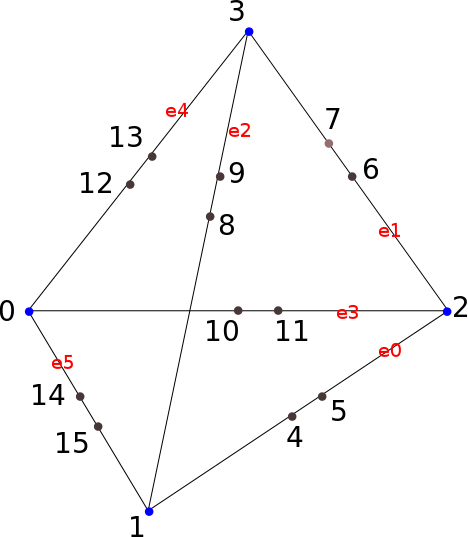
\includegraphics[width=0.4\linewidth]{figures/cutting/midpoints.png}
  \caption{\label{fig:midpoints}
  {Nodes 0-3 are the original cell nodes shown in blue dots. Splitting each of the 6 edges can produce two additional nodes up to 12 more nodes which 
  are placed at indices 4-15 shown in black dots.}
}
\end{figure}
%The main contribution of our cutting method is the GPU-accelerations applied to the cutting process to support interactive topological 
%modifications and the post processing step that supports smoothness of the cuts in case of complex tissues. 

\subsection{Topological Updates}
During the cutting process, the intersected cells are being replaced by sub-cells as discussed in the previous section. Cell removal operation involves updating the entire 
mesh structure which can be expensive if performed during the cut process. In our system all the intersected cells are being placed on a pending list for later deletion 
which will be visited by a post-processing stage called ``garbage collection''. This way the indices of the mesh entities are left intact during the cutting process and 
then once the cut is finalized the mesh can be cleaned and any unused entities such as cells, faces, edges or nodes are being purged to keep the structure as compact as 
possible for the next cutting operations.

\section{Cutting Results}
\label{sec:cutres}
In this section we review the results for the cutting algorithm presented in this chapter. 
Two models are considered for this analysis and a more complex cutting scenario is presented in chapter \ref{chapter:evaluation}.
The model shown in figure \ref{fig:dumbelsexample} is composed of two implicit spheres that are blended and tetrahedralized for 
physics simulation. The resulting volumetric mesh is cut horizontally, vertically and diagonally using the scalpel tool. 

\begin{figure}[H]
  \centering
  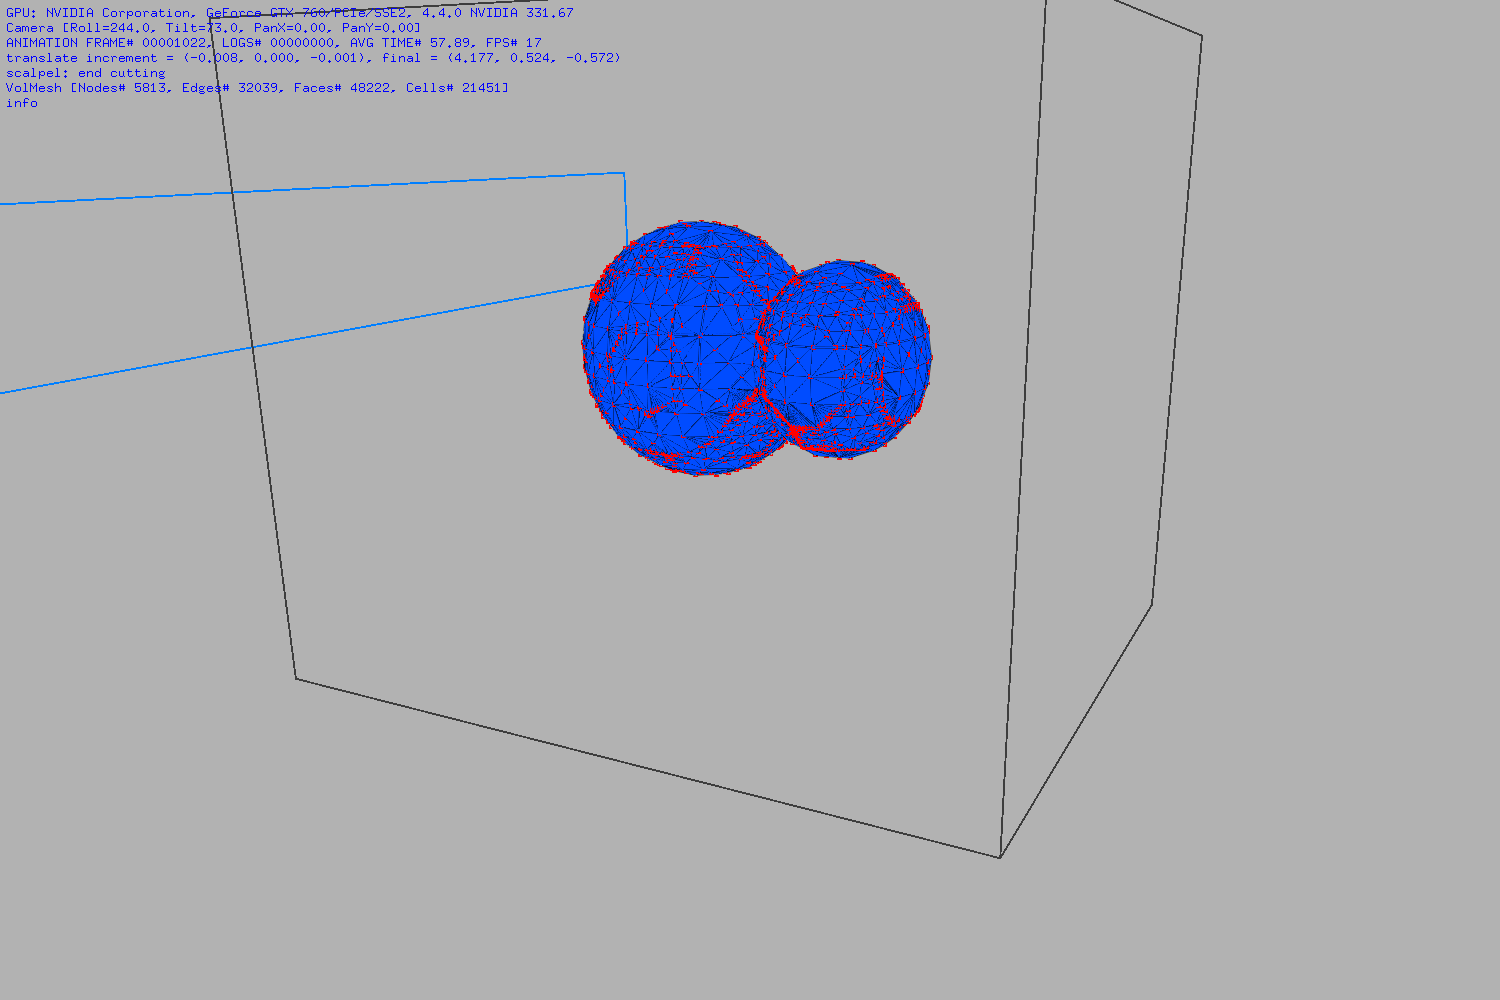
\includegraphics[width=0.4\linewidth]{figures/cutting/dumbel01.png}
  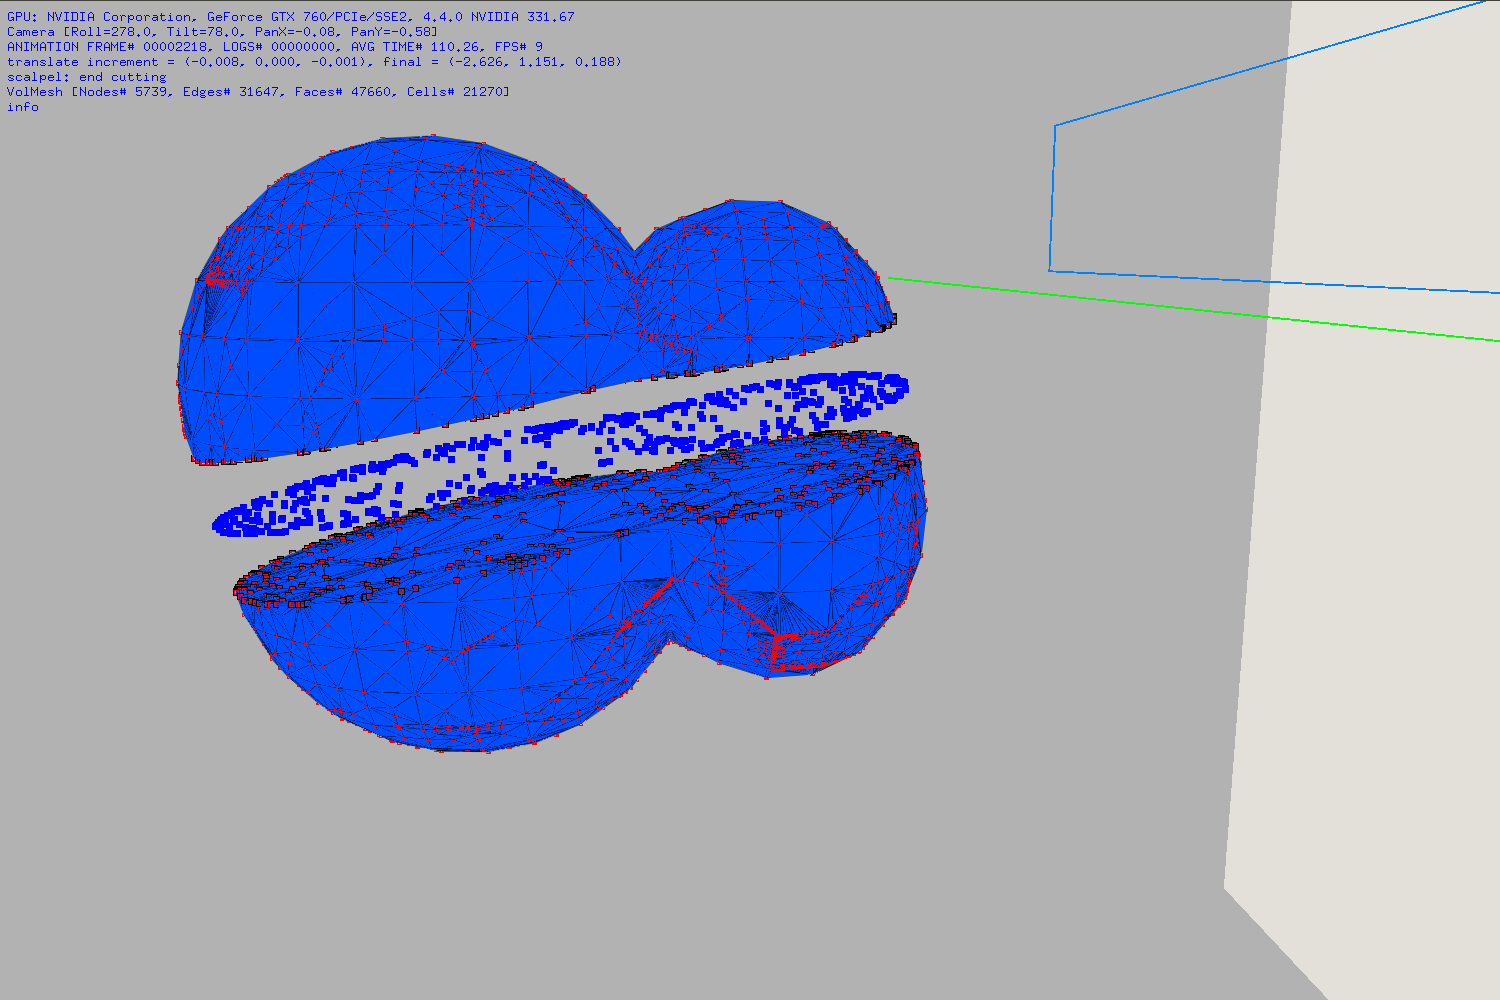
\includegraphics[width=0.4\linewidth]{figures/cutting/dumbel02.png}
  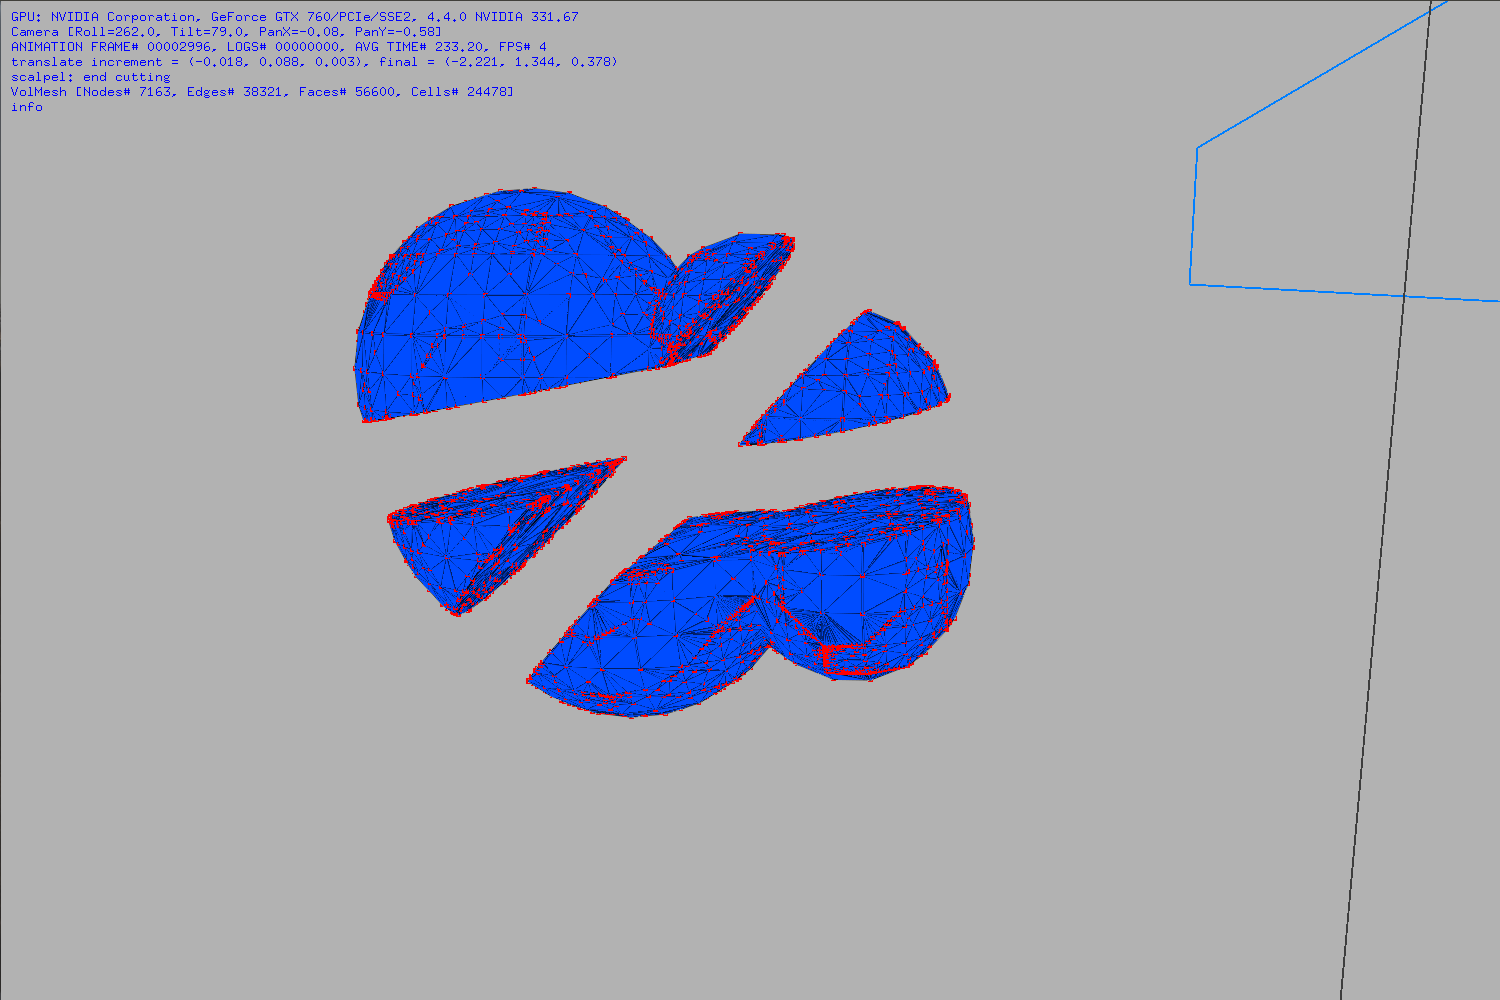
\includegraphics[width=0.4\linewidth]{figures/cutting/dumbel03.png}
  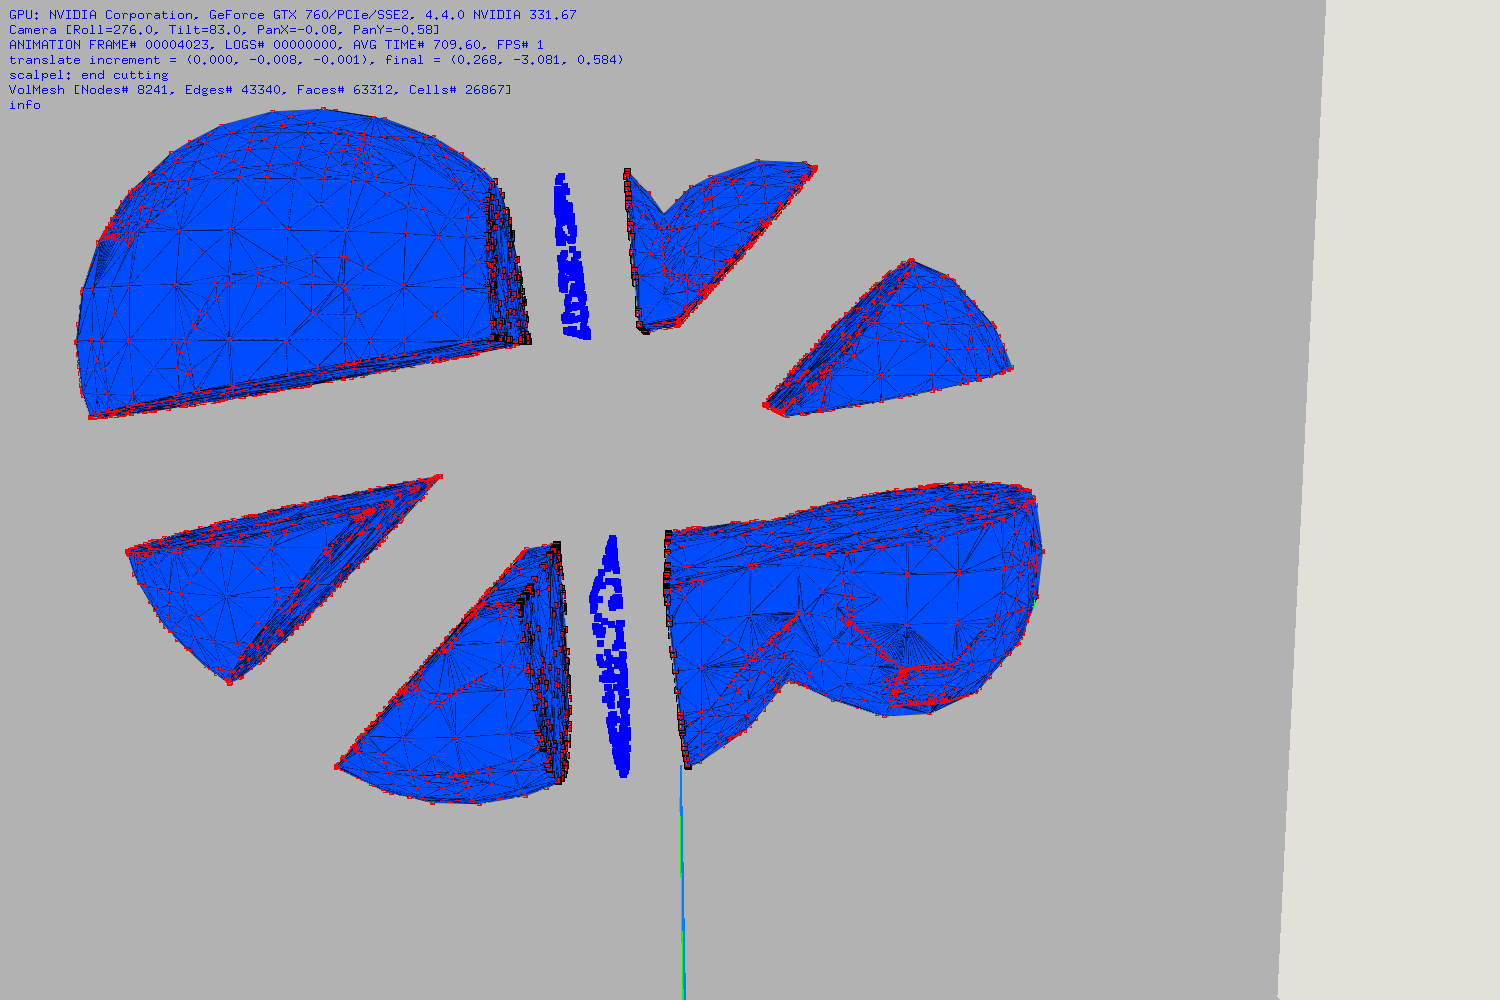
\includegraphics[width=0.4\linewidth]{figures/cutting/dumbel04.png}
  
  \caption{\label{fig:dumbelsexample}
  {Two implicit spheres are blended and tetrahedralized for our physics simulation system. The peanut model is cut 3 times.
  Top-Left: The original volumetric mesh. Top-Right: Model cut horizontally with the scalpel tool.
  Bottom-Left: Diagonal cutting, Bottom-Right: Vertical cut. Blue dot represent the intersection points on the original edges.}
}
\end{figure}

The second model is the tumor model composed of 10 blended spheres. Using the same process the model is tetrahedralized for physical simulation
and cut 3 times. Figure \ref{fig:tumor} shows the result of these topological modifications.


\begin{figure}[H]
  \centering
  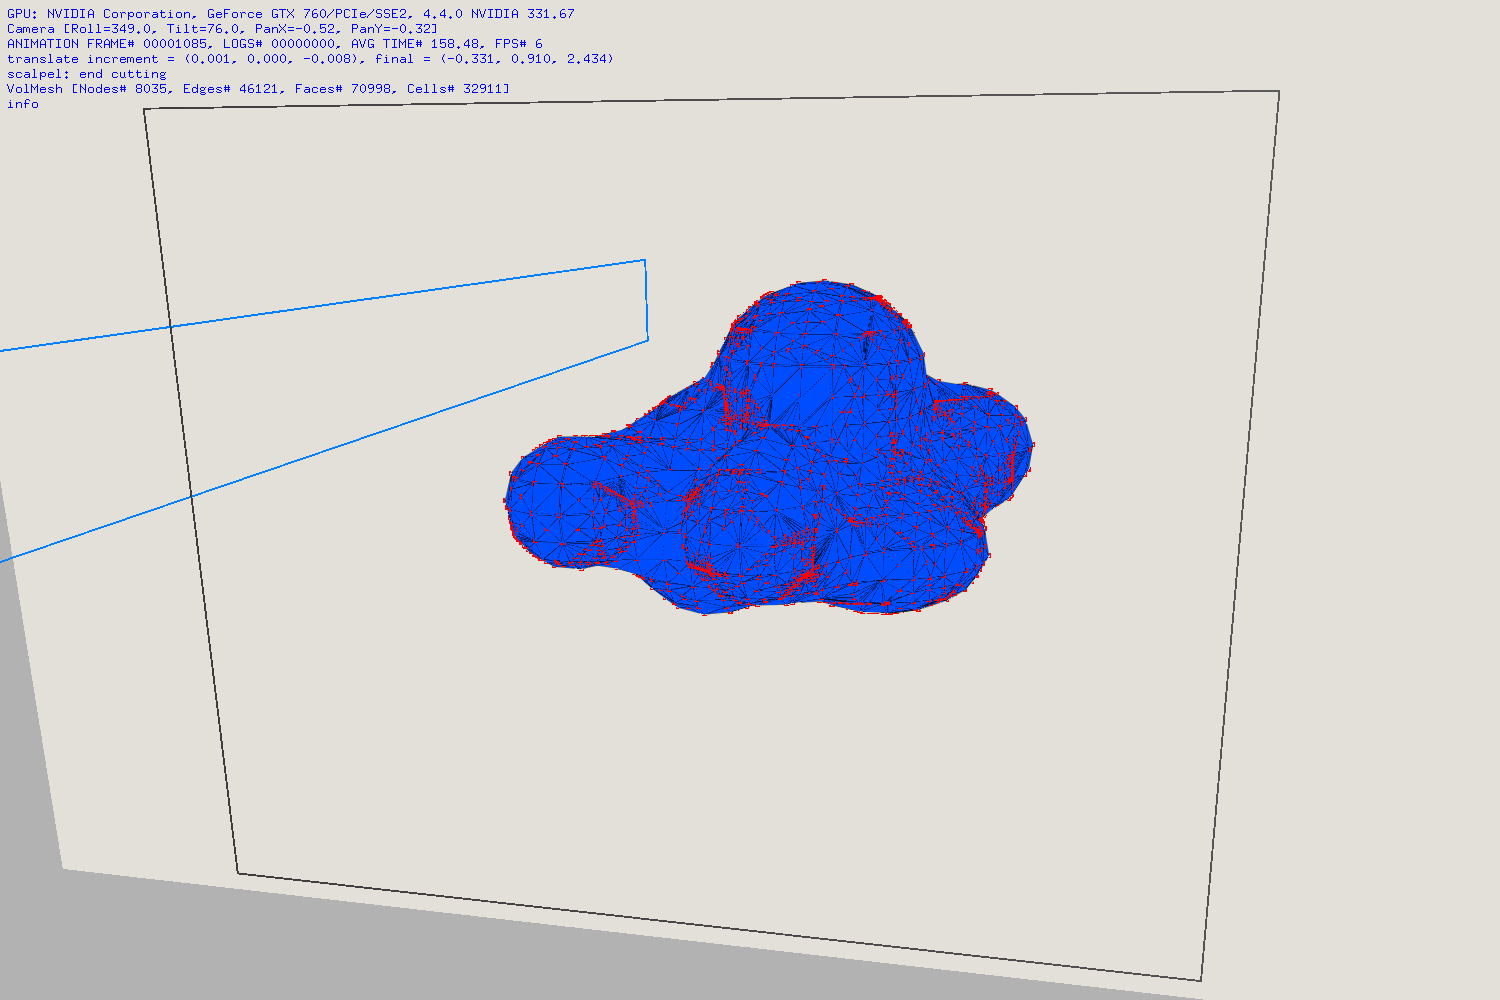
\includegraphics[width=0.4\linewidth]{figures/cutting/tumor01.png}
  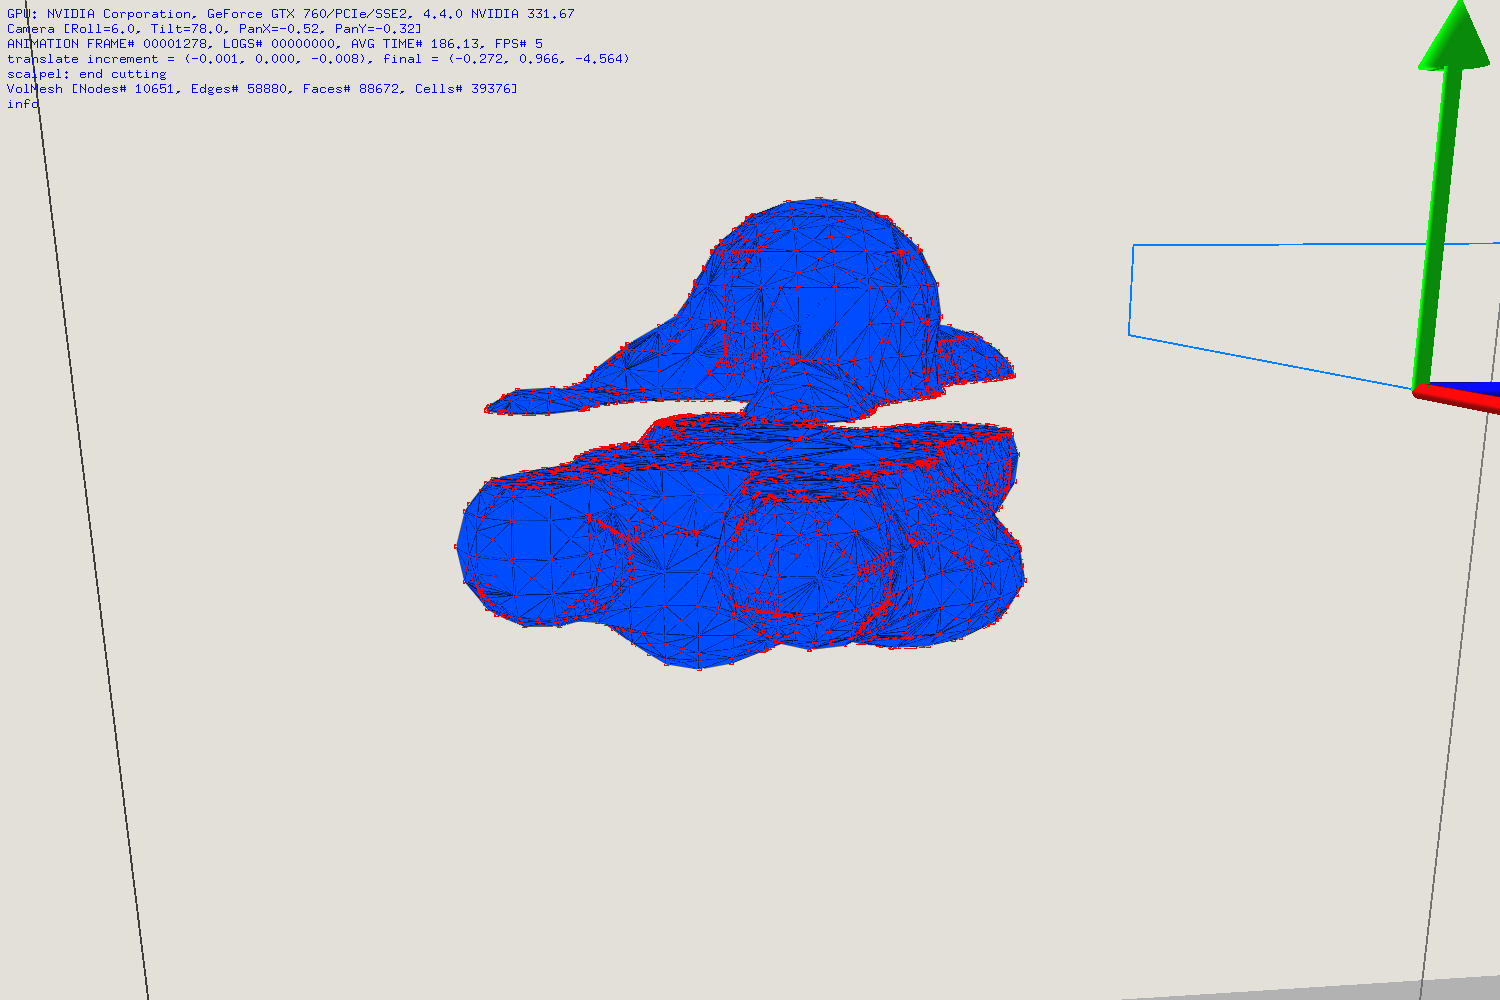
\includegraphics[width=0.4\linewidth]{figures/cutting/tumor02.png}
  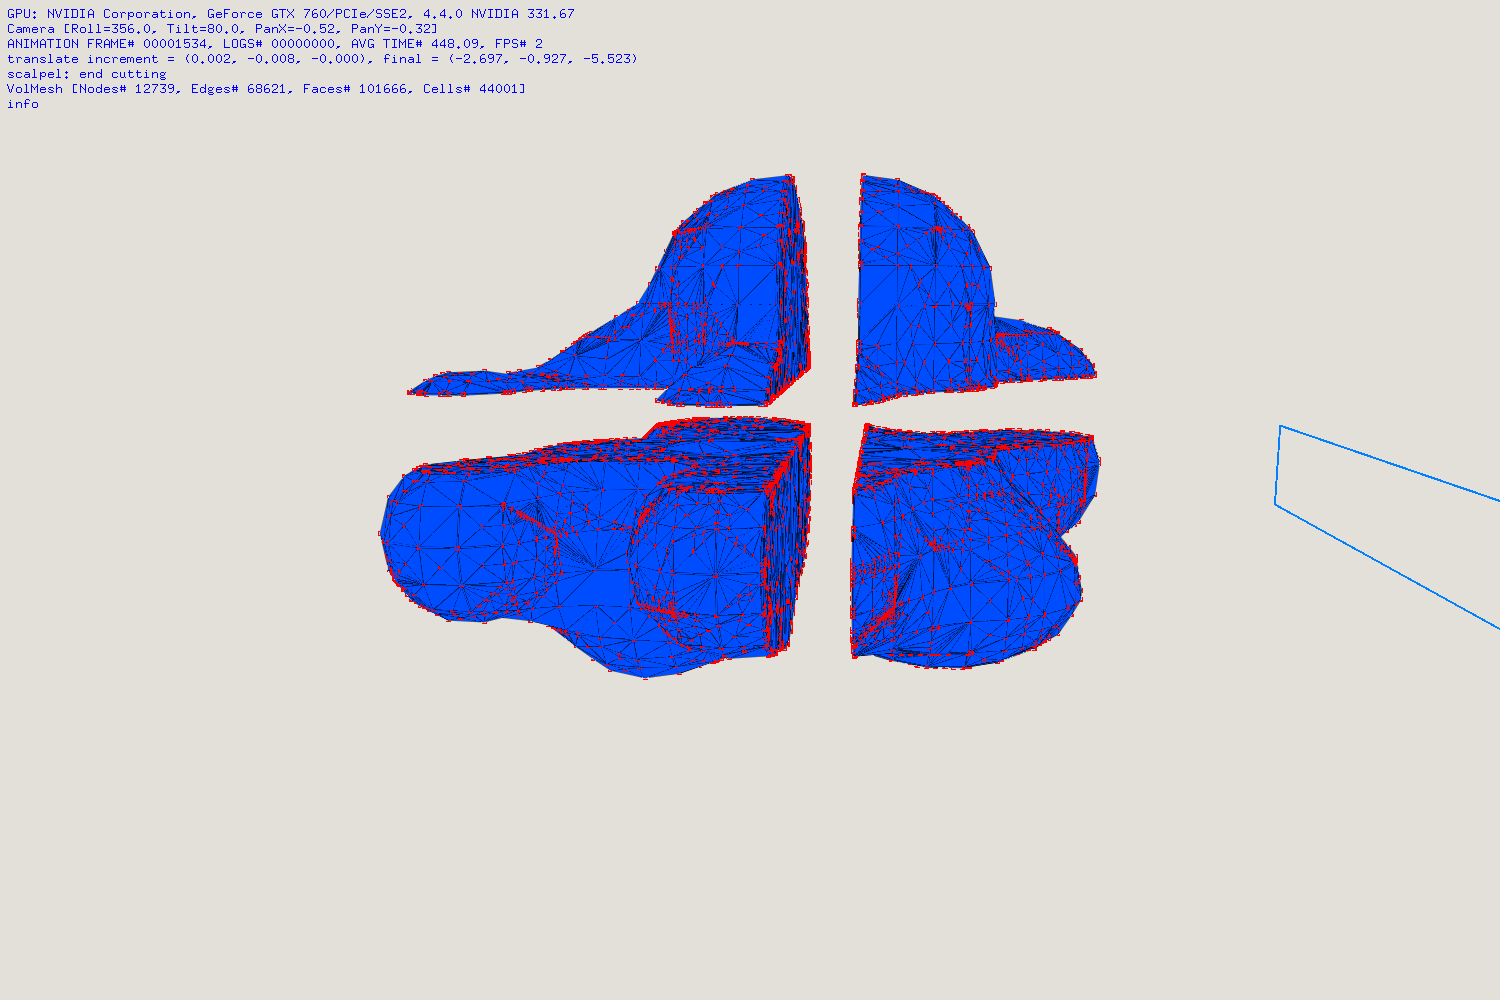
\includegraphics[width=0.4\linewidth]{figures/cutting/tumor03.png}
  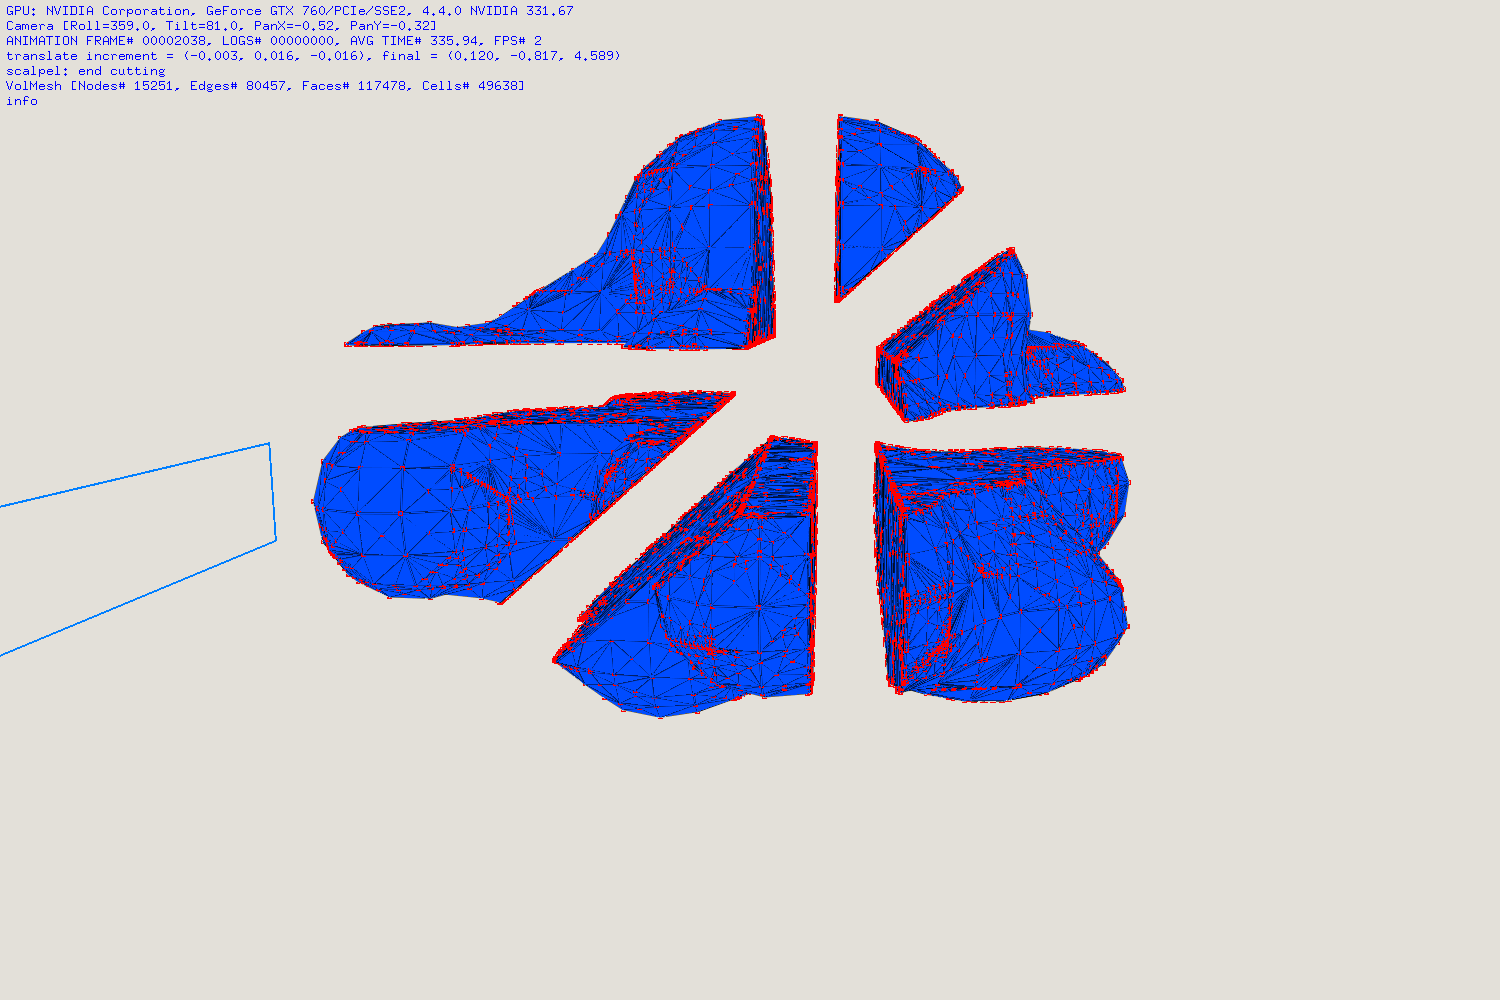
\includegraphics[width=0.4\linewidth]{figures/cutting/tumor04.png}
  
  \caption{\label{fig:tumor}
  {The tumor model above is composed of 10 point primitives and a blending operator. Top-Left: the original mesh, Top-Right:
  The mesh after a horizontal cut, Bottom-Left: The vertical cut, Bottom-Right: mesh after a diagonal cut.}
}
\end{figure}

To analyse the quality of the tetrahedral mesh after the cutting process several attributes are being considered. First, the 
number of elements before and after each cut. More elements will increase the system solve time and degrade the performance of the 
physical simulation due to the larger matrix dimensions involved in the process. Badly shaped (skinny) tetrahedral elements impose stricter constraints 
on the simulation time step \cite{Steinemann, Ganovelli2000}. In order to get an understanding of the quality of the tetrahedral mesh after the cuts, element
counts and several other quality measures are considered \cite{parthasarathy1994comparison}. 

\begin{itemize}
 \item The ratio between largest and smallest tetrahedron volume
 \item The ratio between largest and smallest edge length
 \item The lowest aspect ratio of all tetrahedra 
\end{itemize}

The aspect ratio of a tetrahedra is measured as following:

\begin{equation}
\beta = \frac{CR}{3*IR} 
\end{equation}

Where $CR$ is the circumsphere radius of an element and $IR$ is the inscribed-sphere computed by the following equation 
\cite{parthasarathy1994comparison}:

\begin{equation}
IR = \frac{4V}{\sum_{i=1}^{4} SA_i}
\end{equation}

Where $V$ is the volume of a tetrahedra, $SA_i$ is the surface area of the $i$th triangle face of an element.
 
\begin{table}[H]
\begin{center}
\caption{\label{table:meshquality}{Mesh quality measurements.}}
  \begin{tabular}{ | l | c | c || c | c |}
    \hline    
     & original peanut & peanut after 3 cuts & original tumor & tumor after 3 cuts \\ \hline \hline    
    Nodes & 4437 & 8933 & 8035 & 15821  \\ \hline
    Edges & 25420 & 46466 & 46121 & 82711 \\ \hline
    Faces & 39108 & 67388 & 70998 & 120212 \\ \hline
    Cells & 18124 & 28322 & 32911 & 50605 \\ \hline
    $V_{max} / V_{min}$ & 84.927 & 58.253 & 316.898 & 287.596 \\ \hline
    $l_{max} / l_{min}$ & 42.367 & 47.547 & 40.045 & 130.556 \\ \hline
    $AspectRatio_{min}$ & $3 \times 10^{-7}$ & $3 \times 10^{-7}$ & $10^{-6}$ & $10^{-6}$ \\ \hline
    \hline
  \end{tabular}
\end{center}
\end{table}

Graichen \etal presented an excellent study on the tetrahedral mesh quality measures \cite{Graichen1993}. 
Thin, wedge-like, flat and sliver elements (where 4 points of the element are co-planar) are the source of poor simulation 
results. Table \ref{table:meshquality} summarizes the statistical quality factors before and after cutting the two example meshes. 
The original volumetric mesh of both of these models are extracted from their associated \blob representation using our GPU tetrahedralization
algorithm presented in chapter \ref{chapter:GPUDiscretization}.

As it can be seen from the results the cutting method presented in this chapter does not increase the ratio of maximum to minimum 
volume after the cuts are made. This means that the element subdivision stage in our system does not 
introduce ill-shaped elements to the mesh. The ratio of the maximum to minimum edge-length did not change drastically.
However, a local re-meshing process after the cut specially in the vicinity of the cut region can improve the quality 
of the mesh significantly. 

The element count has increased steadily after each cut operation. Figure \ref{fig:cutting_cells_increase} shows the trend of element increase 
after $N$ cuts are made to the mesh.

\begin{figure}[H]
  \centering
  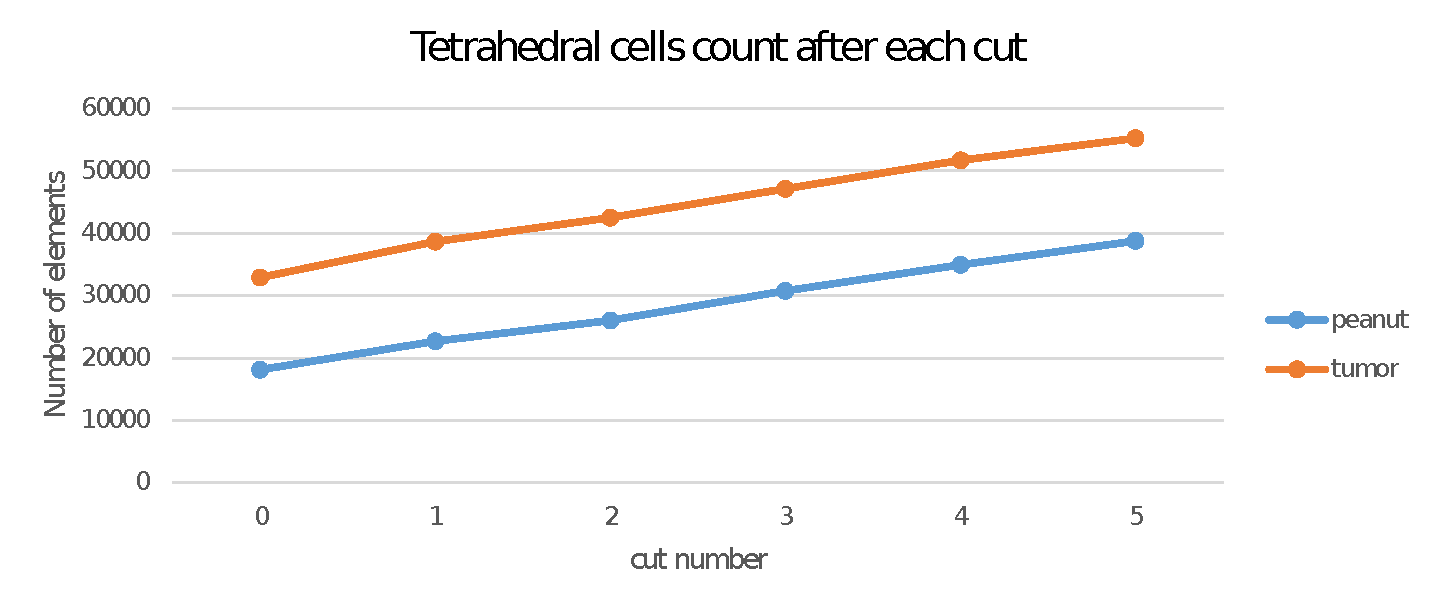
\includegraphics[width=1.0\linewidth]{figures/cutting/cutting_cells_increase.pdf}
  \caption{\label{fig:cutting_cells_increase}
  {Number of tetrahedral cells after each cut operation. The horizontal axis is the cut number starting from cut 0 or the original mesh. 
  The vertical axis is the number of cells.}
}
\end{figure}

Figure \ref{fig:cutting_intersected_vs_new} provides a clear understanding of how many new cells are added to the mesh after each cut operation.
The blue bar in this figure shows the number of cells that are intersected with the cut surface per each cut. Following the algorithm given in 
section \ref{sec:cutconfigs} the intersected cells are subdivided and replaced by new set of generated cells shown in orange. 
On average the ratio of newly generated cells to intersected cells is 3.6 from these results. This is due to the fact that most of the cut configurations
are of type A which result in a 1 to 4 subdivision. 

\begin{figure}[H]
  \centering
  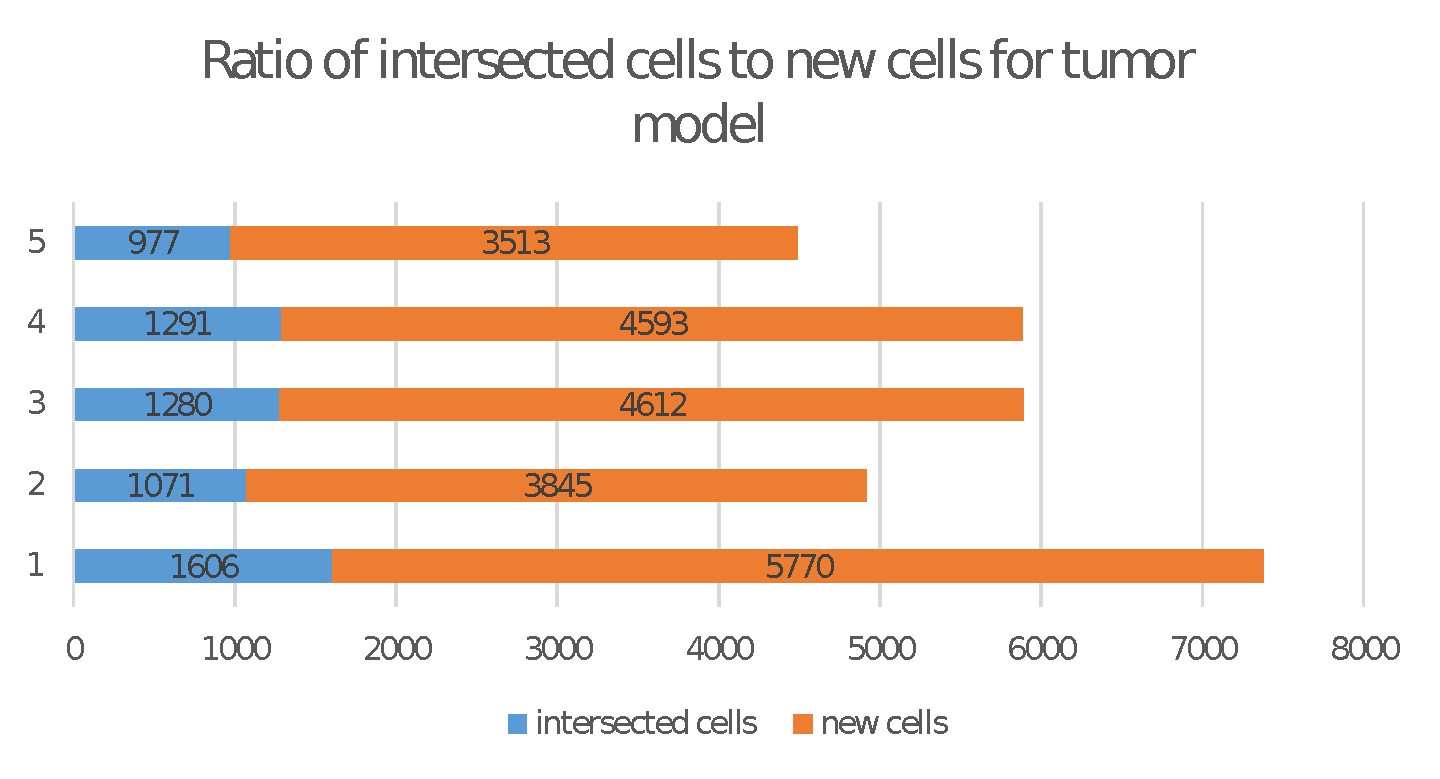
\includegraphics[width=1.0\linewidth]{figures/cutting/cutting_intersected_vs_new_tumor.pdf}
  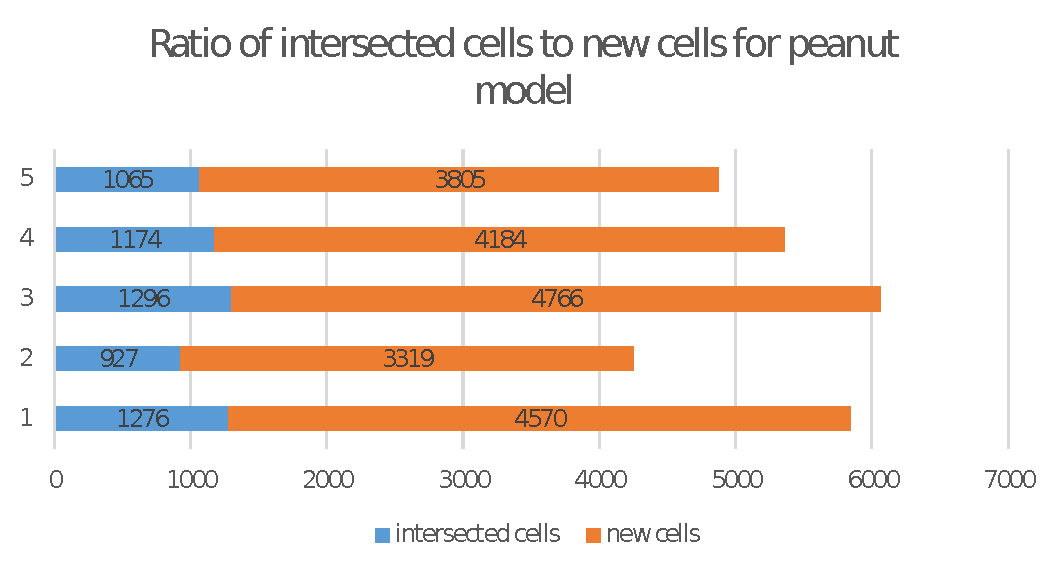
\includegraphics[width=1.0\linewidth]{figures/cutting/cutting_intersected_vs_new_peanut.pdf}
  \caption{\label{fig:cutting_intersected_vs_new}
  {The ratio of intersected cells to newly added cells for tumor (top) and peanut model (bottom). Each blue bar represents the count of cells 
  intersected with the scalpel tool while the orange bar next to it, is the number of newly generated cells after subdividing those intersected cells.}
}
\end{figure}


	\startchapter{Evaluation, Analysis and Comparisons}
\label{chapter:evaluation}
During the past decade a new thrust has appeared with the development of deformable tissue modelling techniques which could make it
possible to develop patient-specific simulations. Whenever the best surgical strategy is unclear or the patient presents a rare
pathology such simulations could be beneficial. Other use-cases for such systems is in surgical skill training which is a long 
and tedious process of acquiring fine motor skills. In all those scenarios physically-based animation of soft tissues is challenging and 
has lots of room for improvement. 

Our methods presented in the previous chapters have been integrated into our surgical simulation system. 
The result is a comprehensive environment for soft-tissue modelling and simulation with support for cutting and
probing. We present our results in the context of a skull craniotomy procedure.

Craniotomy is a surgical operation in which a bone flap is temporarily removed 
from the skull to access the brain. Craniotomies are often a critical operation performed on patients suffering 
from brain lesions or traumatic brain injury (TBI), and can also allow doctors to surgically implant deep brain 
stimulator for the treatment of Parkinson's disease, epilepsy and cerebellar tremor. The procedure is also widely 
used in neuroscience for extracellular recording, brain imaging, and for neurological manipulations such as electrical 
stimulation and chemical titration. Craniotomies are also named according to their size and complexity. Small dime-sized 
craniotomies are called burr holes or keyhole craniotomies. Sometimes stereotactic frames, image-guided computer systems, 
or endoscopes are used to precisely direct instruments through these small holes. Burr holes or keyhole craniotomies are 
used for minimally invasive procedures to:

\begin{itemize}
 \item insert a shunt into the ventricles to drain cerebrospinal fluid (hydrocephalus)
 \item insert a deep brain stimulator to treat Parkinson Disease
 \item insert an intracranial pressure (ICP) monitor
 \item remove a small sample of abnormal tissue (needle biopsy)
 \item drain a blood clot (stereotactic hematoma aspiration)
 \item insert an endoscope to remove small tumors and clip aneurysms
\end{itemize}

In the following sections we review the related work in this domain and then describe our simulation 
setup. The chapter concludes with results and analysis.
%The second simulation operation is brain biopsy which is the removal of a small piece of brain tissue for the diagnosis of abnormalities 
%of the brain. It is used to diagnose Alzheimer's disease, tumors, infection, inflammation, and other brain disorders. By examining 
%the tissue sample under a microscope, the biopsy sample provides doctors with the information necessary to guide diagnosis and treatment.

\section{Architectural constraints}
We are able to perform interactive cuts on a model with more than 60,000 cells. The GPU accelerated cutting algorithm 
presented in chapter \ref{chapter:Cutting} requires a modern GPU with OpenCL support. The system we used for this
experiment is equipped with an Nvidia Geforce GTX760 with 2GB of video memory and 1152 CUDA cores. The CPU is an 
Intel Core i7-4770K with 256 KB, 1MB and 8MB of L1 to L3 cache. This processor has 4 cores and up to 8 threads can run in parallel. 
Our system is also equipped with 16 GB of main memory. 

\section{Eggshell experiment}
Before drilling an actual skull mesh with many tetrahedral elements we tested our system on a spherial model similar to 
an eggshell. This model is composed of 840 nodes and 2280 tetrahedral cells. The outer surface is composed of two layers 
of tetrahedral elements only (see figure \ref{fig:eggshell01}). To create this model implicitly a smaller sphere is subtracted 
from a larger one. After tetrahedralization the mesh is post processed for smoothness.

\begin{figure}[H]
  \centering
  % the following command controls the width of the embedded PS file
  % (relative to the width of the current column)
  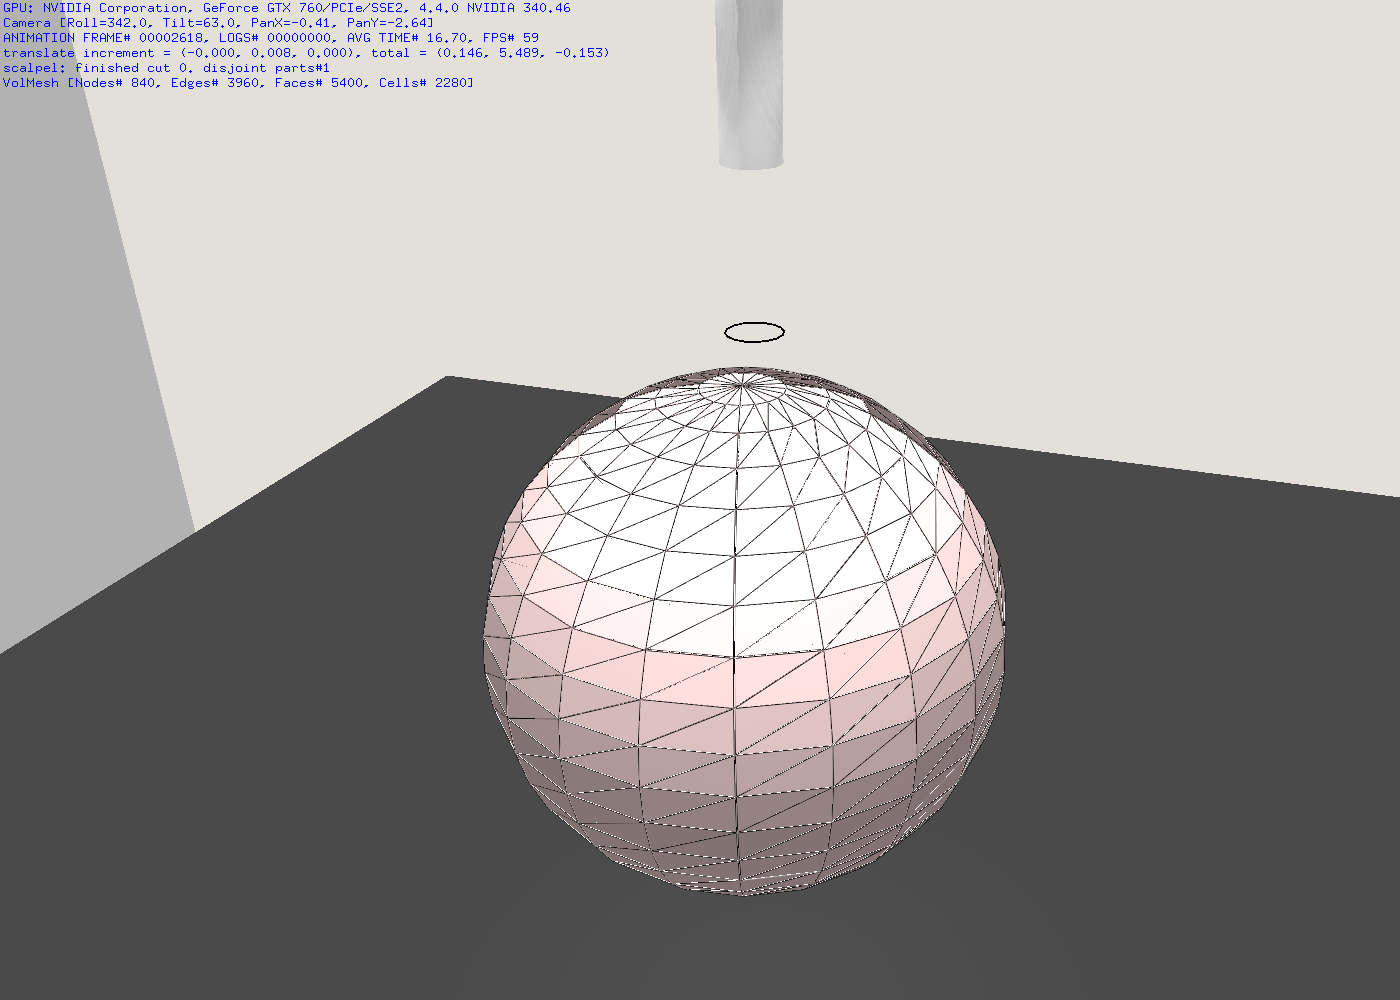
\includegraphics[width=0.7\linewidth]{figures/evaluation/eggshell01.png}
  \caption{\label{fig:eggshell01}
  {Eggshell model before being drilled by our cutting tool.}
}
\end{figure}

After the drilling operation, only 120 new elements are added to the mesh for a total of 2400 elements. The entire process is completed 
interactively. The small disjoint parts fall down on the ground due to gravity. Each disjoint part becomes an independent
deformable model in our system and subject to forces and deformations. Figure \ref{fig:eggshell02} shows the mesh after being 
drilled for the bare hole.


\begin{figure}[H]
  \centering
  % the following command controls the width of the embedded PS file
  % (relative to the width of the current column)
  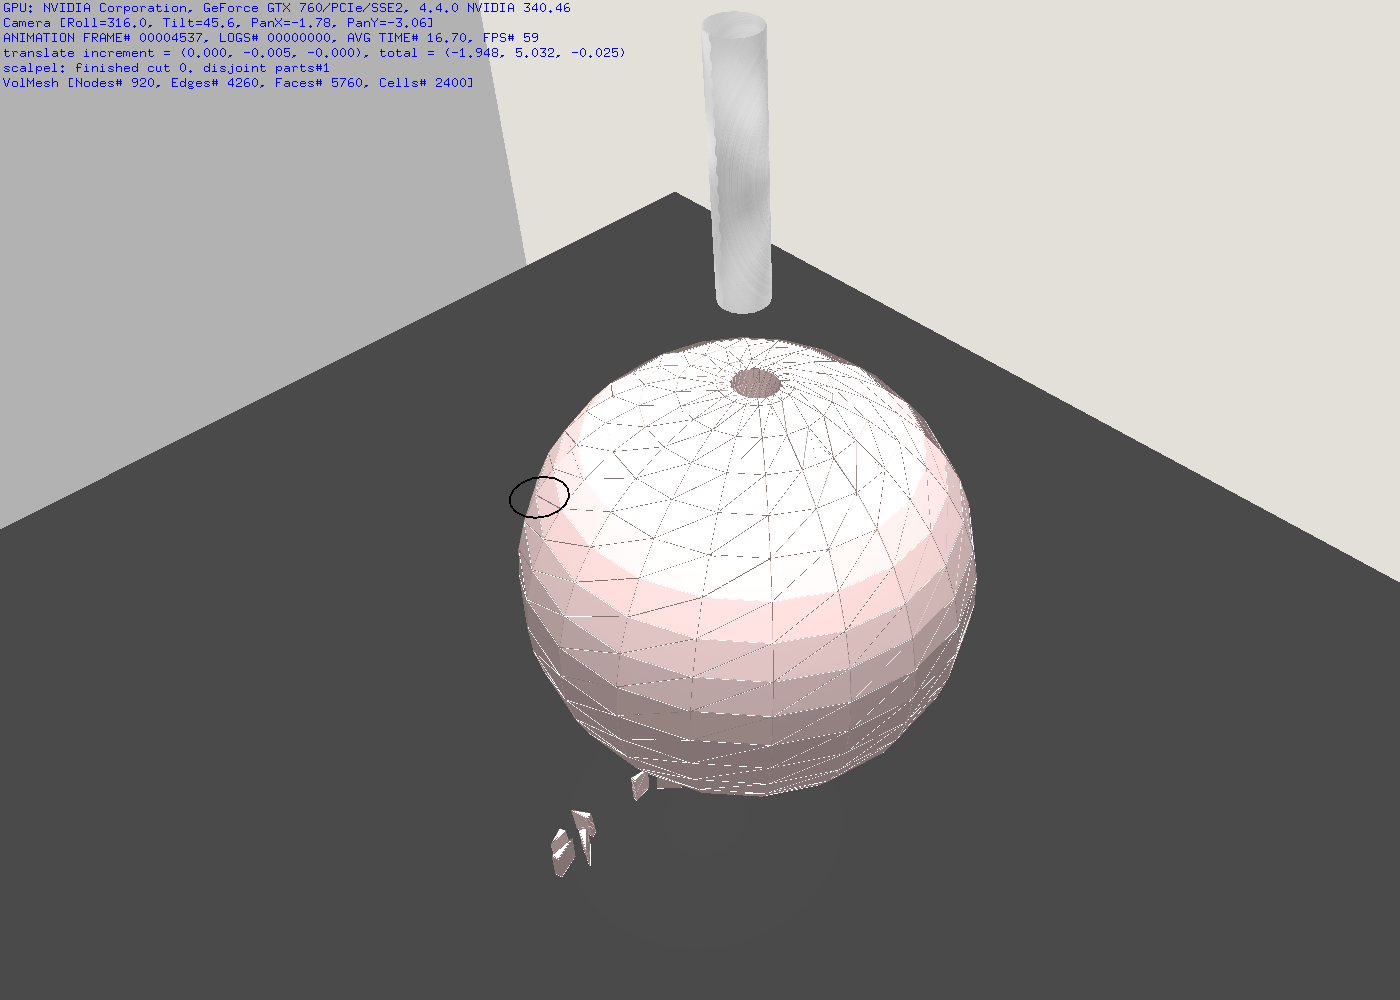
\includegraphics[width=0.6\linewidth]{figures/evaluation/eggshell02.png}
  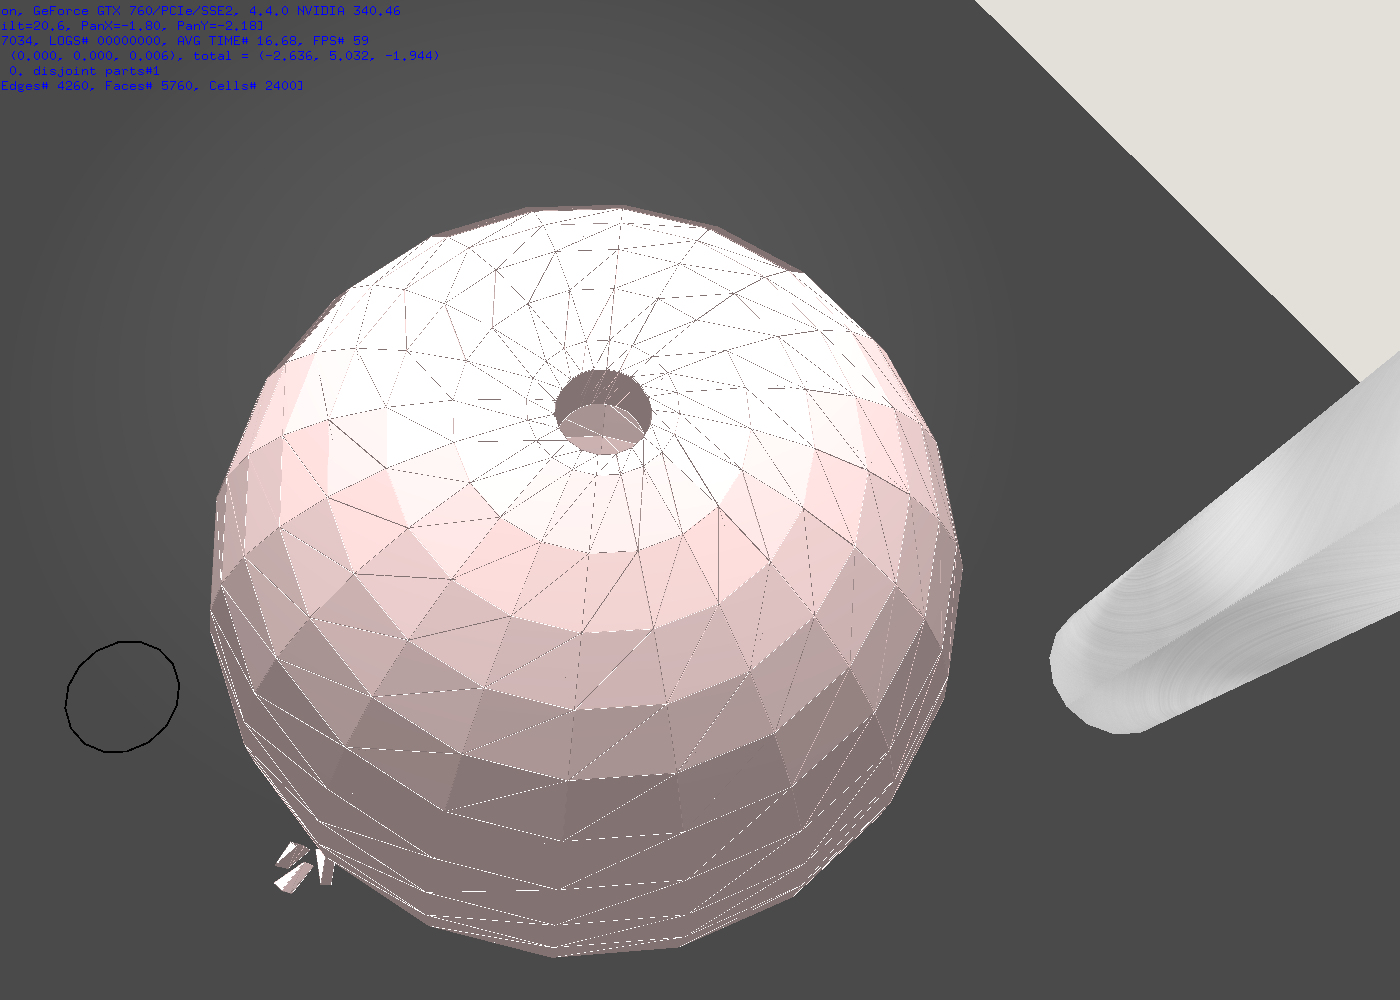
\includegraphics[width=0.6\linewidth]{figures/evaluation/eggshell03.png}
  \caption{\label{fig:eggshell02}
  {Eggshell model after being drilled by our cutting tool.}
}
\end{figure}

After completing this experiment successfully our algorithm showed to be robust enough to handle 
more complex meshes. In the next stage a real data-set of an skull tissue is used for the craniotomy operation.

\section{Craniotomy}
\label{sec:craniotomy}
Fang \etal published a tetrahedral mesh data-set of the brain tissues \cite{fang2010mesh}. The MRI scanned data is 
segmented into the following four regions:

\begin{enumerate}
 \item Skull and scalp
 \item Cerebro-spinal fluid (CSF)
 \item Gray-matter
 \item White-matter
\end{enumerate}

The high-resolution version of these segments are not published at the time of this writing so we used the lower resolution 
which has enough details of the organ for our simulation scenarios. The data-set is converted from its original format 
(MATLAB mat file) to our volumetric mesh format. Table \ref{table:brainmesh} shows number of nodes, edges, faces and tetrahedral cells 
per each segment after the conversion process:

\begin{table}[H]
\begin{center}
\caption{\label{table:brainmesh}{Segmented brain data-set statistics.}}
  \begin{tabular}{ | l | c | c | c | c |}
    \hline    
     & skull & csf & gray matter & white matter \\ \hline \hline    
    Nodes & 14739 & 37136 & 50741 & 23737  \\ \hline
    Edges & 89681 & 181593 & 268300 & 126441 \\ \hline
    Faces & 141498 & 251823 & 384989 & 184536 \\ \hline
    Cells & 66554 & 107460 & 167528 & 81833 \\ \hline
    \hline
  \end{tabular}
\end{center}
\end{table}

Due to its stiff material properties the skull tissue is modelled as a rigid material in our simulation system. 
Figure \ref{fig:craniotomy01} shows the skull mesh in its initial position.

\begin{figure}[H]
  \centering
  % the following command controls the width of the embedded PS file
  % (relative to the width of the current column)
  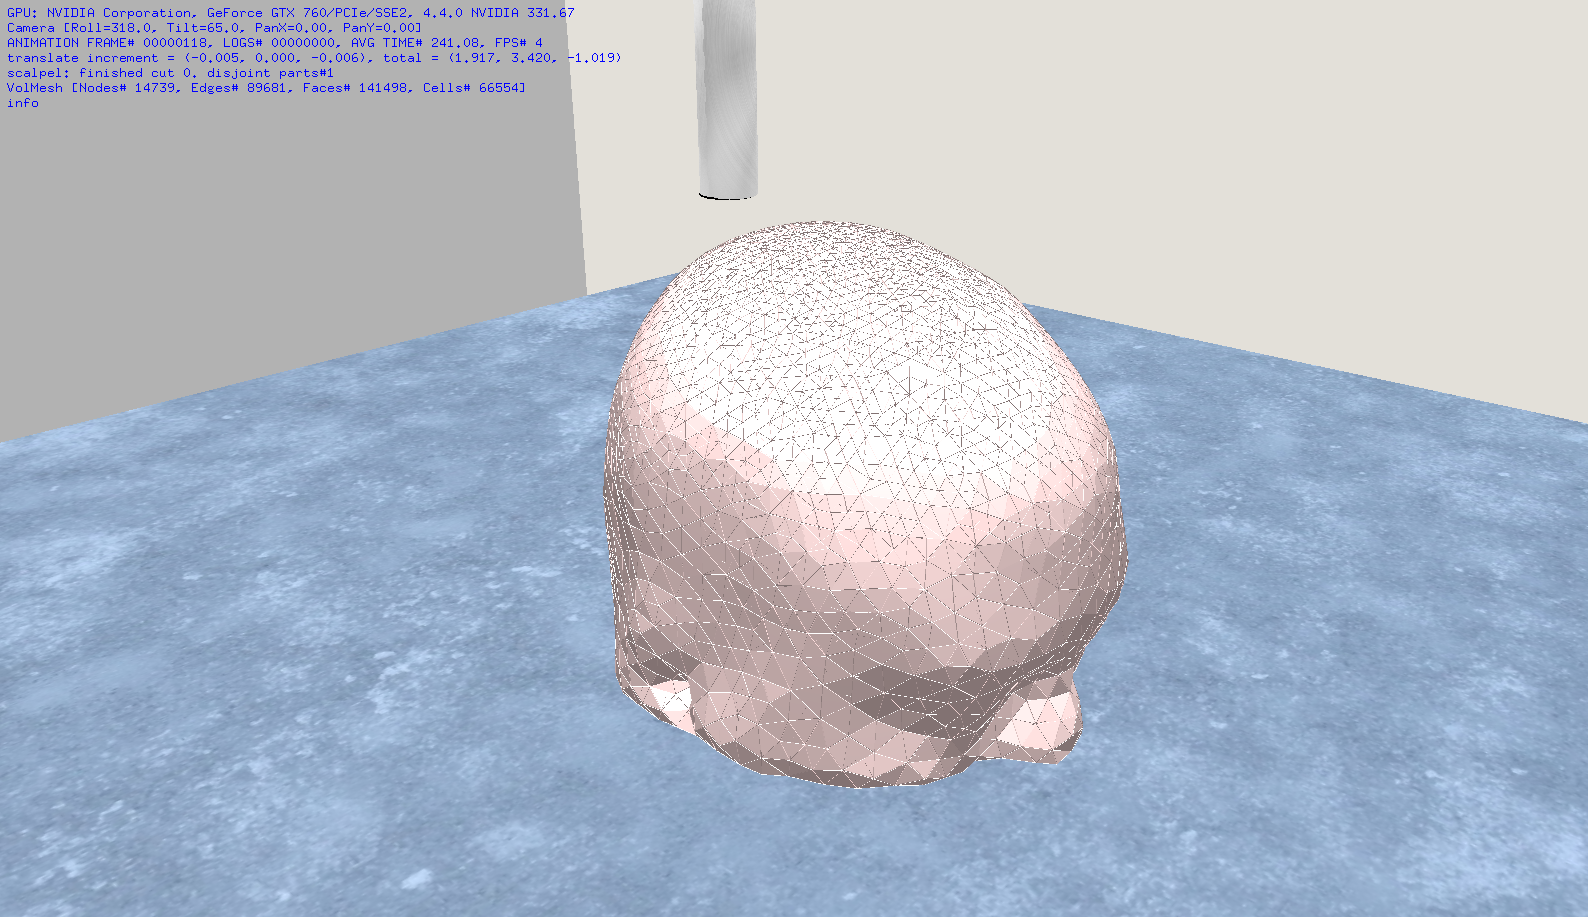
\includegraphics[width=0.7\linewidth]{figures/evaluation/craniotomy01.png}
  \caption{\label{fig:craniotomy01}
  {The scene setup for the craniotomy operation.}
}
\end{figure}


The cutting tool in this scenario is a tube-shaped device which can drill into the skull tissue and separate the bone matter.
In our system, the tool is defined as a curve approximated by $N$ line segments. The tool movement is tracked in the space 
and the system checks for collisions between the tool and the model continuously. Figure \ref{fig:craniotomytube} shows the 
polygonal shape of the cutting tool while in contact with the skull tissue.

\begin{figure}[H]
  \centering
  % the following command controls the width of the embedded PS file
  % (relative to the width of the current column)
  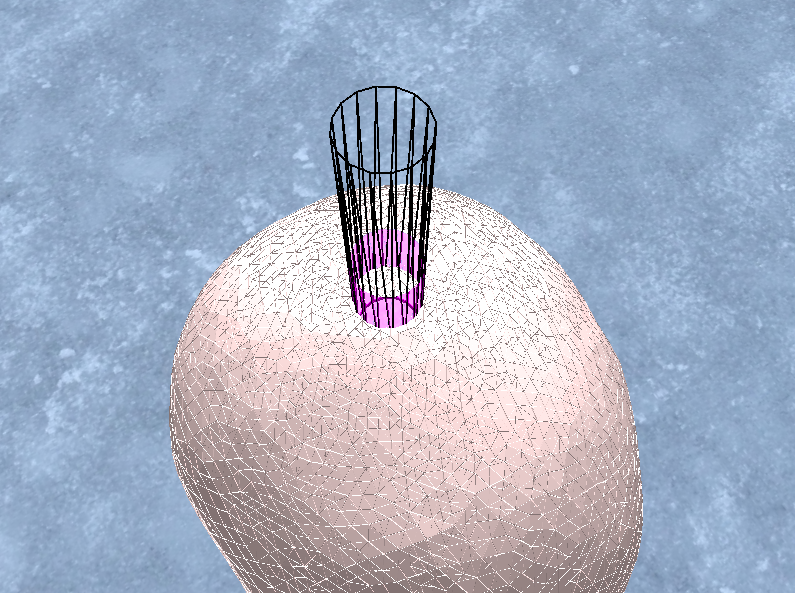
\includegraphics[width=0.6\linewidth]{figures/evaluation/craniotomytube.png}
  \caption{\label{fig:craniotomytube}
  {Cutting tool is defined as a tube with a base composed of a curve approximated with $N$ line segments. 
  Collisions between the tool and the tissue are monitored constantly.}
}
\end{figure}

When in contact with the skull tissue the intersection of the side wall of the tool is computed against the edges of the 
skull model. With $N$ line segments the cutting tool has $N$ quadrilateral faces on its side wall, the edge intersection 
test is performed in our system by calling the kernel function given in algorithm \ref{alg:edgeIntersections} once per each quad.
After each call the hash-table storing the cut-edges is filled with the new cuts. In case an edge is cut twice by the tool only 
the first cut is retained. This situation happens when a long edge of the tissue model is cut by relatively shorter segments of 
the cutting tool which is also illustrated in figure \ref{fig:ringscalpalissue}.

\begin{figure}[H]
  \centering
  % the following command controls the width of the embedded PS file
  % (relative to the width of the current column)
  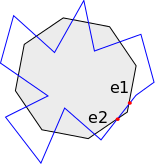
\includegraphics[width=0.2\linewidth]{figures/evaluation/ringscalpalissue.png}
  \caption{\label{fig:ringscalpalissue}
  {An edge in the volumetric mesh model is cut by multiple segments of the scalpel (Intersection points are shown in red dots)
   Only the first intersection is accepted in this case.}
}
\end{figure}


The cutting configurations presented in section \ref{sec:cutconfigs} are extracted based on one intersection per edge, therefore
it's not possible to cut a given edge more than once. In our system we only accept the first cut-edge and this did not produce any 
visual defects. Perhaps a more robust implementation would be to approximate the cutting tool curve based on the size of the longest 
edge in the mesh. After the cutting is made the mesh is separated and each of the disconnected parts is converted into a separate node
in our scene-graph structure. This operation results in correct detection of the self-collisions in the subsequent frames of the simulation.

The internal gray, white and CSF matters are also included in this simulation. The drilling operation only affects the skull tissue and
in fact it does not pass the Dura layer. This condition is a requirement for the successful completion of this procedure. 

Figure \ref{fig:crosssection} shows the cross section view of the brain. The skull is cut with a scalpel tool 
to show the internal tissues which are drawn in blue for better visibility. 
\begin{figure}[H]
  \centering
  % the following command controls the width of the embedded PS file
  % (relative to the width of the current column)
  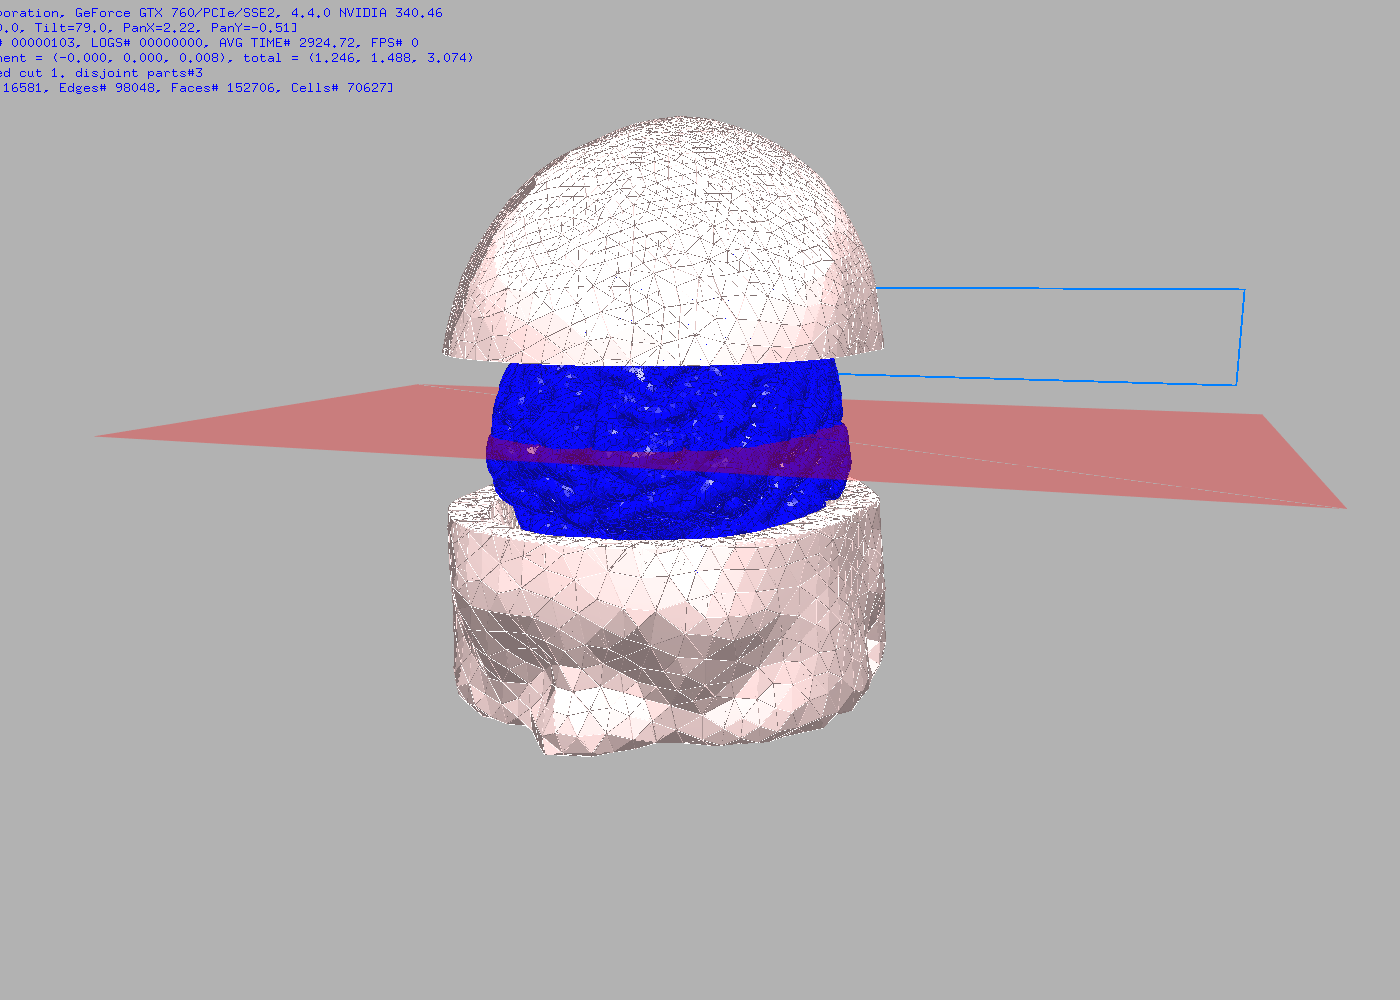
\includegraphics[width=0.5\linewidth]{figures/evaluation/crosssection.png}
  \caption{\label{fig:crosssection}
  {Cross section view of the brain layers. The skull shown in pink is cut using a scalpel avatar to show 
   all the other layers depicted in blue.}
}
\end{figure}

\begin{figure}[H]
  \centering
  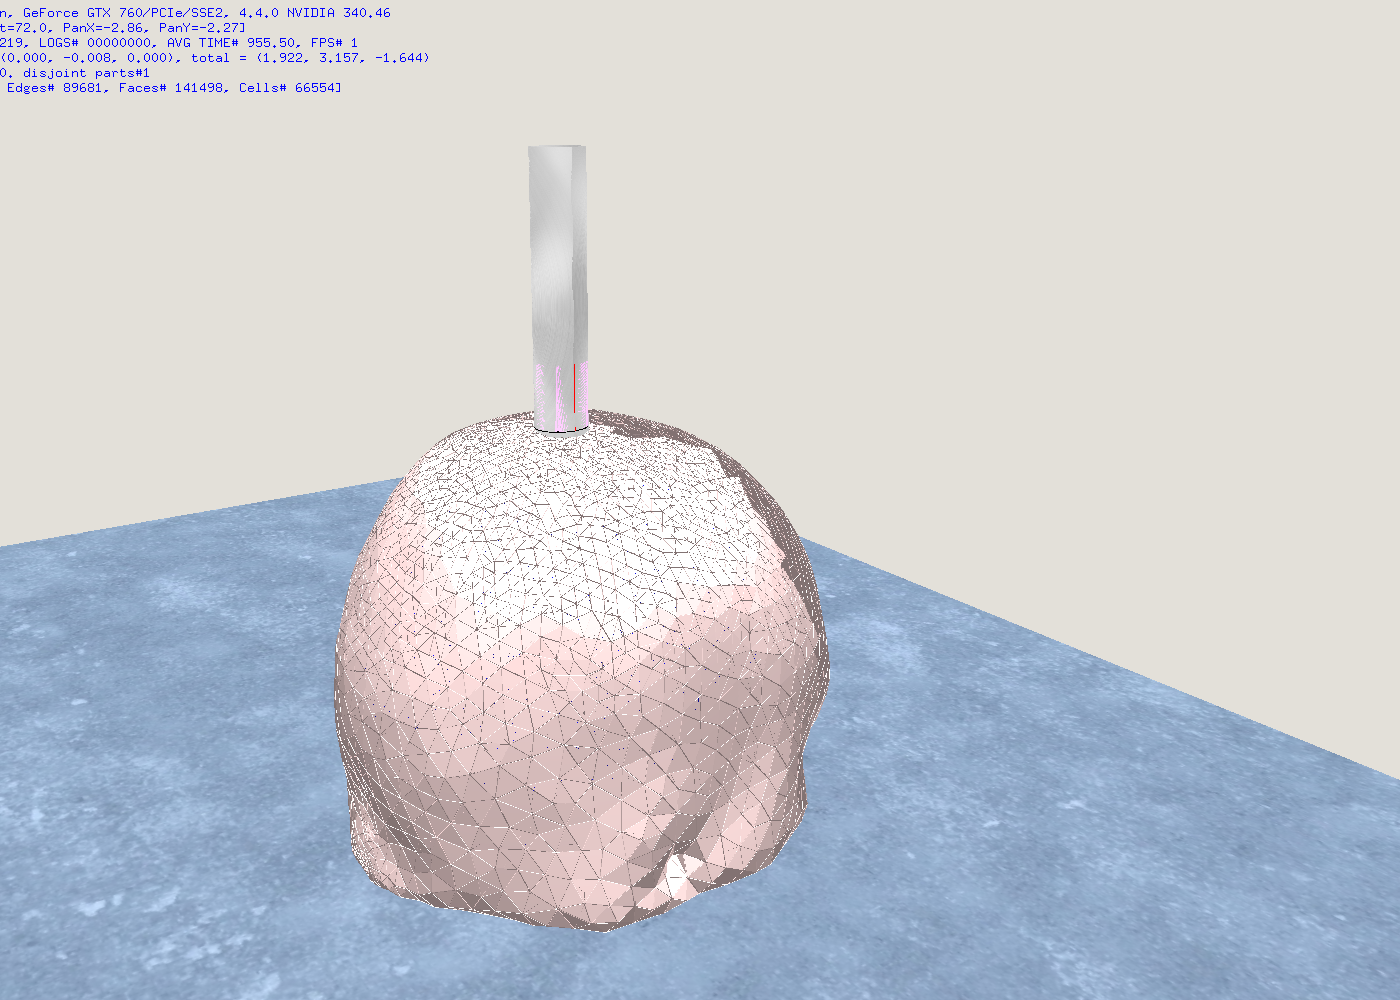
\includegraphics[width=0.5\linewidth]{figures/evaluation/craniotomy06.png}
  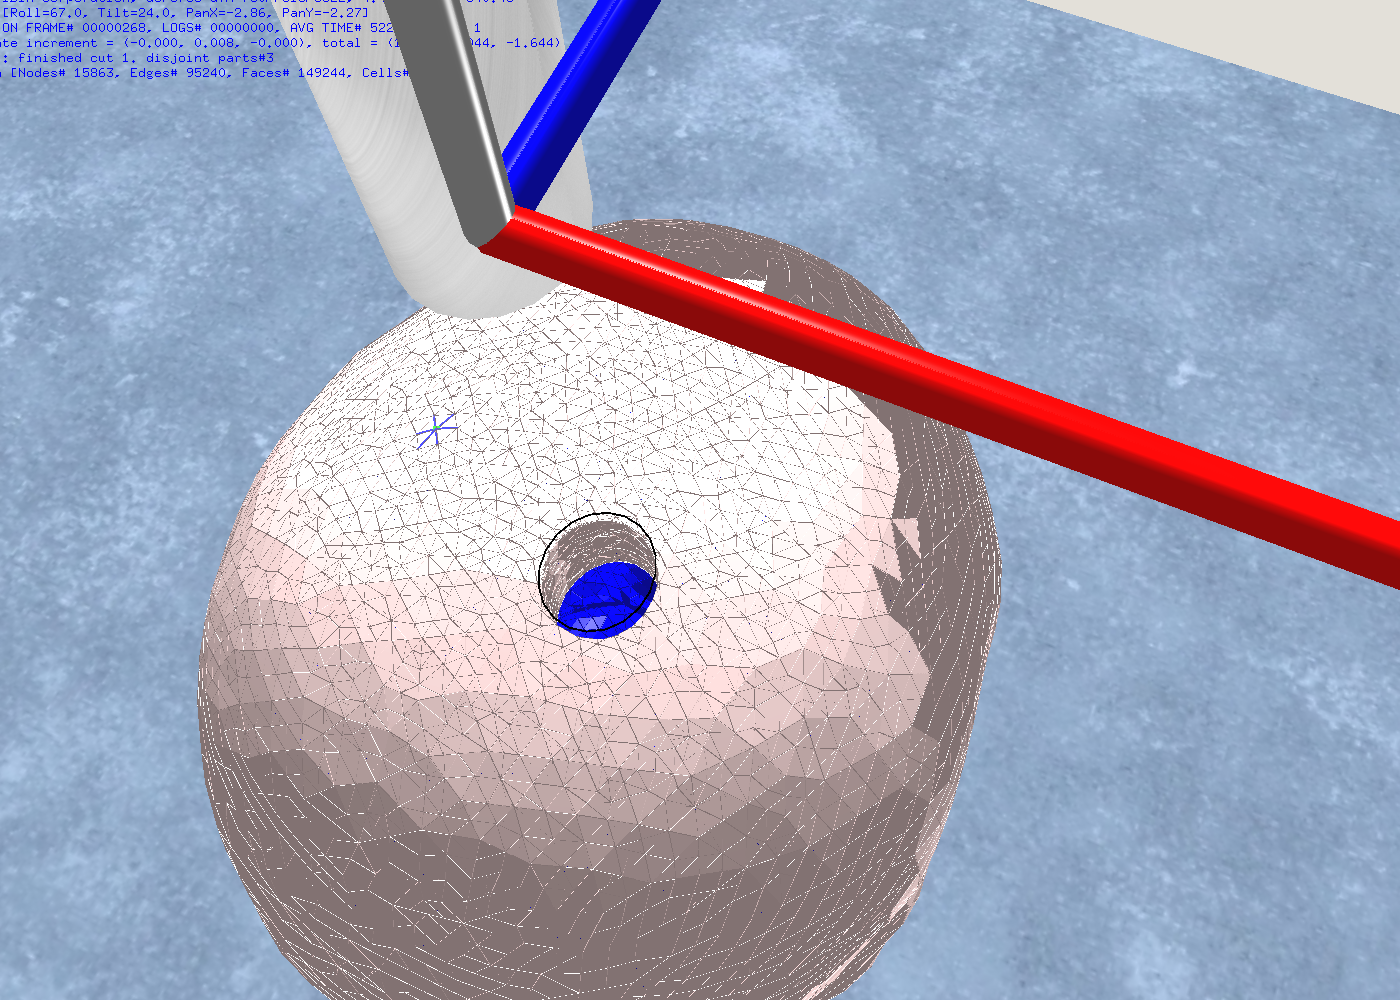
\includegraphics[width=0.5\linewidth]{figures/evaluation/craniotomy07.png}
  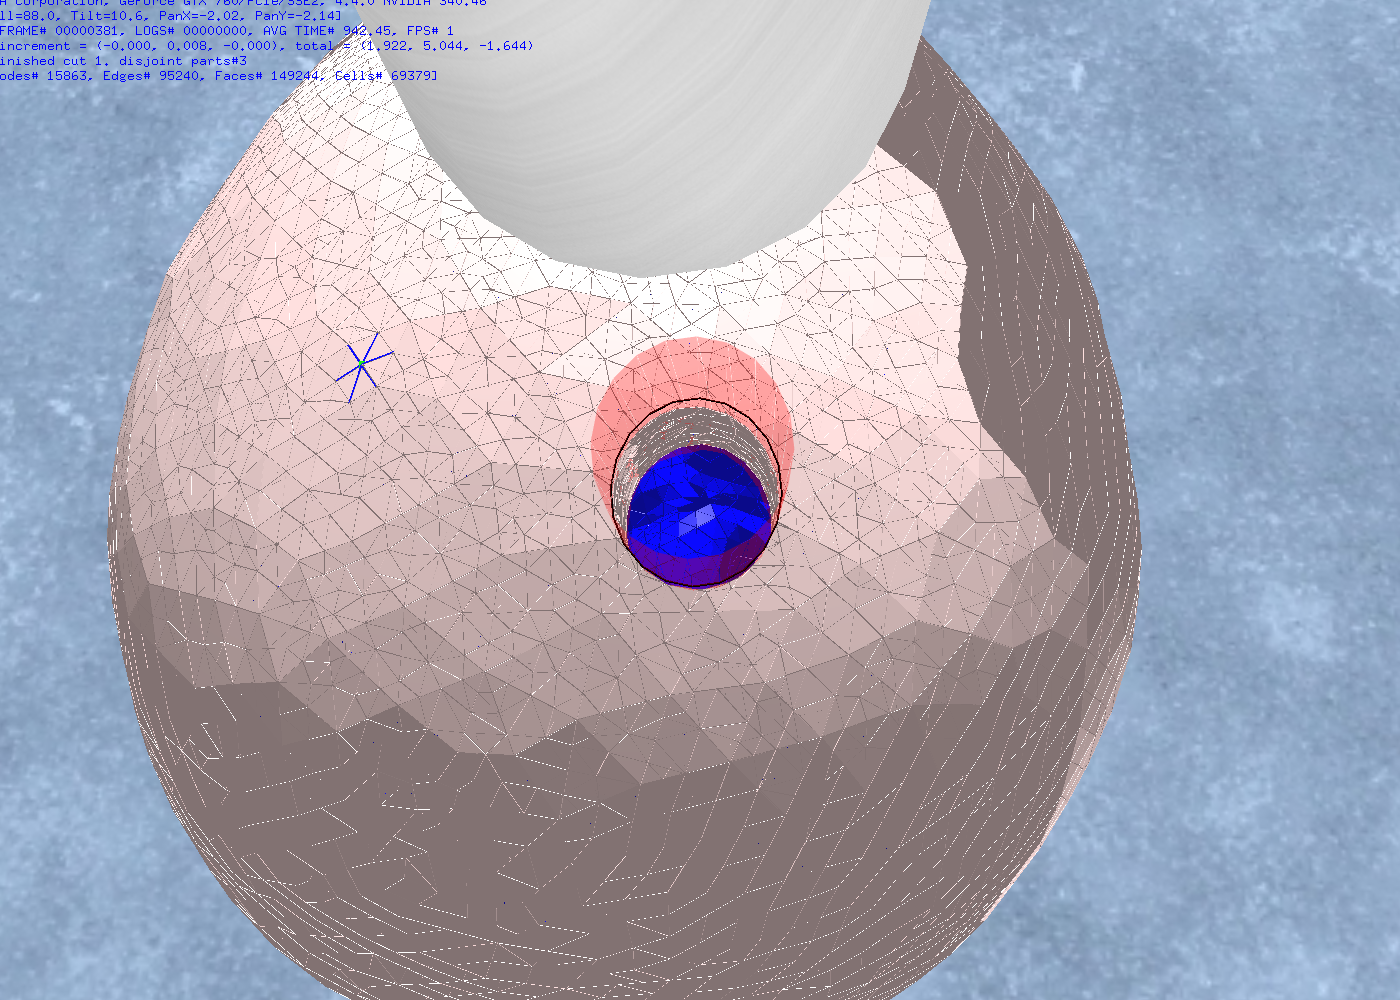
\includegraphics[width=0.5\linewidth]{figures/evaluation/craniotomy08.png}
  \caption{\label{fig:craniotomy}
  {Simulation of the craniotomy operation using our surgical simulation framework with support for interactive cutting.}
}
\end{figure}

Figure \ref{fig:craniotomy} shows the three stages of the operation (before, during and after the cutting operation). 
During the drilling process 845 tetrahedral cells are being cut in the vicinity of the drilling tool. The interaction of the drilling tool and the skull 
was interactive at all times supporting at least 60 frames per second.
        \startchapter{Conclusions}
\label{chapter:conclusion}
The following contributions were made:


\begin{enumerate}
  
\item A comprehensive modelling framework supporting a broad set of skeletal implicit primitives, 
 sketched primitive objects, warping, blending, affine transformations and constructive solid geometry 
 operators in the compact \blob structure. Our framework also provides a software architecture for 
 physically-based animation of rigid and deformable models.
 
 \item An algorithm for interactive polygonization of implicit surfaces on multi-core architectures with 
 SIMD instructions (peer reviewed). 
 
 \item An optimized GPU-accelerated algorithm for high-performance polygonization of implicit surfaces 
 on many-core architectures. 
 
 \item A novel mesh data-structure suitable for storing dynamic meshes on the GPU to support realtime 
 modifications during cutting
 
 \item Smooth, interactive cutting for complex elastic and rigid tissues 
 
% \item A novel technique for collision detection using implicit fields which is used in our system to detect 
%the intersection of the scalpel tool with the volume mesh in real-time. 
 
\item A real-time Craniotomy simulation for neurosurgery and biopsy simulations.

\end{enumerate} 

% 1. modelling framework
Our modelling framework enables physically-based animation of deformable models. 
This is better than what has been done by Cani \etal \cite{Grascuel1997}.  

% 2. SIMD polygonization method
Our SIMD polygonization method is peer reviewed \cite{Shirazian2012}. 
The proposed algorithm is scalable, dynamic and data-driven as opposed to the related work in this 
area where the input model can be either simple static functions or constant range data-sets 
\cite{Johansson2006, Tatarchuk2007, Knoll2007, Yang2010}.

% 3. GPU accelerated polygonization
Our proposed SIMD polygonization method is later optimized for using GPU acceleration. The 
proposed compact data-structure for \blob in section \ref{sec:datastructure} enables the transfer and 
rendering of large \blob in the order of 60,000 nodes interactively (as shown in that chapter using our 
compact data-structure a 64K nodes \blob only takes about 20 MB in video memory).  The result is a 
high performance polygonization method that enabled real-time updates in our incremental modelling 
system. This result is better than the work of \cite{Knoll2007, Yang2010, singh2010real, chochlik2012gpu}.
 
% 4. GPU based dynamic mesh
An intuitive volumetric mesh data-structure is proposed which is suitable for storing dynamic meshes on 
the GPU to support realtime modifications during cutting. Our cutting results show that the presented 
data-structure is more performant and can benefit the related work in this domain 
\cite{Wu2004a, Wu2005, Courtecuisse2010}.

% 5. cutting contribution how does it compare to previous work
Our proposed GPU-based data-structure enables real-time updates of the volumetric meshes upon 
cutting. Our cutting algorithm as shown in section \ref{sec:cutalg} is interactive for approximately 100,000 finite 
element cells. This is sufficient for highly complex brain surgery simulations. The resulting finite element 
cells are of high quality (the tetrahedral cells are not flat or wedge-shaped) as shown in section \ref{sec:cutres}. 
This is better than what has been done in the work of Courtecuisse \etal \cite{Courtecuisse2010}.
The cut edges are smooth, not jagged and a minimal amount of tetrahedral elements are 
created as the result of elements subdivision and this is better than the results published by Courtecuisse
\etal and Steinemann \etal \cite{Courtecuisse2010, Steinemann}. 


% 7. Craniotomy simulation
We presented a Craniotomy simulation based on our real-time cutting algorithm and the segmented 
brain data-set published by Fang \etal \cite{fang2010mesh}. 
%Although at this point we don't support haptic feedback but the simulation is well-received by one neurosurgeon at Stanford school of 
%medicine and Dr. Sandrine deRibaupierre from Western University. 
Given the large number of finite element cells in the brain mesh (around 100,000), our 
simulation still runs at interactive rates and the cutting output is smooth for a high-quality simulation 
as shown in section \ref{sec:craniotomy}. Colchester \etal used superimposed surface mesh for 
guiding a Craniotomy simulation \cite{Colchester1994}. Abe \etal used plastic skull models for 
training this procedure \cite{Abe1998}. To the best of our knowledge our proposed method is the only 
physically-based simulation for this specific procedure. 




\section{Future Work}
There are many areas in which the proposed system may be improved. The polygonization method 
introduced in chapter \ref{chapter:GPUDiscretization} can be further extended to support for more 
complex implicit primitives such as skeletal curve primitives. Such primitives can be helpful in modelling 
vain and other tube-shaped tissues. Support for implicit decals as suggested in \cite{Schmidtb} can help 
in creating realistically textured organs. 

Our cutting algorithm can also be extended to support progressive cuts. Progressive cuts can drastically 
enhance the perceived sense cutting. Also incorporating a fluid simulation will enhance the cutting 
scenario for simulating blood and CSF fluids in the brain. Procedural models such as L-Systems can be 
used to simulate the small blood vessels in the brain biopsy simulation. 

As computational power continues to increase, and optimization algorithms continue to improve, implicit 
surfaces are likely to play a much larger role in computer graphics. It is the sincere hope of the author 
that this research demonstrates what that role might be, and will encourage others to explore this domain.




	\appendix
	\startappendix{Additional Information}
\label{chapter:appendix}

This is a good place to put tables, lots of results, perhaps all the data compiled in the experiments. By avoiding putting all the results inside the chapters themselves, the whole thing may become much more readable and the various tables can be linked to appropriately.

The main purpose of an Appendix however should be to take care of the future readers and researchers. This implies listing all the housekeeping facts needed to continue the research. For example: where is the raw data stored? where is the software used? which version of which operating system or library or experimental equipment was used and where can it be accessed again?

Ask yourself: if you were given this thesis to read with the goal that you will be expanding the research presented here, what would you like to have as housekeeping information and what do you need? Be kind to the future graduate students and to your supervisor who will be the one stuck in the middle trying to find where all the stuff was left!



% The style of bibliography exemplified here is the "plain",
% normally used in science theses. This is shown
% by the entry {plain} below. Substitute the
% appropriate bibliography style. See also the
% PDF file "InformationOnBibliographyStyles" in this
% directory for more choices.

% The Bibliography file is a BibTex file named
% UVicThesis.bib and called below

	\TOCadd{Bibliography}
	\bibliographystyle{plain}
	\bibliography{PouryaLibrary}

\end{document}
